
\documentclass[]{report}\usepackage[]{graphicx}\usepackage[]{color}
%% maxwidth is the original width if it is less than linewidth
%% otherwise use linewidth (to make sure the graphics do not exceed the margin)
\makeatletter
\def\maxwidth{ %
  \ifdim\Gin@nat@width>\linewidth
    \linewidth
  \else
    \Gin@nat@width
  \fi
}
\makeatother

\definecolor{fgcolor}{rgb}{0.345, 0.345, 0.345}
\newcommand{\hlnum}[1]{\textcolor[rgb]{0.686,0.059,0.569}{#1}}%
\newcommand{\hlstr}[1]{\textcolor[rgb]{0.192,0.494,0.8}{#1}}%
\newcommand{\hlcom}[1]{\textcolor[rgb]{0.678,0.584,0.686}{\textit{#1}}}%
\newcommand{\hlopt}[1]{\textcolor[rgb]{0,0,0}{#1}}%
\newcommand{\hlstd}[1]{\textcolor[rgb]{0.345,0.345,0.345}{#1}}%
\newcommand{\hlkwa}[1]{\textcolor[rgb]{0.161,0.373,0.58}{\textbf{#1}}}%
\newcommand{\hlkwb}[1]{\textcolor[rgb]{0.69,0.353,0.396}{#1}}%
\newcommand{\hlkwc}[1]{\textcolor[rgb]{0.333,0.667,0.333}{#1}}%
\newcommand{\hlkwd}[1]{\textcolor[rgb]{0.737,0.353,0.396}{\textbf{#1}}}%
\let\hlipl\hlkwb

\usepackage{framed}
\makeatletter
\newenvironment{kframe}{%
 \def\at@end@of@kframe{}%
 \ifinner\ifhmode%
  \def\at@end@of@kframe{\end{minipage}}%
  \begin{minipage}{\columnwidth}%
 \fi\fi%
 \def\FrameCommand##1{\hskip\@totalleftmargin \hskip-\fboxsep
 \colorbox{shadecolor}{##1}\hskip-\fboxsep
     % There is no \\@totalrightmargin, so:
     \hskip-\linewidth \hskip-\@totalleftmargin \hskip\columnwidth}%
 \MakeFramed {\advance\hsize-\width
   \@totalleftmargin\z@ \linewidth\hsize
   \@setminipage}}%
 {\par\unskip\endMakeFramed%
 \at@end@of@kframe}
\makeatother

\definecolor{shadecolor}{rgb}{.97, .97, .97}
\definecolor{messagecolor}{rgb}{0, 0, 0}
\definecolor{warningcolor}{rgb}{1, 0, 1}
\definecolor{errorcolor}{rgb}{1, 0, 0}
\newenvironment{knitrout}{}{} % an empty environment to be redefined in TeX

\usepackage{alltt}
\usepackage[english]{babel}
\usepackage{graphicx}





% Title Page
\title{Analyzing data using linear models}

\author{Stephanie van den Berg}
\date{Versie 0.1 \\ (\today)}
\IfFileExists{upquote.sty}{\usepackage{upquote}}{}
\begin{document}
\maketitle




\begin{abstract}
This book is intended to be of use to bachelor students in social sciences that want to learn how to analyze their data, with the specific aim to answer research questions. The book has a practical take on data analysis: how to do it, how to interpret the results, and how to report the results. All techniques are presented within the framework of linear models: this includes simple regression models, to linear mixed models, and generalized linear models. All methods can be carried out within one supermodel: the generalized linear mixed model. This approach is illustrated using SPSS.
\end{abstract}


\tableofcontents



\chapter{Exploring your data}

\section{Types of variables}
Data analysis is about variables. In linear models there are different kinds of variables. One important distinction is between dependent variables and independent variables. The other important distinction is about the measurement level of the variable: continuous, ordinal or categorical. 


\subsection{Continuous, ordinal, and categorical variables}
A typical example of a contiuous variable is age: in theory, you could calcualate your age in the number of minutes that have passed since your time of birth. It is continuous in the sense that it has an (almost) infinite number of possible values. For example, for two children born one minute a part, there could be a third child that was born just in between the other two. In practice of course, we measure age in days, and sometimes only in months in years, but given there are many values, we usually treat such an age variable in years as continuous. Other examples of continuous variables include height in inches, temperature in degrees Celcius, years of education, or systolic bloodpressure in millimeters of mercury. Note that in all these examples, quantities (age, height, temperature) are expressed as the number of a particlar unit (years, inches, degrees). Therefore continuous variables are often called quantitative variable, or quantitative measures. There is a further distinction into interval and ratio variables; this distinction is treated in the research methods course in Module 1.

With ordinal measures, there are no units. An example would be a variable that would quantify size, by stating whether a t-shirt is small, medium or large. Yes, there is a quantity here, size, but there is no unit to state EXACTLY how much of that quantity is available. Similar for age, we could code a number of people as young, middle-aged or old, but on the basis of such a variable we could not state by \textit{how much} two individuals differ in age. Ordinal data are usually \textit{discrete}: there are no infinite number of levels of the variable. It goes up in discrete steps, for example, having values of 1, 2 and 3, and nothing in between.

Lastly, categorical variables are not about quantity at all. Categorical variables are about quality. A typical example of a categorical variable would be the colour of pencils: they can be either green, blue, black, white, red, yellow, etcetera. Nothing quantitative could be stated about a bunch of pencils that are only assessed regarding their colour, other than saying that a green pens are greener than other pens, and red pens are redder than other pens. There is usually no logical order in the values of such variables. Other examples include nationality (French, Turkish, Indian, other) or sex (male, female, other). Categorical variables are often called nominal variables, or qualitative variables.

\subsubsection{Exercises} 
In the following, identify the type of variable in termes of continuous, ordinal discrete, or categorical:\\
Age: \dots years\\
Weight: \dots kilograms\\
Size: \dots meters\\
Size: small, medium, large\\
Exercise intensity: low, moderate, high\\
Agreement: not agree, somewhat agree, agree\\
Agreement: totally not agree, somewhat not agree, neither disagree nor agree, somewhat agree, totally agree\\
Pain: 1, 2.. ..... , 99, 100\\
Quality of life: 1=extremely low, \dots, \dots, 7=extremely high\\
Colour: blue, green, yellow, other\\
Nationality: Chinese, Korean, Australian, Dutch, other\\
Gender: Female, Male, other \\
Gender: Female, Male
Number of shoes: \\




\subsection{Qualitative and quantitative treatment of variables in data analysis}
There is a fundamental difference between continuous and ordinal variables, but it is possible to treat them the same way in data analysis. For data analysis with linear models, you have to decide for each variable whether you want to treat it as qualitative or quantitative. Continuous variables are always treated as quantitative. Categorical data are always treated as qualitative. The problem is with ordinal variables: you can either treat them as quantitative variables or as qualitative variables. The choice is usually based on common sense and whether the results are meaningful. For instance, if you have an ordinal variable with 8 levels, like a Likert scale, it usually does not make sense to treat it as qualitative. If the variable has only 3 levels, it is often meaningful to treat it as qualitative: assuming that the three levels can show qualitative differences. In the coming chapters, we will come back to this distinction. Remember, in the coming chapters we will only speak of quantitative and qualitative treatment of variables, and remember that continuous variables are always treated as quantitative and categorical data are always treated as qualitative.


\subsection{Dependent and independent variables}
So now that we have discussed the distinction between continuous, ordinal and categorical variables, let's turn to dependent and independent variables. Determining whether a variable is treated as independent or not, is often either a case of logic or a case of theory. When studying the relationship between the height of a father and that if his child, the more logical it would be to see the height of the child **as a function** of the height of the father. This because we assume that the genes are transferred from the father to the child. The father comes first, and the height of the child is partly the *result* of the genes that were transmitted during fertilisation. Similarly, when predicting precipitation on the basis of the hours of sun light on the previous day, it seems natural to study the effect of hours of sunlight on the previous day on precipitation on the next day. That which is the result is usually taken as the dependent variable. The theoretical cause or antecedent is usually taken as the independent variable. \\
The dependent variable is often called the \textit{response variable}. An independent variable is often called a \textit{predictor variable} or simply \textit{predictor}.

Examples: the effect of income on health

size is caused by inflation

size is influenced by weight

shoe size is predicted by sex


\subsubsection{Exercises} 


From each of the following statements, identify the dependent variable and the independent variable:

The less you drink the more thirsty you become \\
The more calories you eat, the more you weigh\\
Weight is affected by food intake \\
Weight is affected by exercise \\
Food intake is predicted by time of year \\
There is an effect of exercise on heart rate \\
Inflation leads to higher wages \\
Unprotected sex leads to pregnancy \\
HIV-infection is caused by unprotected sex\\
The effect of alcohol intake on driving performance\\
Sunshine causes growth
 % exploring your data


\chapter{Linear modelling: introduction FULYA}
\section{Linear relationships}
\section{Pearson correlation}
\section{Simple regression with a continuous predictor}
\section{Predicting the dependent variable}


\chapter{Multivariate regression}
\section{R-squared}

\chapter{Inference MARIAN}
\section{Random sampling and confidence intervals}
\section{$t$-statistics, null-hypothesis testing and $p$-values}
\section{Inference: from sample to population}




\chapter{Categorical predictor variables}
\section{Dummy coding}
\section{Predicting group means}
\section{Dummy coding for more than two groups}
\section{Comparing more than two groups}


In previous sections we used dummy coding for categorical variables with two levels. Now we look into the situation where you have a categorical variable that has more than 2 levels. Take for instance the variable Country, where in your data set, there are three different values for this variable, for instance, Norway, Sweden and Finland, or perhaps Zimbabwe, Congo and South-Africa. Let's call these countries A, B and C. Here's a data example:
 \\
 \\
 \begin{tabular}{llr}
 ID & Country &  height\\ \hline
  001 &A & 120\\
  002 &A & 160\\
  003 &B & 121\\
  004 &B & 125\\
  005 &C & 140\\
  \dots & \dots & \dots\\
 \end{tabular}
\\
\\
In general, when we have 3 different values for a categorical variable, we can code this into two dummy variables in the following way.




Let's take country C as our reference category: that means we want to know whether observations from countries A and B differ from observations from country C. So we code one new dummy variable with 1s for country A and 0s for the other countries. We code a second new dummy variable with 1s for country B and 0s for the other countries. So we get the new data file:
 \\
 \\
 \begin{tabular}{llrrr}
 ID & Country &  height & CountryA & CountryB \\ \hline
  001 &A & 120 & 1 & 0\\
  002 &A & 160 & 1 & 0\\
  003 &B & 121 & 0 & 1\\
  004 &B & 125 & 0 & 1\\
  005 &C & 140 & 0 & 0\\
  \dots & \dots & \dots& \dots & \dots\\
 \end{tabular}
\\
\\
Note that a third dummy variable CountryC is not necessary. Remember that with two categories, you only need one dummy variable, where one level gets 1s and another category gets 0s. In this way both categories are uniquely identified. Here with three categories we also have unique codes for every category: 1 and 0 for country A, 0 and 1 for country B, and 0 and 0 for country C. Similarly, if you have 4 categories, you can code this with 3 dummy variables. In general, when you have a variable with $K$ categories, you can code them with $K-1$ dummy variables.







\subsection{Analyzing categorical predictor variables}

Suppose we have data on height based on a sample of thirty people ($N=30$) that come from three different countries. We want to know whether the average height is different for each country, or whether the average height is the same (null-hypothesis). We want to analyze this with a linear model in SPSS. Now there are two ways of doing this. First option is that you can use dummy coding first, and then treat these dummy variables in a quantitative way. The second option is that you let SPSS do the dummy coding for you, by indicating that you want to treat the original variable as qualitative. Let's start with the first option and then discuss the second option. Afterwards we will compare these two options.

\subsubsection{Treating dummy variables quantitatively}


First we create two new dummy variables, and then perform a linear model analysis using these. Note that we actually perform a multiple regression with two dummy variables.


\begin{verbatim}
RECODE Country ('A'=1) ('B'=0) ('C'=0) INTO CountryA.
RECODE Country ('A'=0) ('B'=1) ('C'=0) INTO CountryB.
EXECUTE.
UNIANOVA height WITH CountryA CountryB 
/ design = CountryA CountryB
/ print = parameter.
\end{verbatim}


\begin{figure}[h]
    \begin{center}
       \includegraphics[scale=0.5]{/Users/stephanievandenberg/Dropbox/Statistiek_Onderwijs/Data" "Analysis/spss" "examples" "mixed" "linear" "model/oneway/onewayquant.png}
    \end{center}
\end{figure}


In the Parameter Estimates table, we see the effects of the two dummy variables. All observations with a 1 for variable CountryA get an extra predicted height of -2.4, and all observations with a 1 for variable CountryB get an extra predicted height of 10.1. So the expected height in country A equals $172.4 - 2.4 = 174.8$, and the expected height in country B equals $172.4+10.1=182.5 $. Observations in country C have a 0 for both variables CountryA and CountryB, so the expected height in country C equals the intercept 172.4.\\

In the Tests of between-subjects Effects table, we see other stuff going on. This is not regression output, but output based on a so-called Analysis Of VAriance, or ANOVA for short. First note that the significance levels for the two effects are exactly the same as those from the regression table. Second, note that the reported values of $F$ are the square of the $t$ values in the regression table: $-.799^2=.619$ and $3.364^2=11.317$. \\
ANOVA is a particular case of a linear model. The $F$-statistic is constructed on the basis of Sums of Squares. For instance, take a look at the row for the effect of CountryA. The sum of squares is equal to 28.80. If you divide this by the degrees of freedom for this effect, your get the Mean Square: $28.80/1=28.80$. Now look at the row for Error. The sum of squares equals 1216.90. Divided by the corresponding degrees of freedom you get the Mean Square: $12.16.90/27=45.07$. You obtain the $F$-statistic by dividing the CountryA Mean Square by the Error Mean Square: $F=28.80/45.07=0.639$. 
It is not a coincidence that this $F$-value is exactly equal to the square of the corresponding $t$-value: $F=t^2$. Remember that the $t$-value is equal to the $B$ parameter divided by the standard error: $t=-2.400/3.002=-.799=\sqrt{0.639}$. To obtain the regression coefficient we minimize the sums of squares of the residuals. So both the $F$-statistic and the $t$-statistic come from computing sums of squares and are thus based on the same general logic of the linear model.\\

Since ANOVA is a special case of the linear model, we believe that it is not necessary to understand ANOVA fully: if you understand the linear model, that is good enough. Just remember that sometimes you see ANOVAs reported in the literature. Be aware that what they are actually doing is running a linear model.




\subsubsection{Treating the original variable qualitatively}

In the alternative approach, we let SPSS do the dummy variable coding automatically. In that case we use the original variable Country with its three categories directly, and change the WITH into BY in the following way:

\begin{verbatim}
UNIANOVA height BY Country 
/ design = Country
/ print = parameter.
\end{verbatim}

All variables named after BY are treated as categorical variables and automatically coded into dummy variables. The output then looks like the following:

\begin{figure}[h]
    \begin{center}
       \includegraphics[scale=0.5]{/Users/stephanievandenberg/Dropbox/Statistiek_Onderwijs/Data" "Analysis/spss" "examples" "mixed" "linear" "model/oneway/onewayqual.png}
    \end{center}
\end{figure}

The Parameter Estimates table now looks slightly different: The intercept is the same, the dummy effects are presented in a slightly different way, and there is an extra row for country C where a regression coefficient $B$ of 0 is reported, with no other information. The values for the other effects are exactly the same as with the previous analysis. This means we can interpret these country=A and country=B effects as the effects of dummy variables: all observations start from an intercept of 172.40 and depending on whether the observation from country A or country B, you get an extra predicted height of -2.4 or 10.1, respectively. Observations from country C get an extra height of 0, so in effect nothing extra. (It seems that what SPSS is doing is creating an extra dummmy variable for country C, but because this is not necessary, the effect is fixed to 0).
\\
Also the Tests of Between-Subjects Effects table looks slightly different: instead of two separate effects for two dummy variables, we now see one row for the original variable Country. And in the column df (degrees of freedom), instead of 1 degree of freedom for a country effect, we see 2 degrees of freedom. So this suggests that the effects of the two dummy variables are now combined into one effect, with a particular $F$-value, and a p-value that is also different from those of the two separate dummy variable. This is actually the test for the null-hypothesis that all 3 means are equal. This is very differnt from the t-tests in the Parameter Estimates table. The $t$-test for the country=A effect specificically tests whether the average height in country A is different from the average height in counry C (the reference country). The $t$-test for the country=B effect specifically tests whether the average height in country B is different from the average height in country C (the reference country). Since these do not refer to our research question regarding overall differences across all three countries, we do not report these $t$-tests, but report the overal $F$-test from the Tests of Between-Subjects Effects table.

\subsubsection{Reporting one-way ANOVA}
In all cases where you have a categorical predictor variable with more than two categories, and where the null-hypothesis is about the equality of all means, you always report the $F$-statistic from the Tests of Between-Subjects Effects. You do that in the following way for this particular example:

\begin{quote}
``The null-hypothesis that all 3 means were equal was tested with a linear model (one-way analysis of variance). The results showed that the means in the population are not equal, $F(2, 27)=9.76, MSE=45.07 , p < 0.05$.''
\end{quote}

Always check the degrees of freedom of for your $F$-statistic. The first number refers to the number of dummy variables that are tested at once: this is the number of categories minus 1. The second number refers to the error degrees of freedom: this is the number of observations minus the number of effects in your model. In this model you have 30 data points and you have three effects (parameters): one intercept, one effect for Country=A, and one effect for Country=B. So your error degrees of freedom is $30-3=27$. Note that this error degrees of freedom is equal to that of the $t$-statistic. 



\section{$F$-test for multiple group comparisons}
 % dummy variables and categorical predictors


\chapter{Moderation: testing interaction effects}
\section{Categorical by linear interaction}



Suppose there is a linear relationship between age and vocabulary: the older you get, the more words you know. Suppose we have the following linear regression equation for this relationship:


\begin{eqnarray}
vocab = 200 + 500 \times age + e
\end{eqnarray}

So according to this model, the expected number of words for a newborn baby (age=0) equals 200. This may sound silly, but suppose this model is a very good model for vocabulary size in children between 2 and 5 years of age. Then this equation tells us that the expected increase in vocabulary size is 500 words per year.

Now this model is meant for everybody in the Netherlands. But suppose that one researcher expects that the increase in words is much faster in children from high SES families than in children from low SES families. First he believes that vocabulary will be larger in higher SES children than in low SES children. In other words, he expects an effect of SES, over and above the effect of age:

\begin{eqnarray}
vocab = 200 + 500 \times age + \beta_2 \times SES + e
\end{eqnarray}

This main effect of SES is yet unknown and denoted by $\beta_2$.

But he also expects that the yearly increase is a bit lower than 500 words in low SES families, and a little bit higher than 500 words in high SES families. In other words, he believes that SES might \textit{moderate} (changes) the slope coefficient. Let's call the slope coefficent in this case $\beta_1$. In the above equation it is equal to 500, but let's now let it be a linear function of SES:

\begin{eqnarray}
\beta_1 = \alpha^* + \beta_3 \times SES 
\end{eqnarray}

So let's plug this equation into the regression equation for vocabulary:

\begin{eqnarray}
vocab = 200 + \beta_1 \times age + \beta_2 \times SES + e \\
vocab = 200 + (\alpha^* + \beta_3 \times SES)  \times age + \beta_2 \times SES + e
\end{eqnarray}




Multiplying this out gets us:


\begin{eqnarray} 
vocab = 200 + \alpha^* \times age + \beta_3 \times SES  \times age + \beta_2 \times SES + e
\end{eqnarray}

If we rearrange the terms a bit, we get:


\begin{eqnarray} 
vocab = 200 + \alpha^* \times age + \beta_2 \times SES + \beta_3 \times SES  \times age + e
\end{eqnarray}

Now this very much looks like a regression equation with one intercept and three slope coefficients, we might for instance change the label $\alpha^*$ into $\beta_1$ to get a more familiar looking form:

\begin{eqnarray} 
vocab = 200 + \beta_1\times age + \beta_2 \times SES + \beta_3 \times SES  \times age + e
\end{eqnarray}

So the first slope coefficient is the increase in vocabulary for every year that age increases ($\beta_1$), the second slope coefficient is the increase in vocabulary for an increase of 1 on the SES variable ($\beta_2$), and the third slope coefficient is the increase in vocabulary for every increase of 1 on the \textit{product} of age and SES.
\\
So what does this mean exactly?
\\
Let's use some numerical example. Suppose age is coded in years, and SES is dummy coded, with a 1 for high SES and a 0 for low SES.

If we look at this equation:

\begin{eqnarray}
\beta_1 = \alpha^* + \beta_3 \times SES 
\end{eqnarray}

we see that a high positive value of $\beta_3$ increases the size of $\beta_1$, which is the effect of age on vocabulary.

Suppose we find the following solution for the regression equation:

\begin{eqnarray} 
vocab = 200 + \beta_1 \times age + \beta_2 \times SES + \beta_3 \times SES  \times age + e \\
vocab = 200 + 450 \times age + 125 \times SES + 100 \times SES  \times age + e
\end{eqnarray}

If we code low SES children as SES=0, and high SES children as SES=1, we can write the above equation into two regression equations, one for low SES children (SES=0) and one for high SES chilrden (SES=1):

\begin{eqnarray} 
vocab =  200 + 450 \times age  + e \\
vocab = 200 + 450 \times age + 125  + 100   \times age + e
\end{eqnarray}

So for low SES children, the intercept is 200 and the regression slope with age is 450, so they learn 450 words per year. For high SES children, we see the same intercept of 200, with an extra 125 (this is the main effect of SES). So effectively their intercept is now 325. For the regression slope, we now have $450 \times age+ 100   \times age$ which is of course equal to $550 \times age$. So we see that the high SES group has both a different intercept, and a different slope: the increase in vocabulary is 550 per year: somewhat steeper than in low SES children. So yes, the researcher was right: vocabulary increase per year is faster in high SES children than in low SES children. 

These two different regression lines are depicted below. It can be clearly seen that the lines have two different intercepts and two different slopes. That they have two different slopes can be seen from the fact that the lines are not parallel. One has a slope of 450 words per year and the other has a slope of 550 words per year. This difference in slope of 100 is exactly the size of the slope coefficient pertaining to the product $SES \times age$. 

\begin{knitrout}
\definecolor{shadecolor}{rgb}{0.969, 0.969, 0.969}\color{fgcolor}
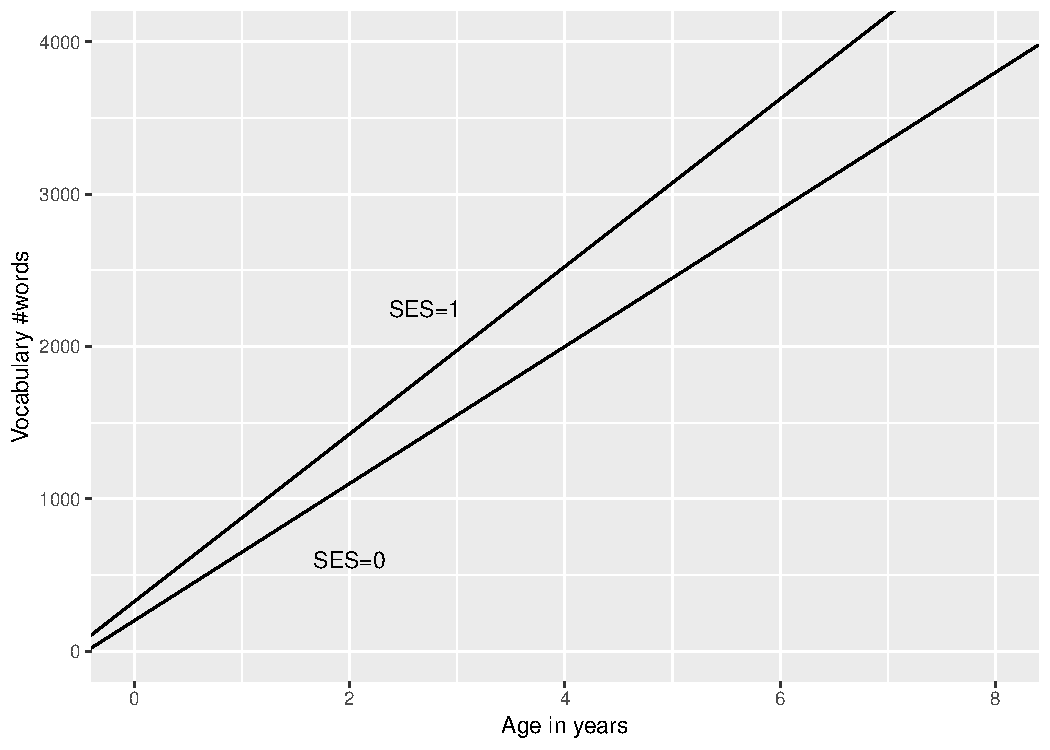
\includegraphics[width=\maxwidth]{figure/summary_plot-1} 

\end{knitrout}


The observation that the slope coefficient is different for different groups is called an \textit{interaction effect}, or \textit{interaction} for short. Other words for this phenomenon are \textit{modification} and \textit{moderation}. In this case, SES is called the \textit{modifier variable}: it modifies the relationship between age on vocabulary. (Note however that you could also interpret age as the modifier variable: the effect of SES is larger for older children than for younger children. In the plot you see that the difference between vocab for high and low SES children of age 6 is larger than it is for children of age 2.)

So, what do you have to do if you want to know if there is an interaction effect between age and SES on vocabulary size? 

First you dummy code the nominal variable SES: 


\begin{verbatim}
RECODE SES ('low'=0) ('high'=1) INTO SES_dummy.
EXECUTE.
\end{verbatim}

Next we compute a new variable, that is, the product $SES \times age$ (but use the dummy variable):


\begin{verbatim}
COMPUTE SESage = SES_dummy * age .
EXECUTE.
\end{verbatim}

So now you have three variables for a multiple regression:

\begin{verbatim}
UNIANOVA vocab WITH age SES_dummy SESage
/ design=age SES_dummy SESage.
\end{verbatim}


Note there is also a faster way of analyzing interaction effects in SPSS. The following syntax is exactly equivalent, but does not require the computation of the interaction variable $SESage$:

\begin{verbatim}
UNIANOVA vocab WITH age SES_dummy 
/ design = age SES_dummy age*SESdummy
/ print = parameter.
\end{verbatim}

With this design specification, SPSS computes the interaction variable automatically for you.
\\
Let's look at some example output for another data set. A researcher is interested in childrens' height. She has data on children between the ages of 4 and 8, with measures on their height. She wants to know whether children growing up in the city grow just as fast as in the countryside. So the data might look something like this.
 \\
 \\
 \\
 \\
 \begin{tabular}{llrr}
 child & location & age & height\\ \hline
 001 & city & 5 & 120\\
 002 & country & 14 & 160\\
 003 & city & 4 & 121\\
 004 & city & 6 & 125\\
 005 & country & 9 & 140\\
 \dots & \dots & \dots & \dots\\
 \end{tabular}
\\
\\
\\
 \\
The general regression of height on age might something like this:
\begin{knitrout}
\definecolor{shadecolor}{rgb}{0.969, 0.969, 0.969}\color{fgcolor}

{\centering 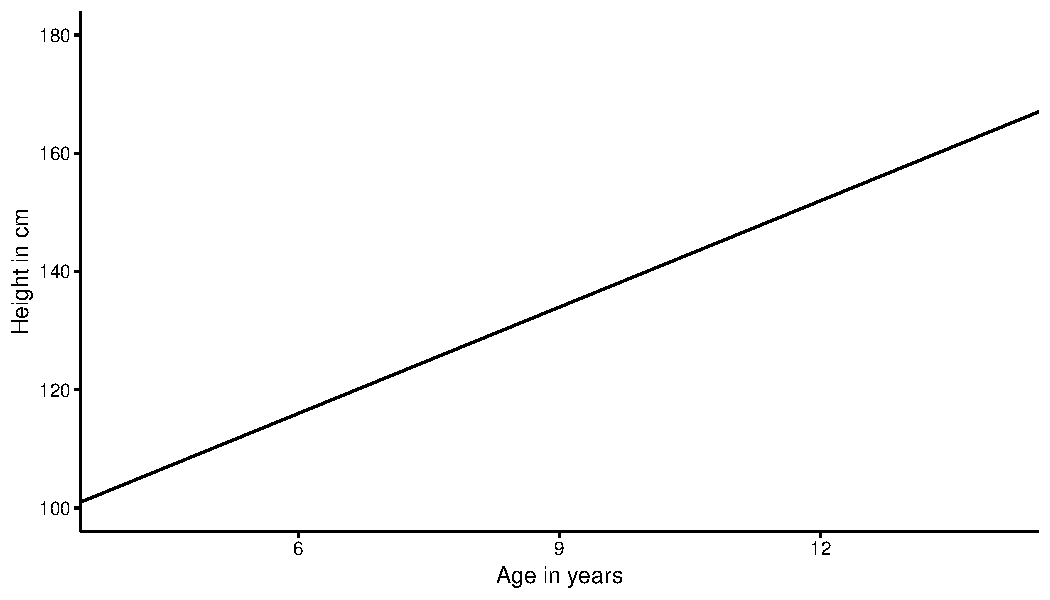
\includegraphics[width=\maxwidth]{figure/summary_plot1-1} 

}



\end{knitrout}

This regression line for the entire sample of children has a slope of around 6 cm per year. Now the researcher wants to know whether this slope is the same for children in the cities and in the countryside, in other words, do children grow as fast in the city as in the countryside? We might expect that location (city vs countryside) \textit{moderates} the effect of age on height. We use the following SPSS syntax to study this $location \times age$ effect, first creating a dummy variable for location, arbitrarily coding $country$ as 1:
\begin{verbatim}
RECODE location ('city'=0) ('country'=1) INTO location_dummy.
EXECUTE.
UNIANOVA height WITH age location_dummy 
/ design = age location_dummy  age*location_dummy
/ print = parameter.
\end{verbatim}
Below we find the corresponding SPSS output. So the null-hypothesis is that the two slopes are equal, in other words, that the interaction effect equals zero. In the output, this is the age * location\_dummy effect.


\begin{figure}[h]
    \begin{center}
       \includegraphics[scale=0.5]{/Users/stephanievandenberg/Dropbox/Statistiek_Onderwijs/Data" "Analysis/spss" "examples" "mixed" "linear" "model/interaction/interactionheight.png}
    \end{center}
\end{figure}




In the table with the parameter estimates, we find the regression coefficients. 

So we can fill in the regression equation:

\begin{eqnarray} 
height = 96 + 4.6 \times age + 3.8  \times locationdummy - 0.368 \times  age \times locationdummy + e \nonumber
\end{eqnarray}


If we fill in 0s for the location dummy, we get the equation for city children:

\begin{eqnarray} 
height &=& 96 + 4.6  \times age  + e  \nonumber
 \end{eqnarray}

So the intercept equals 96 and the slope equals 4.6.

If we fill in 1s for the location dummy variable, we get the equation for country side children:

\begin{eqnarray} 
height &=& 96 + 4.6  \times age + 3.8   - 0.368  \times age + e \\ \nonumber
      &=& (96+ 3.8) + (4.6 - 0.368) \times age + e   \nonumber
 \end{eqnarray}

We see that that the intercept is now equal to the intercept is $96+ 3.8$, and the slope equals $4.6-0.368$. 

So, we know that the slope for countryside children is 0.368 less steep than for city children. In this sample, it seems that children in the city grow 4.626 centimeters per year (on average), but that children in the countryside grow $4.626-0.368= 4.258$ centimeters per year (on average). Is this also true in the entire population of children? No, the effect of 0.368 is not significant, $t(5)=-0.23, p>0.05$. We therefore do not reject the null-hypothesis and conclude that in the population, children in the city grow just as fast as children in the countryside.\\
\\
In this  section we discussed the situation that regression slopes might be different in two groups: the regression slope might be steeper in one group than in another group. So suppose that we had a continuous predictor $x$ for a continuous dependent variable variable $y$, we said that a particularly dummy variable $z$ moderated the effect of $x$ on $y$. This moderation was quantified by an interaction effect, $x \times z$.
\\
\\
So suppose we have the following regression equation:


\begin{eqnarray} 
y = - b_0 + b_1  \times x + b_2  \times dummy +b_3 \times x \times dummy + e \nonumber
\end{eqnarray}

Here, we call $b_0$ the intercept, $b_1$ the main effect of $x$, $b_2$ the main effect of the dummy variable, and $b_3$ the interaction effect of $x$ and the dummy. 


\subsection{Exercises}


We have the following regression equation, with $y$ as dependent variable, $x$ as a continuous predictor variable, and a dummy variable $dummy$.
\\
\begin{eqnarray} 
y = 5.3 + 3.6  \times x + 3.8  \times dummy + 8.2  \times x  \times dummy + e \nonumber
\end{eqnarray}
\\
Write down the regression equation in the case the dummy variable equals 0.\\
Write down the regression equation in the case the dummy variable equals 1.\\
What is the slope if the dummy variable equals 0?\\
What is the slope if the dummy variable equals 1?\\
How large is the difference in slopes between the two groups?\\
\\
\\
We have the following regression equation, with $y$ as dependent variable, $x$ as a continuous predictor variable, and a dummy variable $dummy$.
\\
\begin{eqnarray} 
y = - 4.1 + 1.2  \times x - 6.5  \times dummy - 1.3 \times x \times dummy + e \nonumber
\end{eqnarray}
\\
Write down the regression equation in the case the dummy variable equals 0.\\
Write down the regression equation in the case the dummy variable equals 1.\\
What is the slope if the dummy variable equals 0?\\
What is the slope if the dummy variable equals 1?\\
How large is the difference in slopes between the two groups?\\
\\
\\
Suppose we find the following linear equation:
\\
\begin{eqnarray} 
mathscore = 16.3 + 5.5  \times age - 0.8  \times sex - 1.2  \times age  \times sex + e \nonumber
\end{eqnarray}
\\
What is the main effect of $age$ on mathscore? \\
What is the main effect of the $sex$ on mathscore?\\
How large is the interaction effect of $age$ and $sex$ on mathscore?\\
What is the predicted mathscore for a girl of age 12, if sex is coded 1 for boys?\\
What is the predicted mathscore for a boy of age 22, if sex is coded 1 for boys?




\section{Interaction with two dummy variables}


In the previous section we discussed the situation that regression slopes might be different in two groups. Now we discuss the situation that we have two dummy variables, and that we're interested whether there is an interaction effect. In other words, does one dummy variable moderate the effect of the other dummy variable?

Suppose in country A, men are on average taller than women. In order to study this effect, we analyze data from a random sample of inhabitants, and we come up with the following regression equation:
\\
\begin{eqnarray} 
height = 165 + 10  \times sex + e \nonumber
\end{eqnarray}
\\
In this equation, sex is coded 0 for females, and 1 for males. So, the predicted height for a female from country A equals $165$ and the predicted height for a male equals $165 + 10 \times 1 = 175$.\\


Suppose we also study height in country B. Again with a random sample of inhabitants, we find the following regression equation:
\\
\begin{eqnarray} 
height = 175 + 15  \times sex + e \nonumber
\end{eqnarray}
\\
In this equation, the predicted height for a female from country B equals $175$ and the predicted height for a male equals $175 + 15 \times 1 = 190$.\\

So it seems that in general, the people in the random sample from country B are taller than the people in the random sample from country A: both men and women show taller averages in country B. But we also see another difference between the two countries: the average difference between men and women is 10 cm in country A, but 15 cm in country B. So we can say that in these samples, the effect of sex on height is a little bit different in both countries. Now of course this difference could be a coincidence, a random result from sampling, or it could be a real thing in the populations. Suppose we'd like to know whether the effect of sex on height is different in the two countries at population level. We'd like to know whether country is a moderator of the effect of age on height. So we use the following regression equation:
\\
\begin{eqnarray} 
height = b_0 + b_1  \times sex + b_2 \times country +  b_3 \times sex \times country + e \nonumber
\end{eqnarray}
\\
and perform a regression equation. We \textit{could} use the same SPSS syntax as in the previous section, making dummy variables ourselves and analysing them quantitatively using the WITH syntax:
\begin{verbatim}
RECODE country ('A'=0) ('B'=1) INTO country.
RECODE sex ('female'=0) ('male'=1) INTO sex.
EXECUTE.
UNIANOVA height WITH sex country 
/ design = sex country sex*country
/ print = parameter.
\end{verbatim}

However, the easier option, as we have seen in the previous section, is to let SPSS do the dummy coding. Simply omit the RECODE lines and use the BY syntax to indicate that you want to use country and sex in a qualitative way using dummy coding:

\begin{verbatim}
UNIANOVA height BY sex country 
/ design = sex country sex*country
/ print = parameter.
\end{verbatim}

From now on, we recommond using the BY syntax for variables that you wish to analyze qualitatively (all categorical variables, and sometimes ordinal variables).


In the output we find the following values:
\\
\begin{eqnarray} 
height = 165 + 10  \times sex + 10 \times country +  5 \times sex \times country + e \nonumber
\end{eqnarray}
\\
So the predicted value for specific subgroups are the following:
\\
 \\
 \\
 \\
 \begin{tabular}{lrrr}
 Sex & Country & equation & predicted height\\ \hline
 Female & A & $165+10  \times 0 + 10 \times 0 +  5 \times 0 \times 0 $ & 165\\
 Male & A & $165+10  \times 1 + 10 \times 0 +  5 \times 1 \times 0 $ & 175\\
 Female & B & $165+10  \times 0 + 10 \times 1 +  5 \times 0 \times 1 $ & 175\\
 Male & B & $165+10  \times 1 + 10 \times 1 +  5 \times 1 \times 1 $ & 190\\
 \end{tabular}
\\
\\
\\
 \\
Note that we see exactly the same predicted values for the subgroups as we saw in the separate analyses for countries A and B. The interaction effect in this example is equal to 5: it means that the effect of sex (being a male) on height is 5 cm larger in country A than in country B. See that the difference in height between males and females is 10 cm in country A and 15 cm in country B. So the difference in the differences equals 5 cm. But note that you can also look at it from another angle: the difference between country A and B equals 10 cm for females, and 15 cm for males. So you can equally say that Sex moderates the effect of country: the effect of country is larger for males than for females, and this difference is again 5 cm. \\
Whether the interaction effect also exists at the population level, we can see from SPSS output. If the effect is significant, we conclude that the difference between males and females in height is different in two countries. Or, equivalently, we conclude that the difference in height between the two countries is different for males and famales. If the effect is not significant, we conclude that that the difference in height between females and males is the same in country A and B. Or, equivalently, we conclude that the difference in height between the two countries is the same for males and females.



\section{More than two groups}

Now what happens is we have categorical variables with more than two levels? Suppose we want to do the same study on height but now in countries A, B and C. As we saw earlier, in SPSS we can treat variables in a regression analysis either as quantitative or qualitative. If we want to treat variable as quantitative, we use the word WITH, and if we want to treat the variable as qualitative, we use the word BY in the SPSS syntax. For dummy variables, both options are possible, but we generally recommend using the WITH word. When you have a variable with more than two levels, say country with three levels, we generally recommend using the BY word. This makes SPSS turn the categorical variable into two dummy variables automatically. In general, if you have $K$ levels in a categorical variable, SPSS computes $K-1$ dummy variables.

Suppose you have the categorical variable country with levels A, B and C, and you have the sex variable dummy coded as 1 for males and 0 for females. You want to treat the dummy variable quantitatively, and the country variable qualitatively. Then with the next syntax you can run a regression analysis with a main effect of sex, a main effect of country and an interaction effect of sex by country in the following way.
\begin{verbatim}
UNIANOVA height BY country WITH sex 
/ design = sex country sex*country
/ print = parameter.
\end{verbatim}


The SPSS output might look something like this:


\begin{figure}[h]
    \begin{center}
       \includegraphics[scale=0.5]{/Users/stephanievandenberg/Dropbox/Statistiek_Onderwijs/Data" "Analysis/spss" "examples" "mixed" "linear" "model/interaction/interactionheight3groups.png}
    \end{center}
\end{figure}

Here we see that 2 dummy variables have been computed, automatically by SPSS. One for being in country A, and one for being in country B. Country C is here used as the so-called reference category. This SPSS output is therefore equivalent to the equation:
\\
\begin{eqnarray} 
height &=& 173.8 - 2.8  \times sex - 8.8 \times CountryA +  1.2 \times CountryB \nonumber\\ 
&+& 12.8 \times CountryA \times sex + 17.8 \times CountryB \times sex + e \nonumber
\end{eqnarray}
\\
All observations done in country C for variables CountryA and CountryB are coded as 0. So let's do the math to get the predicted heights for each subgroup. Females are coded as 0 and males as 1, so a Female from country C gets the predicted value $173.8$. Let's do the computations for all subgroups:
\\
 \\
 \\
 \\
 \begin{tabular}{lrrr}
 Sex & Country & equation & height\\ \hline
 Female & A & $173.8-2.8  \times 0 -8.8 \times 1 + 1.2 \times 0 +  12.8 \times 1 \times 0 +  17.8 \times 0 \times 0 $ & 165\\
 Male & A & $173.8-2.8  \times 1 -8.8 \times 1 + 1.2 \times 0+  12.8 \times 1 \times 1 +  17.8 \times 0 \times 1 $ & 175\\
 Female & B & $173.8-2.8  \times 0 -8.8 \times 0 + 1.2 \times 1+  12.8 \times 0 \times 0 +  17.8 \times 1 \times 0 $ & 175\\
 Male & B & $173.8-2.8  \times 1 -8.8 \times 0 + 1.2 \times 1+  12.8 \times 0 \times 1 +  17.8 \times 1 \times 1 $ & 190\\
  Female & C & $173.8-2.8  \times 0 -8.8 \times 0 + 1.2 \times 0+  12.8 \times 0 \times 0 +  17.8 \times 0 \times 0 $ & 173.8\\
 Male & C & $173.8-2.8  \times 1 -8.8 \times 0 + 1.2 \times 0+  12.8 \times 0 \times 1 +  17.8 \times 0 \times 1 $ & 171\\
 \end{tabular}
\\
\\
\\
\\
Note that we now have very different values for the regression parameters than in the analysis with only countries A and B (see Table \dots), but nevertheless we end up with the same expected heights in Countries A and B. The difference in the parameter values stems from the fact that we have now treated country C as the reference category (dummy variable equal to 0), whereas in the previous two country analysis, we treated country A as the reference category (dummy equal to 0). In the output we see that the CountryA by sex interaction effect is significant: there is an extra height of 12.8 cms seen in males from country A, over and above the main effects of being male in general and being from country A. In other words, the effect of being male is larger in country A than it is in Country C (the reference country). We also see this in the predicted means: male-female difference in country C is -2.8 (males shorter), but in country A it is +10 (males larger). In the output we also see that the CountryB by sex interaction effect is significant: the effect of being male is 17.8 cm larger in country B than in Country C (the reference category). From the means we see that the male-female difference is 15 in country B, which is 17.8 cm more than the -2.8 in country C. Both these effects are significant. Moreover, from the ANOVA table (Tests of Between-Subjects Effects) we see that these two interaction effects overall are significantly different from 0. So we conclude that in the populations of countries A, B and C, the difference in height between males and females are significantly different, $F(2,24)=13.141, MSE=210.70, p < 0.05$.\\
Alternatively, but equivalently, we may conclude that the differences in height across the three countries, are significantly different for males than for females, $F(2,24)=13.141, MSE=210.70, p < 0.05$.\\



\subsubsection{Exercises}

From a sample of data on height, country, and weight, we get the following linear equation:


\begin{eqnarray}
\widehat{weight}= 40 + 30 \times CountryA + 0.4\times height + 0.1 \times CountryA\times height \nonumber
\end{eqnarray}

\begin{enumerate}
\item What is the expected weight for an individual from country A with a height of 1.5?\\
\item What is the expected weight for an individual from country B with a height of 1.0?\\
\item How large is the slope coefficient of height in country A? \\
\item How large is slope coefficient of height in country B?\\
\end{enumerate}

\subsubsection{Answers}
\begin{enumerate}

\item 
\begin{eqnarray}
\widehat{weight}= 40 + 30 \times 1 + 0.4\times 1.5 + 0.1 \times 1\times 1.5 =70.75 \nonumber
\end{eqnarray}

\item
\begin{eqnarray}
\widehat{weight}= 40 + 30 \times 0 + 0.4\times 1.0 + 0.1 \times 0\times 1.0 =40.4\nonumber
\end{eqnarray}


\item{$0.4 + 0.1 = 0.5$}

\item{$0.4$}


\end{enumerate}


\section{Linear by linear interaction}

 % moderation

\chapter{Assumptions of linear models RUYA}
\subsection{Independence}
The assumption of independence is about the way in which observatins are similar and dissimilar. Take for instance the following regression equation for children's height predicted by their age:

\begin{eqnarray}
height = 100 + 5 \times age + e
\end{eqnarray}

This regression equation predicts that a child of age 5 has a height of 125 and a child of age 10 has a height of 150. In fact, all children of age 5 have the same predicted height of 125 and all children of age 10 have the same predicted height of 150. Of course, in reality, children of the same age will have very different heights: they differ. According to the above regression equation, children are similar in height because they have the same height, but they differ because of the random term $e$ that has a normal distribution: predictor age makes them similar, residual $e$ makes them dissimilar. Now, if this is all there is, then this is a good model. But let's suppose that we're studying height in an international group of 50 Ethiopian children and 50 Vietnamese children. Let's plot their heights:


\begin{knitrout}
\definecolor{shadecolor}{rgb}{0.969, 0.969, 0.969}\color{fgcolor}

{\centering 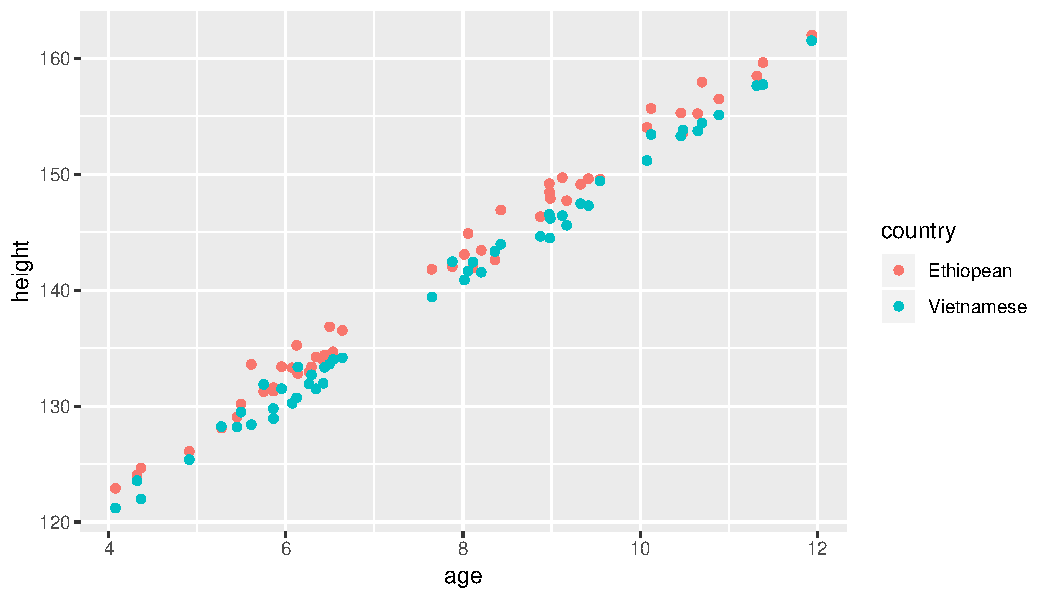
\includegraphics[width=\maxwidth]{figure/fig14-1} 

}


\begin{kframe}\begin{verbatim}
## 
## Call:
## lm(formula = height ~ age + country + age * country, data = data)
## 
## Residuals:
##     Min      1Q  Median      3Q     Max 
## -1.9692 -0.7366 -0.1769  0.6061  2.8313 
## 
## Coefficients:
##                        Estimate Std. Error t value Pr(>|t|)    
## (Intercept)           102.57196    0.53708 190.981   <2e-16 ***
## age                     5.02598    0.06686  75.168   <2e-16 ***
## countryVietnamese      -1.57419    0.75954  -2.073   0.0409 *  
## age:countryVietnamese  -0.01771    0.09456  -0.187   0.8518    
## ---
## Signif. codes:  0 '***' 0.001 '**' 0.01 '*' 0.05 '.' 0.1 ' ' 1
## 
## Residual standard error: 0.988 on 96 degrees of freedom
## Multiple R-squared:  0.9916,	Adjusted R-squared:  0.9913 
## F-statistic:  3779 on 3 and 96 DF,  p-value: < 2.2e-16
\end{verbatim}
\end{kframe}
\end{knitrout}

From this graph, we see that heights are similar because of age: older children are taller than younger children. But we also see that children are similar because of their national background: Ehtiopian children are systematically taller than Vietnamese children, irrespective of age. So here we see that a simple regression of height on age is not a good model. We see that when we estimate the simple regression on age and look at the residuals:

\begin{knitrout}
\definecolor{shadecolor}{rgb}{0.969, 0.969, 0.969}\color{fgcolor}

{\centering 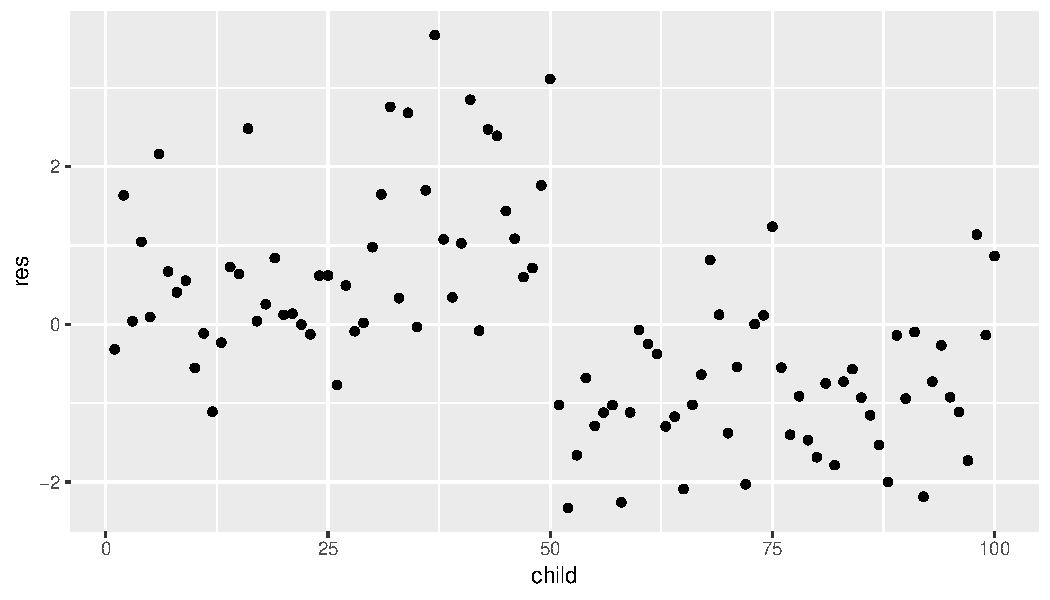
\includegraphics[width=\maxwidth]{figure/fig141-1} 

}



\end{knitrout}

As our model predicts random residuals, we expect a random scatter of residuals. However, what we see here is a systematic order in the residuals: they tend to be positive for the first 50 children and negative for the last 50 children. These turn out to be the Ethiopean and the Vietnamese children, respectively. This systematic order in the residuals is a violations of independence: the residuals should be random, and they are not. The residuals are dependent on country: positive for Ethiopeans, negative for Vietnamese children. Thus, there is more than just age that makes children similar. 
If we use multiple regression, including both age and country, we get the following regression equation:



\begin{eqnarray}
height = 102.641 + 5.017 \times age - 1.712 \times country + e
\end{eqnarray}

When we now plot the residuals we get a nice random scatter:

\begin{knitrout}
\definecolor{shadecolor}{rgb}{0.969, 0.969, 0.969}\color{fgcolor}

{\centering 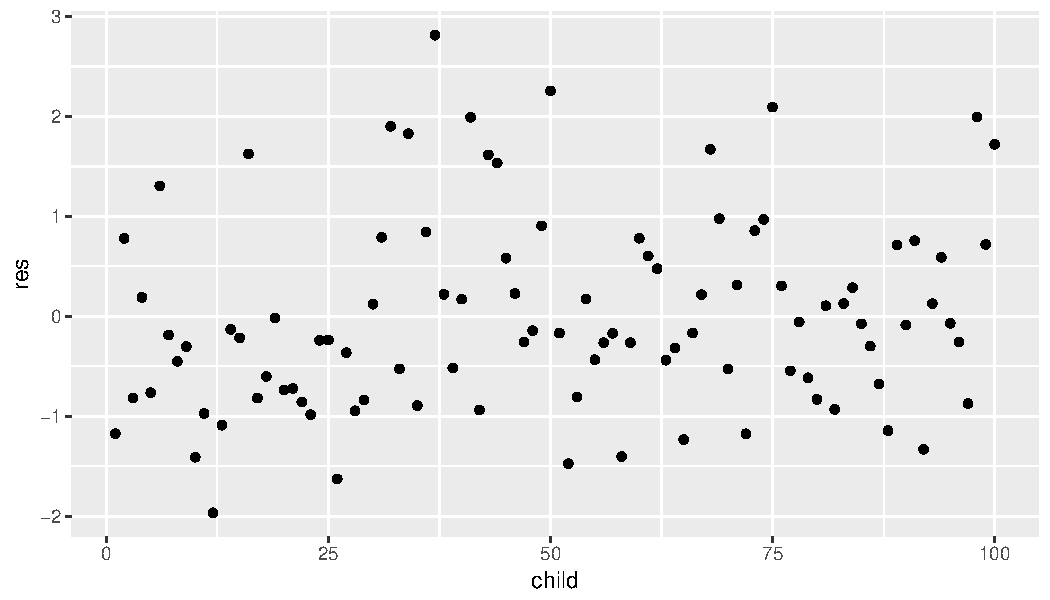
\includegraphics[width=\maxwidth]{figure/fig18888-1} 

}



\end{knitrout}


Another typical example of non random scatter of residuals is the following:

\begin{knitrout}
\definecolor{shadecolor}{rgb}{0.969, 0.969, 0.969}\color{fgcolor}

{\centering 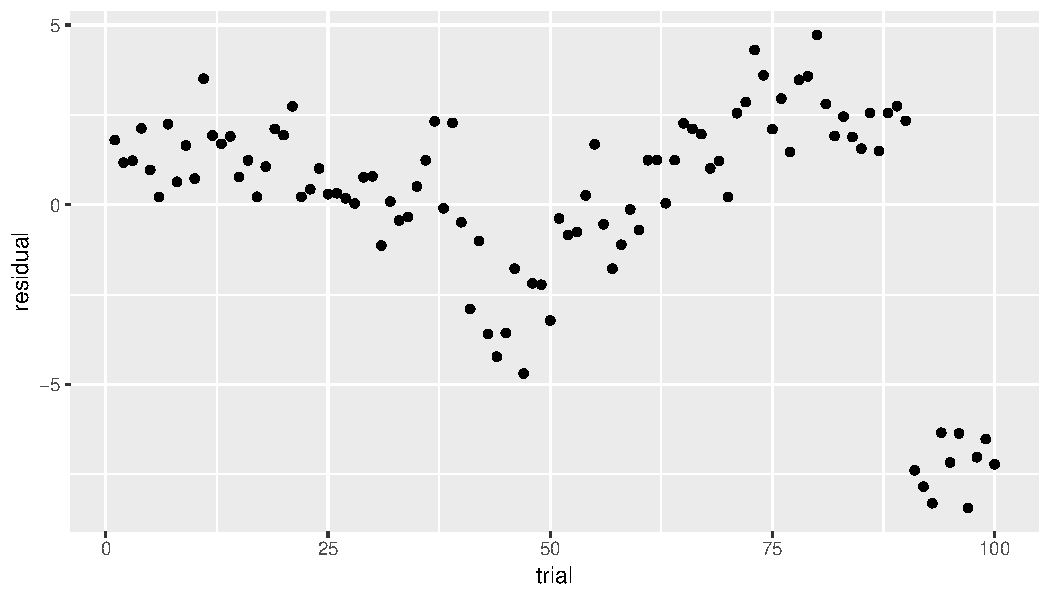
\includegraphics[width=\maxwidth]{figure/fig1413-1} 

}



\end{knitrout}

They come from an analysis of reaction times, done on 10 students where we also measured their IQ. Each student was measured on 10 trials. We predicted reaction time on the basis of student's IQ using a simple regression analysis. The residuals are clearly not random, and if we look more closely, we see some clustering if we give different colours for the data from the different students:


\begin{knitrout}
\definecolor{shadecolor}{rgb}{0.969, 0.969, 0.969}\color{fgcolor}

{\centering 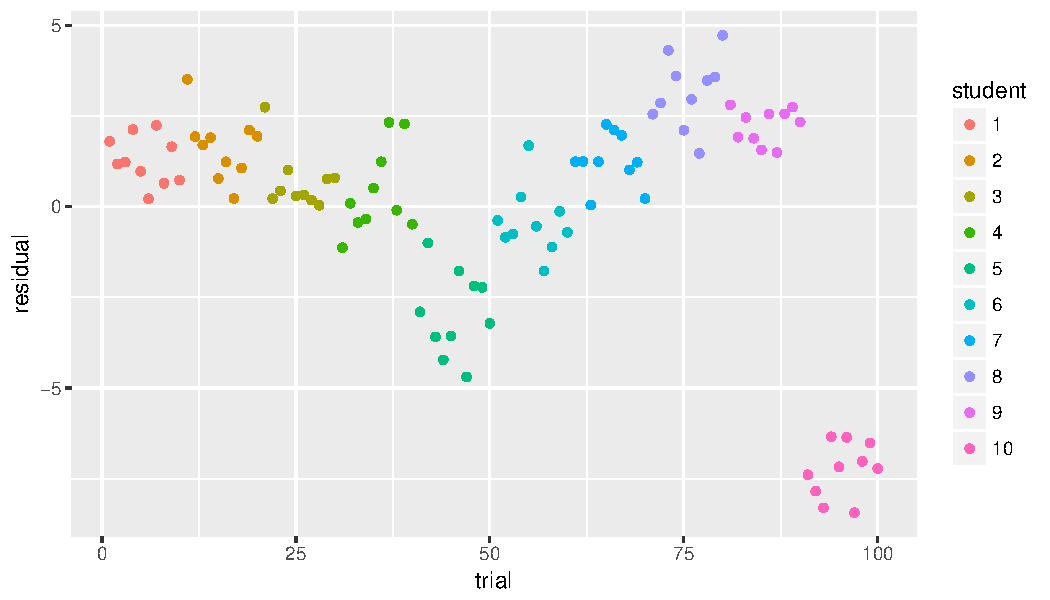
\includegraphics[width=\maxwidth]{figure/fig1415-1} 

}




{\centering 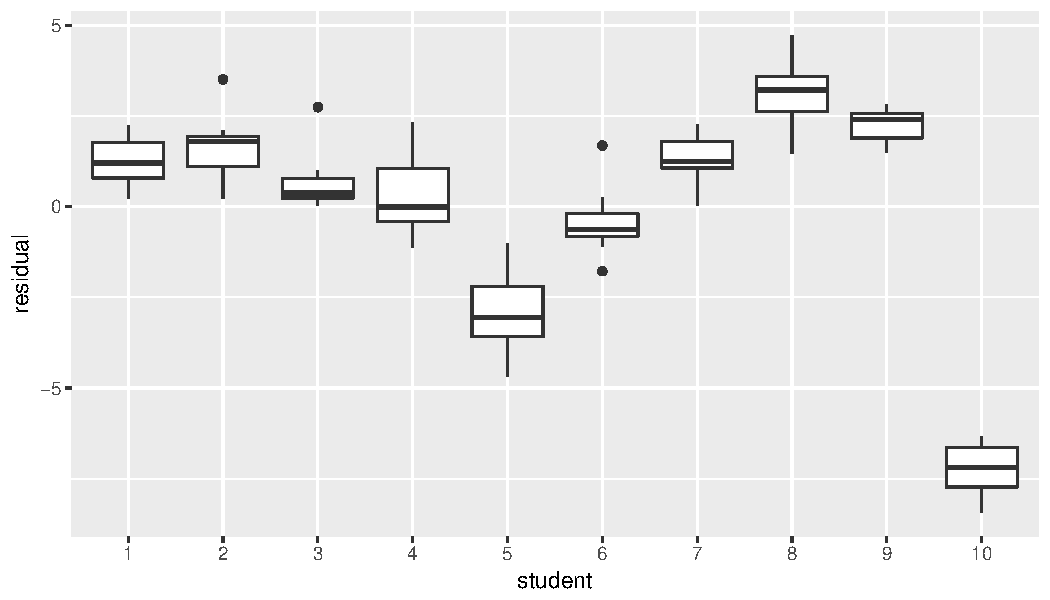
\includegraphics[width=\maxwidth]{figure/fig1415-2} 

}



\end{knitrout}

We see that residuals that are close toghether come from the same student. So, reaction time are not only similar because of IQ, but also because they come from the same student: clearly something else other than IQ explains why reaction times are dissimilar across individuals. The residuals in this analysis are not independent given IQ, they are dependent on the student. Thus, the assumption of independently distributed residuals is violated. 




\subsection{Linearity (additivity)}
\subsection{Homogeneity of variance}
\subsection{Residuals normally distributed}

\section{Testing assumptions}
\subsection{Independence}

Check the residuals, do you see any regularities? More specifically: Do you see any clustering? 

\subsection{Linearity (additivity)}
\subsection{Homogeneity of variance}
\subsection{Residuals normally distributed}

Make a histogram of the residuals: is the shape symmetric or skew? Is it more or less bell-shaped? Note that for small data sets, the shape is never perfectly normal. It should however have one peak and be symmetric.

\subsection{What to do when assumptions are violated?}

When the assumption of independence is violated, try including more predictors in your regression model. Like in the example of height in children, adding country into the equation solved the problem. In the case of reaction times, it was not clear what explains the clustering of residuals: we only know that reaction times from the same person were very similar. In such situations, consider linear \textit{mixed} models, to be discussed in a later chapter, and include a so-called \textit{random factor}, in this case for students. 



\subsection{nonlinearity}
If we have data and we analyze these with a linear (mixed) model, we can find nonlinearity. In that case we might introduce a quadratic term to make it more linear. For example, suppose we have the following data set, summarized in a scatter plot:

\begin{knitrout}
\definecolor{shadecolor}{rgb}{0.969, 0.969, 0.969}\color{fgcolor}

{\centering 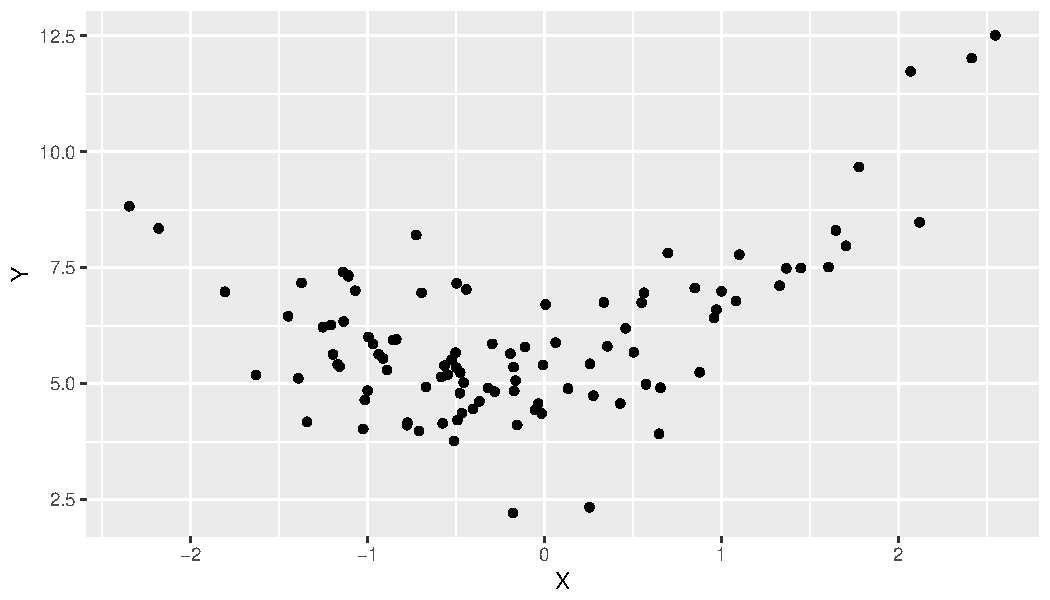
\includegraphics[width=\maxwidth]{figure/nonpar1-1} 

}



\end{knitrout}


We might then fit the following linear model, and find that it does not fit the data well:

\begin{equation}
y = b_0 + b_1 X + e 
\end{equation}

\begin{knitrout}
\definecolor{shadecolor}{rgb}{0.969, 0.969, 0.969}\color{fgcolor}

{\centering 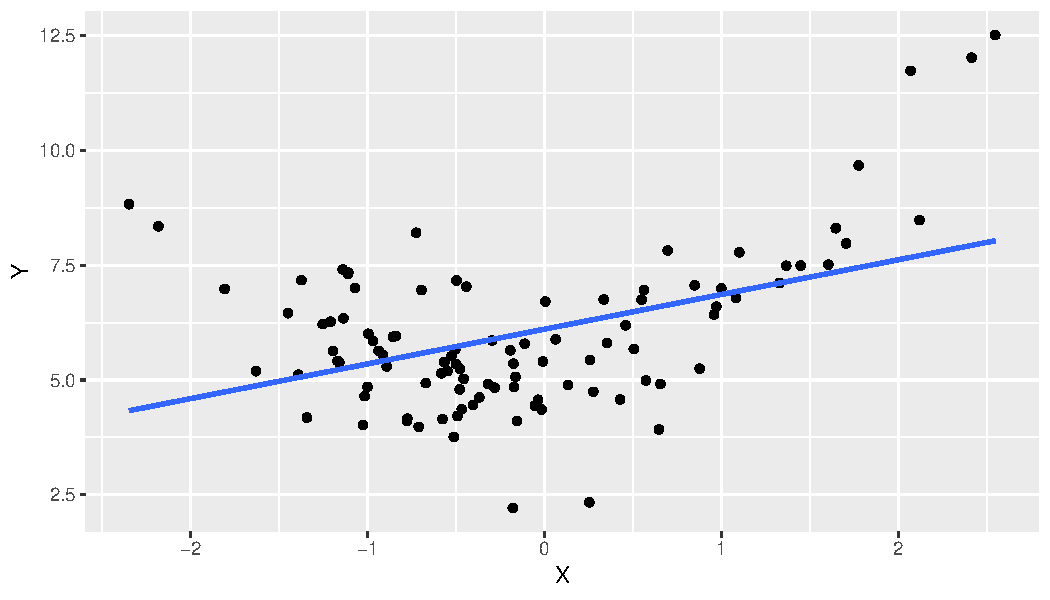
\includegraphics[width=\maxwidth]{figure/nonpar2-1} 

}



\end{knitrout}

A better model might be gained by introducing a new variable $X2$ that is computed by multiplying variable $X$ by itself: $X2=X^2$, and use this as an extra predictor:

\begin{equation}
y = b_0 + b_1 X + b_2 X2 + e 
\end{equation}


% <<ass1, fig.height=4, echo=FALSE, fig.align='center'>>=
% % dat2 <- data %>% mutate(X2 = X*X   )
% %        dat2   + ggplot( aes(X, Y) ) + geom_point() + geom_smooth(method=lm, se=F, formula= Y~ X+ X2)
% % 
% % 
% % names()
% @

 % assumptions


\chapter{Linear modelling: more advanced topics}


\subsection{Planned comparisons}

Suppose you have height data from three countries: Italy, Greece, and Norway. You might wish to know whether in these populations there is a difference in average height. If that is all you want to know, you can perform the SPSS UNIANOVA analysis described above. In that case, the null-hypothesis is
\\
\\
$H_0: \mu_{Italy}=\mu_{Greece}=\mu_{Norway}$
\\
\\
However, suppose your most important hypothesis is really much more specific: you only want to know whether the average height is different in Italy than in Greece. The corresponding hypothesis would then be: 
\\
\\
$H_0: \mu_{Italy}=\mu_{Greece}$
\\
\\
In such cases, where the null-hypothesis is more specific than simply stating "there are differences", then you should perform \textit{planned comparisons}. Here you would like to make a comparison between the average heights of Italy and Greece. You could also say you'd like to \textit{contrast} the average height of Italy with that of Greece. 

We then have to define this contrast in such a way that SPSS knows what we want. So we could define our contrast in a similar vein as the null-hypothesis. Let's call the contrast $\gamma_1$.
\\
\\
$\gamma_1: \mu_{Italy}=\mu_{Greece}$
\\
\\

This contrast could also be written such that there is zero on the right-hand side of the equation, like this:
\\
\\
$\gamma_1: \mu_{Italy}-\mu_{Greece}=0$
\\
\\
This is the preferred way of specifying contrasts: having a zero on the right-hand side. And how about Norway? How do we add Norway into this contrast? Well, notice that you could also write the contrast like this:
\\
\\
$\gamma_1: (1)\times \mu_{Italy} + (-1) \times \mu_{Greece} + (0) \times \mu_{Norway} =0$
\\
\\
So we could code this specific contrast with the numbers preceding the group means: A 1 for Italy, a -1 for Greece and a 0 for Norway. For SPSS therefore, to specify a contrast, we only need this coding. This can be done in the following way. Suppose you have the following data on height, summarized in a boxplot:


\begin{knitrout}
\definecolor{shadecolor}{rgb}{0.969, 0.969, 0.969}\color{fgcolor}

{\centering 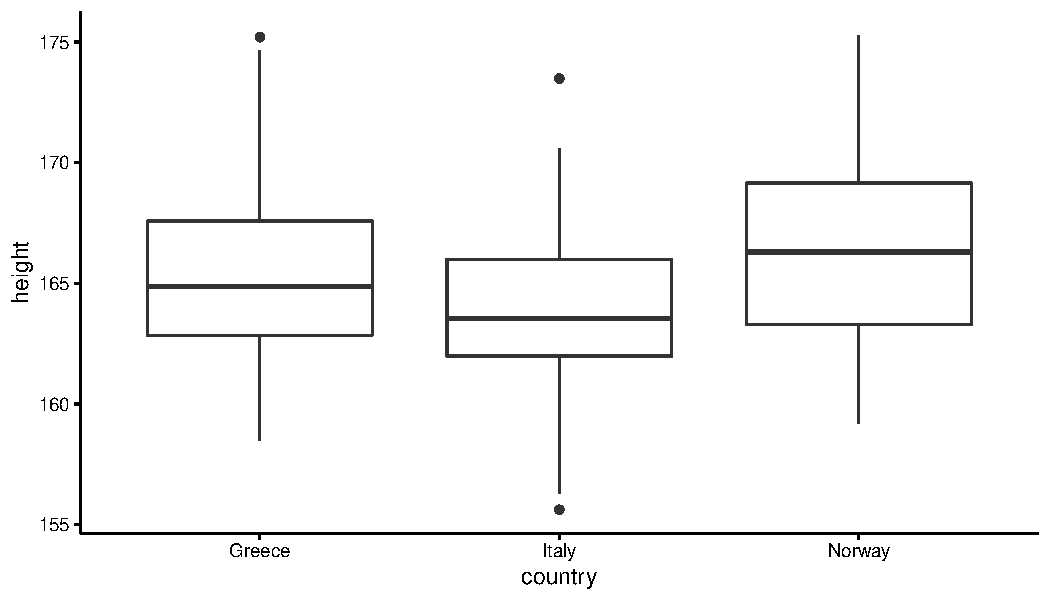
\includegraphics[width=\maxwidth]{figure/fig1416-1} 

}



\end{knitrout}

Note that in this data set, group 1 is Greece, group 2 is Italy and group 3 is Norway. Then we could use the following syntax to ask for the specific comparison (or contrast) of the first and the second group, that is, Greece and Italy, respectively. So group 1 (=Greece) gets a -1, group 2 (=Italy) gets a 1, and group 3 (=Norway) gets a 0, so our coded contrast looks like $(-1, 1, 0)$.

\begin{verbatim}
UNIANOVA height BY country
/DESIGN=country
/CONTRAST(country)=SPECIAL(-1  1  0).
\end{verbatim}

Below we see the output:
\begin{figure}[h]
    \begin{center}
       \includegraphics[scale=0.4,trim={0cm 0cm 0cm 2cm}, clip,width=0.7\linewidth]{/Users/stephanievandenberg/Dropbox/Statistiek_Onderwijs/Data" "Analysis/spss" "examples" "linear" "model/planned" "comparisons/plannedcontrast1.png}
    \end{center}
\end{figure}

From the output, we see first see that the general null-hypothesis that all three countries have the same average height is rejected, $F(2, 147)= 6.14, MSE=14.77, p = 0.003$. This test has 2 degrees of freedom, one for each of the two dummy variables that are needed to test this model. The error degrees of freedom equals 147: that is the number of data points (300) minus the number of parameters in the model: one for the intercept and two for the dummy variables, so $300-3=247$.

Next, we see the results for our \textit{specific} null-hypothesis: that the means for Greece and Italy are equal, irrespective of Norway. We see a Contrast Estimate of -1.008 and a significance level of $p=0.19$. So the contrast is negative: what does this mean? Well, let's put the -1.008 into our contrast above:
\\
\\
$\gamma_1: (1)\times \mu_{Italy} + (-1) \times \mu_{Greece} + (0) \times \mu_{Norway} = -1.008$
\\
\\
which can be simplified to
\\
\\
$\gamma_1:  \mu_{Italy}   =  \mu_{Greece} - 1.008$
\\
\\
So the -1.008 indicates that the average height in Italy is 1.008 cm shorter than in Greece, at least in our sample. The relatively high $p$-value indicates that the population means are however not different: we do not reject the null-hypothesis that the average heights are the same.
We also see an $F$-test for this contrast, $F(1, 147)=1.721, MSE= 14.76, p=0.19$.
Since the first degrees of freedom number is a 1, we know that $F$ is the same as a squared $t$, $t^2$, So, an equivalent presentation of the contrast effect would be $t(147)=2.96, p=0.19$

Now perhaps you realize, why didn't we do a $t$-test in the first place? We might have taken the Greece and Italy data separately, used a dummy variable and then run an ordinary linear model. Well, let's see what would happen then.
First we let SPSS select only the Italy and Greece data with the SELECT IF syntax, and next run an UNIANOVA, using the BY keyword for country to indicate that we treat it as a qualitative variable. We also let the selection be preceded by a TEMPORARY commmand, to indicate that the selection only applies to the analysis that follows.

\begin{verbatim}
TEMPORARY.
SELECT IF (country<3).
UNIANOVA height BY country
/DESIGN=country
/PRINT = PARAMETER.  
\end{verbatim}


Below we see the output:
\begin{figure}[h]
    \begin{center}
       \includegraphics[scale=0.4]{/Users/stephanievandenberg/Dropbox/Statistiek_Onderwijs/Data" "Analysis/spss" "examples" "linear" "model/planned" "comparisons/simplettest.png}
    \end{center}
\end{figure}

We see that now only the data from Greece and Italy are compared. From the Parameter Estimates table, we see that country 2 is the reference category, which is Italy. We also see that the average height in Greece is 1.008 cm taller than Italy. This effect is not significant, $t(98)=1.371,p=0.17$. We use 98 degrees of freedom because we have 100 people and loose 2 degrees of freedom, one for the intercept and once for the regression coefficient for country=1. Note that this number is also indicated in the Tests of Between-Subjects Effects table, as the df of the Error. 

So what is different from the contrast effect? First of all, we see that the $p$-value is different: the $p$-value for the contrast effect analysis is somewhat larger than the one for the 'ordinary' $t$-test. Second, we see that the $t$-statistic is different: In the contrast analysis the $t$-value was 2.96 and in the ordinary analysis it was 1.371. So part of the reason that the $p$-value is different for the contrast is that the $t$-value is higher. Third, we see that the degrees of freedom has changed from 147 to 98. Well, we know that the significance level of a $t$-value depends on its size, the higher the $t$-value the lower the $p$-value, and we know that significance also depends on the degrees of freedom: the more degrees of freedom, the lower the $p$-value. 

So why has the $t$-value changed? Well, we know that the $t$-value is nothing but the regression coefficient divided by its standard error, $t=B/{SE}$. If we compare the two outputs, we see that the effect of $B$ is the same, the regression coefficient is equal to 1.008, and the contrast estimate in the Contrast Results (K-Matrix) is -1.008. So the sizes are the same, even if the sign is different. 

So the only difference between the two analyses can be the standard error. It turns out the standard error is computed in different ways: in the first contrast analysis, this SE is computed on the basis of \textit{all} the data, including the Norway data. We can see that from the degrees of freedom, the number of people minus 3. Why three? Because we also compute the variance of the Norway data, for which we have to estimate the mean (variance is the average squared difference from the mean). In the second analysis, we only used the data from 100 Greeks and Italians. The Norway data was not used at all, that's why the degrees of freedom is different and also the standard error for our $t$-statistic. 
\\
\\
Thus in summary: if we have a very specific hypothesis about the difference in means among two groups, it gives more statistical power to use a contrast analysis, rather than a simple analysis regarding only those two groups. The reason for this increase in power is that more information is used, even from groups for which we have no specific hypothesis. 
\\
Note that here we saw a higher $p$-value for the contrast analysis, but still, in general it is wiser to use as much data as possible, so we prefer a contrast analysis over a simple analysis excluding other groups.
\\
\\
The above example of comparing only the means of two groups, at the same time making use of the data in other groups, is called a \textit{simple contrast}. Now let's look at a \textit{complex contrast}. Suppose your hypothesis is that average height is different in Northern-European countries than in Southern-European countries, then you would like to know whether Italy AND Greece taken together differ regarding the average height from Norway. So we'd like to compare the average height in Norway to the average height in Greece and Italy together. We could write that null-hypothesis as follows:

\begin{eqnarray}
H_0 : \mu_{Norway} = \frac{\mu_{Greece}+ \mu_{Italy}}{2}
\end{eqnarray}


In other words, the mean height in Norway is equal to the \textit{average} mean height in the two other countries. If we want to test this hypothesis, we have to define a contrast. So if we divide the means of Greece and Italy by 2, we can compare their sum to the mean of Norway. We could write the contrast in the following way:

\begin{eqnarray}
\gamma_2 : \mu_{Norway} - \frac{\mu_{Greece}}{2} - \frac{\mu_{Italy}}{2} = 0 
\end{eqnarray}

or, equivalently, like this:

\begin{eqnarray}
\gamma_2 : \mu_{Norway} - \frac{1}{2}  \mu_{Greece} - \frac{1}{2}  \mu_{Italy} = 0 
\end{eqnarray}


In SPSS, we can code this in the following way $(1  -\frac{1}{2} -\frac{1}{2})$. But because the countries have a different order in our data (1=Greece, 2=Italy, 3=Norway), we use the following syntax:

\begin{verbatim}
UNIANOVA height BY country
/DESIGN=country
/CONTRAST(country)=SPECIAL(-0.5  -0.5  1).
\end{verbatim}


Now let's compare this analysis where we use a dummy variable NrthrnEr, where we code 1s for Norwegians and 0s for Greeks and Italians. We then run an ordinary linear model on the data using this dummy has a predictor quantitatively:


\begin{verbatim}
UNIANOVA height WITH NrthrnEr
/PRINT=PARAMETER
/DESIGN=NrthrnEr.
\end{verbatim}

From the contrast analysis we obtain $F(1,147)=10.56, MSE=14.77, p=0.001$, which is equivalent to $t(147)=3.25, p=0.001$. From the dummy variable analysis, we obtain $t(148)= 3.24, p=0.001$. So in this case, the results are very close: the degrees of freedom is larger for the dummy variable analysis, but the $t$-value is lower. All in all, we gain nothing much, and that is because in the dummy analysis we also use all of the data: we put the Greeks and Italians in one group (N=100), and the Norwegians in another group (N=50). The degrees of freedom therefore differs cause we only need to estimate 2 means in the dummy analysis, instead of 3 in the contrast analysis.

In general: if you run a model where you compare various groups, AND you have very specific hypotheses that you'd like to test, it is generally advised to run a contrast analysis, including a small number of them, and then report only the tests and $p$-values of those contrast. Do not then also report the $p$-values of the parameters of your model. Actually, your contrasts are a respecification of your model: either report the contrasts or the parameters, but not both, since they contain the same information. If you report too many $p$-values, the probability that you make a Type I error (concluding that you have a significant difference while there is really no difference) becomes too large. That is also the reason why you should report not more contrasts than the number of your parameters for your variable. For example, if you compare 5 groups, you will have 4 parameters for these groups. In that case specify no more than 4 contrasts. SPSS has a number of prespecified sets of contrasts, like Helmert, Deviation, Difference, etcetera. Check out the SPSS manual for more details. If you want something more specific, use the SPECIAL option as indicated above. 

Also very important: only go for contrasts when the overall ANOVA is significant. If the group means are not significantly different from eachother in a general sense, it is generally not advised to test specific contrasts.

\subsection{Testing more than one contrast}

In some cases you have a number of research hypotheses about group differences. For instance, you might have the a priori hypothesis that people in Northern countries are taller than in Southern countries, and another a priori hypothesis that people in Western countries are taller than in Eastern countries. So, a priori you have the hypothesis that the mean height in Norway is different from the mean heights in Greece and Italy combined. Second, you expect that the mean height in Italy is higher than in Greece.

You could test these two hypotheses at once in SPSS by specifying a $K$ matrix, like so:

\begin{verbatim}
UNIANOVA height BY country
/DESIGN=country
/CONTRAST(country)=SPECIAL(-0.5  -0.5  1
                            1 -1   0).
\end{verbatim}

Remember that the countries were coded like 1=Greece, 2=Italy, and 3= Norway. So the first null-hypothesis that is tested is that Norway has the same mean as the average of Greece and Italy. The second null-hypothesis is that Greece and Italy have the same mean.

This set of contrasts is said to be \textit{orthogonal}: whether or not we find a significant result for the first contrast has nothing to do with whether we find a significant result for the second contrast. Why this is the case can be seen from the $K$ matrix: if we take the first elements of the first and second row and multiply them we get $-0.5 \times 1 = -0.5$. If we take the second elements of the first and second row and multiply them we get $-0.5 \times -1 = 0.5$. If we take the third elements of the first and second row and multiply them we get $1 \times 0 = 0$. If we add these numbers we get $-0.5 + 0.5 +0= 0 $. Here we get a total of 0, which indicates that the contrasts are orthogonal, implying that the statistical results for contrast 1 and 2 are independent of eachother. If the sum is unequal to 0, the contrasts are said to be \textit{dependent}. 
Here's an example of a non-orthogonal set of contrasts:

\begin{verbatim}
UNIANOVA height BY country
/DESIGN=country
/CONTRAST(country)=SPECIAL(1  0  -1
                            1 -1   0).
\end{verbatim}

Here the sum of the products equals $1\times 1 +0\times -1 + -1 \times 0 =1$. This means that the set of statistical results is not independent of each other, so if the null-hypothesis if the first contrast is significant, this yields some information about the probablity of obtaining a significant result for the second contrast. This you do not want, of course. So generally you would want to use independent sets of contrast. However, research questions are always more important: if you have good theoretical reason to specify a set of non-orthogonal contrast, just go for it (Stevens, ).

As stated earlier, SPSS has a number of pre-specified sets of contrasts. One of them is the Helmert contrast. In the Helmert contrast, the first group is contrasted with the average of all later groups, the second group is compared to the average of the later groups (ignoring group 1), the third group is compared with the average of the later groups (ignoring groups 1 and 2), etcetera. For a five country analysis, the syntax would be like


\begin{verbatim}
UNIANOVA height BY country
/DESIGN=country
/CONTRAST(country)=SPECIAL(1     -0.25 -0.25 -0.25 -0.25
                            0 1 -0.33 -0.33 -0.33
                            0 0 1 -0.5 -0.5
                            0 0 0 1 -1).
\end{verbatim}

and this is equivalent to the syntax 

\begin{verbatim}
UNIANOVA height BY country
/DESIGN=country
/CONTRAST(country)=HELMERT.
\end{verbatim}


This set of 4 contrasts is also completely orthogonal: all pairs of contrasts are orthogonal.





\subsection{Post-hoc comparisons}

In some cases, you compare 3 or more groups, and you find some interesting differences. For instance, in the above example, when you look at the boxplot of the  differences between Norway, Greece and Italy, you might wonder whether there is a real difference in Italy and Greece. Or perhaps there is a difference between Norway and Italy, or even between Norway and Greece. There might be all kinds of interesting things to find out from these data.
In this case note, that we now formulate these hypotheses \textit{after} looking at the difference in our data. In this case, suppose that there were not specific hypothesis before collecting our data, that we merely wanted to find out whether there are differences between mean heights across these countries. So, our null-hypothesis before looking at the data was that there were no differences in mean height across Greek, Italian and Norwegian populations. To test this we perform a regular linear model analysis, with height as the dependent variable and a categorical variable country as independent variable. We want SPSS to make dummy variables automatically, so we use the following syntax using BY:

\begin{verbatim}
UNIANOVA height BY country
/PRINT=PARAMETER
/DESIGN=country.
\end{verbatim}



\begin{figure}[h]
    \begin{center}
       \includegraphics[scale=0.8,trim={0cm 22cm 0cm 2cm}, clip,width=0.7\linewidth]{/Users/stephanievandenberg/Dropbox/Statistiek_Onderwijs/Data" "Analysis/spss" "examples" "linear" "model/posthoc" "comparisons/Ftest}
    \end{center}
\end{figure}


From the output we use the $F$-test to test the overall hypothesis about equality of means, and report a significant difference between the three means, $F(2, 147)=6.14 , MSE=14.77, p<0.05$. Now \textit{given} that we have this rejection of the null-hypothesis, we might be very interested where this significance comes from: is it that Norway is very different from the other two countries? Perhaps there are no differences between Greece and Italy? Perhaps there is only a real difference between Norway
and Italy, but no real difference between Greece and Italy. And so on, and so forth. Note that here you could make 3 pair-wise comparisons: Greece vs Italy, Greece vs Norway and Italy vs Norway. You or anyone else intested in your research would like to know if these pair-wise differences are significant. In that case you can report so-called post hoc pairwise comparisons. 

Note that we do not perform planned comparisons using contrasts here. Planned comparisons are very powerful tools that are only allowed for hypotheses that are specificied a priori, that is, before doing any analysis, and preferably before any data collection. Post hoc comparisons are done after the fact: after testing the research hypothesis and after having looked at the data (seeing means or boxplots!), you can test extra hypotheses that are of secondary interest. First we will show you how to do it, and second we will explain why we do it like that. 

\begin{verbatim}
UNIANOVA height BY country
/PRINT=PARAMETER
/DESIGN=country
/POSTHOC=country(BONFERRONI).
\end{verbatim}

So we state that we wish to see posthoc comparisons for the variable \textit{country}. In parentheses we indicate \textit{Bonferroni}, which we will explain later.

\begin{figure}[h]
    \begin{center}
       \includegraphics[scale=0.8,trim={0cm 20cm 0cm 2cm}, clip,width=0.7\linewidth]{/Users/stephanievandenberg/Dropbox/Statistiek_Onderwijs/Data" "Analysis/spss" "examples" "linear" "model/posthoc" "comparisons/Posthoctest}
    \end{center}
\end{figure}

From the figure we see that there are 6 comparisons, but by closer inspection we see that all three possible comparisons are reported twice. We see a significant difference between Italy and Norway, $p<0.002$, and that the other two comparisons are not significant. So average height in Greece is not different from the average height in Italy, $p>0.575$, nor from that in Norway, $p>0.097$.
Now note the difference from the Planned comparisons analysis. There we found a p-value of 0.19 for the hypothesis that Greece has the same average height as Italy. This contrast had a somewhat higher p-value than a simple dummy analysis for Greece and Italy, ignoring the Norwegian data, p=0.17. And now we see a much higher p-value of 0.58. The reason is that a correction has been applied to the p-values. This correction is needed because otherwise we too easily conclude that there are true differences between Greece and Italy.

Remember that the probability of a Type I error is very often chosen to be $5\%$. If we have one nullhypothesis that we want to test, the probability that we incorrectly conclude that there \textit{is} a difference in means (but there is really \textit{no} difference at population level!) is $5\%$. But suppose we have 10 hypotheses that we wish to test. Then what is the probability of finding at least 1 signficant result while there is no difference? Well, it could be that our first hypothesis is falsely rejected, or our second, or our third, or perhaps even both our second and fourth hypothesis, and so on and so forth. With 10 hypotheses to test, there will be a high probablity that at least 1 will be falsely rejected. If \textit{each} hypothesis has a probability of a Type I error of 5\%, the probability that none of the hypotheses is falsely rejected equals $0.95^10=0.60$ (if we assume that all probablities are independent). So the probability that at least one is falsely rejected is the complement of that, so 0.40. So if we carry out such research with 10 hypotheses, each using a significance level of $5\%$, we actually have a probability of 40\% of making at least one Type I error! That is awful, we don't want that. That's why in research, with a lot of hypotheses to be tested, we generally adjust the p-value in order to be more careful rejecting null-hypotheses. So theoretically, the p-value of our posthoc comparison of Greece and Italy should be equal to 0.19, corresponding to the simple dummy variable analysis ignoring Norway, but we report 0.575, because we also test two other hypotheses here. Actually, the $p$-value of the simple analysis of 0.19 is multiplied by the total number of tests, which is 3.


\subsection{Posthoc tests for complex contrasts}



\subsection{Fishing expeditions}
The practice of testing a lot of hypotheses is often described as a fishing expedition. Just set out with large nets, throw them out, and catch whatever you can. In some extreme cases, in genetics for example, researchers test thousands or even millions of hypotheses on the basis of only one data set. Imagine that you collect height data on 70 countries and you want to know what countries differ from what other countries. The total number of pairs of countries equals 70 over 2, which is equal to 2415. So with 2415 p-values, what is the a priori probablity of a significant result? If in reality there ARE no differences in means, and a fixed significance level of 0.05, 5\% of the p-values will be significant! So with such a data set, there will be at least $0.05 \times 2415 = 121$ significant p-values. At least, because there might be some true ones too. So in that scenario, it is impossible to know which p-values are too be trusted: many of them will involve false rejections.

For this reason, always be very specific about the null-hypothesis that you want to test with your data. If you have a very specific hypothesis about the differences in means, following a specific pattern, then always use a planned contrasts analysis. If after your analysis, there are some secondary hypotheses that you'd like to check (but for which you had no specific expectation) then report posthoc tests. The Bonferroni post hoc test is a good choice, as it is very conservative: it is very unlikely that you will falsely reject a hypothesis. Alternatively, there are some other post hoc tests, for further reading see the SPSS manual.

In general do a contrast analysis (planned comparisons) if:


\begin{itemize}
\item the overall test for the equality of all means is significant
\item the comparisons are chosen \textit{before} looking at the results (means, plots, statistical tests): they should be planned ahead!
\item the number of planned contrasts should not exceed the degrees of freedom, that is, the number of groups minus 1. 
\end{itemize}


Otherwise, do posthoc analyses, or better still, perform as few tests as possible! Only do posthoc tests if you are in an exploratory mood (you're not having a specific hypothesis but you would like to get some new ideas for future research) or when your supervisor asks for them.





\subsubsection{Exercises}

You compare 4 groups. You'd like to know whether the averages observed in groups 1 and 2 differ from the averages observed in groups 3 and 4. 

\begin{itemize}
\item State the null hypothesis
\item Define the contrast
\item Provide the SPSS syntax for this contrast
\end{itemize}

answers: 
\begin{itemize}
\item $H_0: \frac{\mu_1 + \mu_2}{2} - \frac{\mu_3 + \mu_4}{2} = 0  $
\item (0.5 0.5 -0.5 -0.5)
\item \begin{verbatim}
UNIANOVA height BY group
/DESIGN=country
/CONTRAST(country)=SPECIAL(0.5 0.5 -0.5 -0.5).
\end{verbatim}
\end{itemize}




You compare 5 groups. You'd like to know whether the average observed in group 1 differs from the averages observed in groups 3, 4 and 5. 

\begin{itemize}
\item State the null hypothesis
\item Define the contrast
\item Provide the SPSS syntax for this contrast
\end{itemize}

answers: 
\begin{itemize}
\item $H_0: \frac{\mu_1}{1} - \frac{\mu_3 + \mu_4 + \mu_5}{3} = 0  $
\item (1 0 -0.33 -0.33 -0.33)
\item \begin{verbatim}
UNIANOVA height BY group
/DESIGN=group
/CONTRAST(group)=SPECIAL((1 0 -0.33 -0.33 -0.33)).
\end{verbatim}
\end{itemize}


A student has run the following SPSS syntax:

\begin{verbatim}
UNIANOVA score BY school
/DESIGN=school
/CONTRAST(school)=SPECIAL((0 0 1 -0.5 -0.5)).
\end{verbatim}

What null-hypothesis is tested using this syntax?
\\
answer:
The hypothesis that the average score in school 3 is the same as the mean average score in schools 4 and 5
or 
$H_0: \mu_3 = \frac{\mu_4 + \mu_5}{2}$
\\
\\
A student has tested the research hypothesis that height is different in the Benelux countries: The Netherlands, Belgium and Luxemburg, and finds a significant result. His supervisor asks then where the differences come from: is it that height is different in the Netherlands, or is it perhaps Luxemburg that deviates from the other two countries? She would like to have more specific information where the differences are between these three countries. What would you advise this student to do?
\\
\\
answer: the supervisor does not seem to have any clearcut hypthesis about height differences in the Benelux countries. You therefore advise to carry a number of posthoc tests, that take into account the increase in the probability of a Type I error by adjusting p-values.
\\
\\
A student has tested the research hypothesis that height is different in the Benelux countries: The Netherlands, Belgium and Luxemburg, and finds a significant result. His supervisor then says that the student is not finished yet. She would like to know whether the theory is correct that the larger the country, the taller the people. She would therefore like to know whether the average height in small country Luxemburg is different from the height averages in Belgium and The Netherlands.
\\
\\
answer: the supervisor has a clearcut hypothesis about height differences in the Benelux countries. You therefore advise to carry out a planned comparison (a contrast analysis), that specifically tests the null hypothesis that the average in Luxemburg is the same as the mean average of Belgium and the Netherlands together.


 % advanced topices linear models

\chapter{When assumptions are not met: non-parametric alternatives}



Linear models do not apply to every data set. As discussed before, sometimes the assumptions of linear modelling are not met. One of the assumptions is linearity or additivity. Additivity requires that one unit change in variable X leads to the same amount of change in Y, no matter what value X has. For bivariate relationships this leads to a linear shape. But sometimes you can only expect that Y will change in the same direction, but you don't believe that this amount is the same for all values of X. This is the case for example with ordinal dependent variable. Suppose we wish to model the relationship between age of the mother and an aggression score of her 7-year-old child. Suppose aggression is measured on a three-point ordinal scale: not aggressive, sometimes aggressive, often aggressive. Since we do not know the quantitative differences between these three levels there are many graphs we could draw for a given data set.


Suppose we have the following data set:


\begin{knitrout}
\definecolor{shadecolor}{rgb}{0.969, 0.969, 0.969}\color{fgcolor}
\begin{tabular}{r|l}
\hline
AgeMother & Aggression\\
\hline
32 & Sometimes aggressive\\
\hline
31 & Often aggressive\\
\hline
32 & Often aggressive\\
\hline
30 & Not aggressive\\
\hline
31 & Sometimes aggressive\\
\hline
30 & Sometimes aggressive\\
\hline
31 & Not aggressive\\
\hline
31 & Often aggressive\\
\hline
31 & Not aggressive\\
\hline
30 & Sometimes aggressive\\
\hline
32 & Often aggressive\\
\hline
32 & Often aggressive\\
\hline
31 & Sometimes aggressive\\
\hline
30 & Sometimes aggressive\\
\hline
31 & Not aggressive\\
\hline
\end{tabular}


\end{knitrout}

If we want to make a scatter plot, we could choose the values 1, 2, and 3 for the three categories respectively. We would then get the following plot:


\begin{knitrout}
\definecolor{shadecolor}{rgb}{0.969, 0.969, 0.969}\color{fgcolor}

{\centering 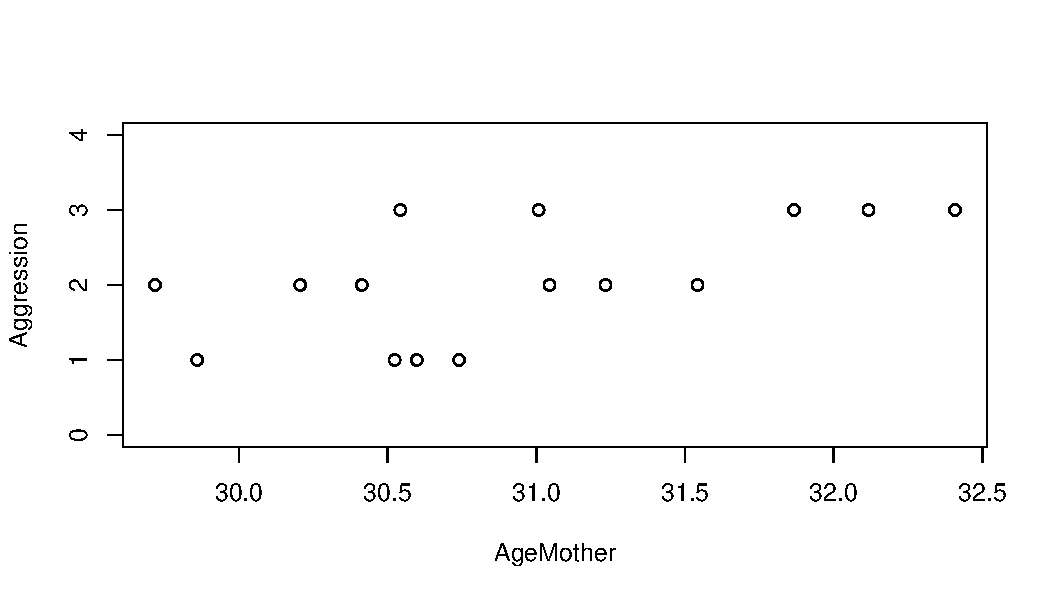
\includegraphics[width=\maxwidth]{figure/fig101-1} 

}



\end{knitrout}

But since the Aggression data are ordinal, we could also choose values 0, 2, and 3:

\begin{knitrout}
\definecolor{shadecolor}{rgb}{0.969, 0.969, 0.969}\color{fgcolor}

{\centering 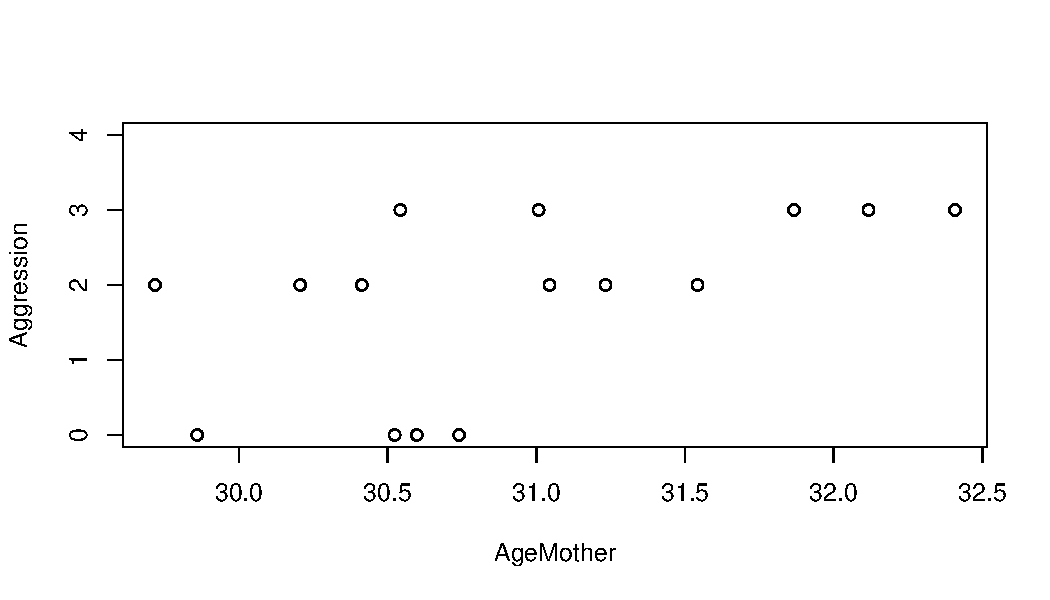
\includegraphics[width=\maxwidth]{figure/fig1114-1} 

}



\end{knitrout}

As we change the scale for the ordinal variable, we also see the best fitting regression line changing. 

So with ordinal data, the assumption of additivity is often not met, since the values for a quantitative analysis are arbitrarily chosen. 

In some case though, ordinal data could be modelled linearly. Look at the following example where we measured aggression with a 7-point Likert scale:


\begin{knitrout}
\definecolor{shadecolor}{rgb}{0.969, 0.969, 0.969}\color{fgcolor}
\begin{tabular}{r|r}
\hline
AgeMother & Aggression\\
\hline
35 & 6\\
\hline
32 & 4\\
\hline
35 & 6\\
\hline
36 & 5\\
\hline
33 & 3\\
\hline
30 & 1\\
\hline
32 & 4\\
\hline
32 & 2\\
\hline
34 & 4\\
\hline
30 & 2\\
\hline
32 & 3\\
\hline
31 & 2\\
\hline
32 & 3\\
\hline
31 & 3\\
\hline
38 & 7\\
\hline
\end{tabular}


\end{knitrout}

When we plot these data, using the values 1 through 7, we see a nice linear relationship. So even when the values are arbitrarily chosen, a linear model can be a good model for a given data set with ordinal variables. 

\begin{knitrout}
\definecolor{shadecolor}{rgb}{0.969, 0.969, 0.969}\color{fgcolor}

{\centering 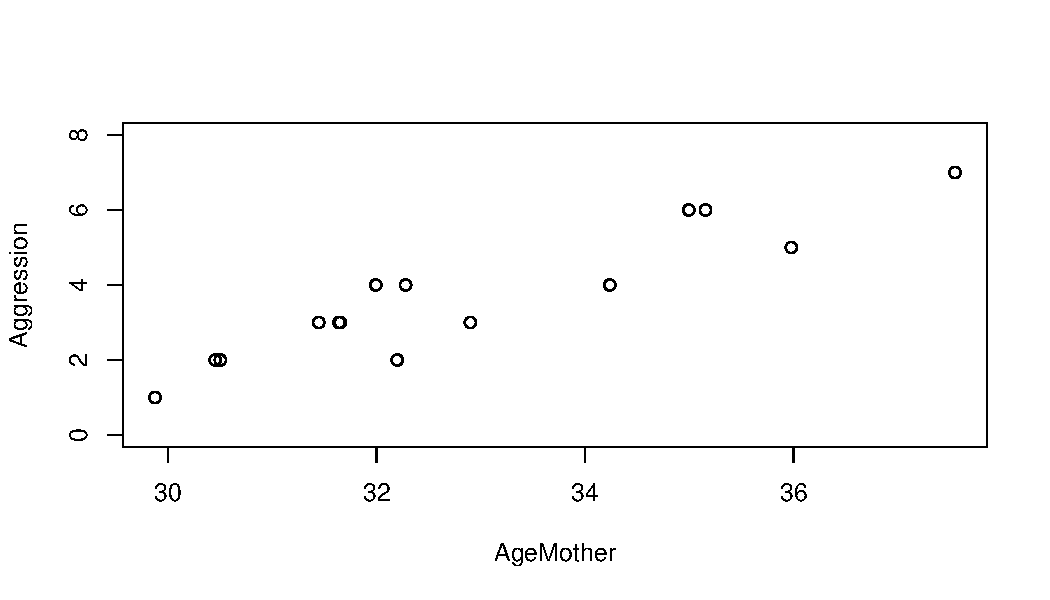
\includegraphics[width=\maxwidth]{figure/fig1121-1} 

}



\end{knitrout}

So with ordinal data, always check that your data indeed conform to a linear model, but realize at the same time that you're assuming a quantitative relationship between the variables that may or may not make sense. 

If you believe that a quantitative analysis is meaningless then consider nonparametric analysis. 

Another case where we favour a nonparameteric analysis, is when the assumption of normally distributed residuals is not tenable. For instance look again at Figure ????. When we perform a regression analysis and plot a histogram of the residuals, we see the following:

\begin{knitrout}
\definecolor{shadecolor}{rgb}{0.969, 0.969, 0.969}\color{fgcolor}\begin{kframe}


{\ttfamily\noindent\itshape\color{messagecolor}{\#\# `stat\_bin()` using `bins = 30`. Pick better value with `binwidth`.}}\end{kframe}

{\centering 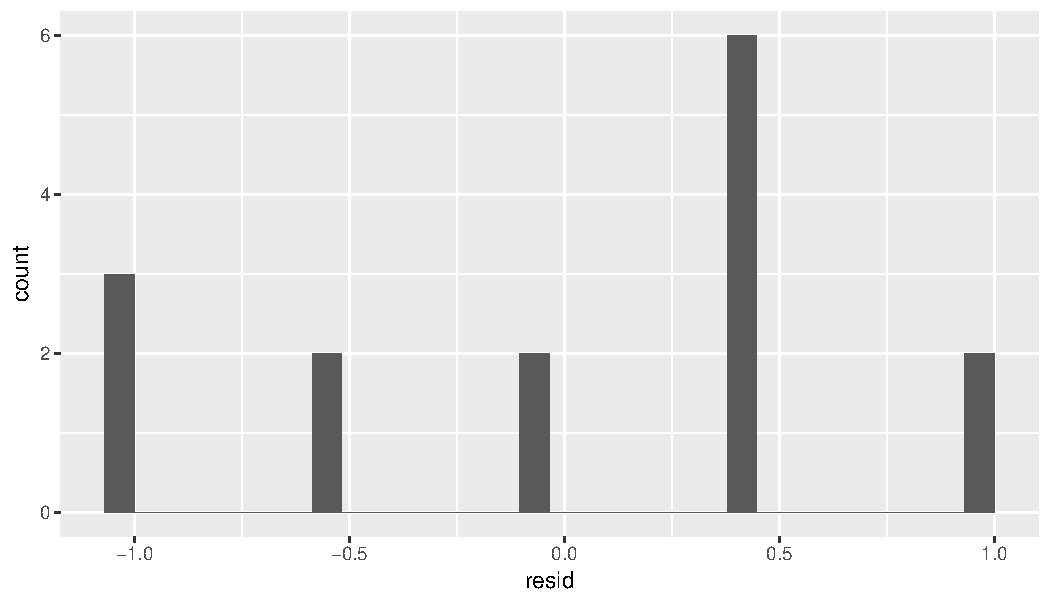
\includegraphics[width=\maxwidth]{figure/table1201-1} 

}



\end{knitrout}

Everytime we see a distribution of residuals that is either very skew, or has very few different values, we should consider a nonparametric analysis. Note that the shape of the distribution of the residuals is directly related to what scale values we choose for the ordinal categories. By changing the values we change the regression line, and that directly affects the relative sizes of the residuals. 

First, we will discuss a nonparametric alternative for two quantitative variables. We will start with Spearman's rho, or Spearmams rank-order correlation coefficient $r_s$. Next we will discuss an alternative to $r_s$, Kendall's T. After that we will discuss categorical variables, when comparing group differences.

\section{Spearman's rho}


Suppose we have 10 students and we ask their teachers to rate them. One teachers rates them on geography and the other teachers on history. We only ask to give rankings: indicate the brightest student with a 1 and the dullest student with a 10. Then we might have the following data set:



\begin{knitrout}
\definecolor{shadecolor}{rgb}{0.969, 0.969, 0.969}\color{fgcolor}
\begin{tabular}{r|r}
\hline
rank.geography & rank.history\\
\hline
5 & 4\\
\hline
4 & 5\\
\hline
6 & 7\\
\hline
7 & 8\\
\hline
8 & 6\\
\hline
9 & 9\\
\hline
10 & 10\\
\hline
2 & 3\\
\hline
1 & 1\\
\hline
3 & 2\\
\hline
\end{tabular}


\end{knitrout}

Now we acknowledge the ordinal nature of the data: we only have rankings: a person with rank 1 is brighter than a person with rank 2, but we do not how large the difference in brightness really is.  Now we want to establish whether there is a relationship between rankings on geography and the rankings on history: is it true that the higher the ranking on geography, the higher the ranking on history?


By eyeballing the data, we see that the brightest student in geography is also the brightest student in history (rank 1). We also see that the dullest student in history is the dullest student in geography (rank 10). Furthermore, we see relatively small differences between the rankings on the two subjects: high rankings on geography seem to go together with high rankings on history. Let;s look at these differences between rankings more closely by computing them:

\begin{knitrout}
\definecolor{shadecolor}{rgb}{0.969, 0.969, 0.969}\color{fgcolor}
\begin{tabular}{r|r|r}
\hline
rank.geography & rank.history & difference\\
\hline
5 & 4 & -1\\
\hline
4 & 5 & 1\\
\hline
6 & 7 & 1\\
\hline
7 & 8 & 1\\
\hline
8 & 6 & -2\\
\hline
9 & 9 & 0\\
\hline
10 & 10 & 0\\
\hline
2 & 3 & 1\\
\hline
1 & 1 & 0\\
\hline
3 & 2 & -1\\
\hline
\end{tabular}


\end{knitrout}

So theoretically the difference could be as large as 9, but here we see a biggest difference of -2. So the average difference is the sum of these differences, divided by 10, so we get 0. This is because we plus and minus values. If we would take the square of the differences, we would get positive values:

\begin{knitrout}
\definecolor{shadecolor}{rgb}{0.969, 0.969, 0.969}\color{fgcolor}
\begin{tabular}{r|r|r|r}
\hline
rank.geography & rank.history & difference & squared.difference\\
\hline
5 & 4 & -1 & 1\\
\hline
4 & 5 & 1 & 1\\
\hline
6 & 7 & 1 & 1\\
\hline
7 & 8 & 1 & 1\\
\hline
8 & 6 & -2 & 4\\
\hline
9 & 9 & 0 & 0\\
\hline
10 & 10 & 0 & 0\\
\hline
2 & 3 & 1 & 1\\
\hline
1 & 1 & 0 & 0\\
\hline
3 & 2 & -1 & 1\\
\hline
\end{tabular}


\end{knitrout}

Now we can compute the average squared difference, which is equal to 10/10 = 1. Generally, the smaller this value, the closer the rankings are together, and the more correlation there is between the two subjects. 

A clever mathematician like Spearman has shown that is even better to use a somewhat different measure for a correlation between ranks. He showed that it is wiser to compute the following statistic:

\begin{eqnarray}
r_s = 1 - \frac{6 \sum d^2 }{N^3-N}
\end{eqnarray}

because then you get a value between -1 and 1, just like a Pearson correlation. So in this case the sum of the squared difference is equal to 10, N is the number of students, so we get:


\begin{eqnarray}
r_s = 1 - \frac{6 \times 10  }{10^3-10} = 1 - 60 /990 = 0.94
\end{eqnarray}


 This is called the Spearman rank-order correlation coefficient $r_s$. It can be used for any two variables of which one is at most ordinal. The trick is to convert the scale values into ranks, and then apply the formula above. For instance, if we have the variable Grade with the following values (C, B, D, A, F), we convert them into rankings by saying the A is the highest value (1), B is the second highest value (2), C is the third highest value (3), D is the fourth highest value (4) and F is the fifth highest value (5). So tranformed into rankings we get (3, 2, 4, 1, 5). We can also let SPSS do the computations for us. Suppose we have two variables shoe size and aggression, we use the syntax:
 \begin{verbatim}
 NONPAR CORR 
   /VARIABLES=shoesize aggression 
  /PRINT=SPEARMAN .
 \end{verbatim}
  
In the output you will see a correlation matrix very similar the one for a Pearson correlation. Spearman's rho is equal to the $r_2$ mentioned above. You will also see whether the correlation is significantly different from 0, indicated by a $p$-value. If the $p$-value is very small, you may concluded that on the basis of these data, the correlation in the population is not equal to 0, ergo, in the population there is a relationship between shoe size and aggression.   
  

Below we discuss an alternative measure for a correlation for ordinal data, the Kendall rank-order correlation coefficient $T$. 


\section{Kendall rank-order correlation coefficient $T$}


If you want to know if there is a relationship between two variables, of which one is at most ordinal, you can either use Spearman's rho or Kendall's T. However, if you have three variables, and you want to know whether there is a relationship between A and B, over and above the effect of C, you can use a extension of Kendall's T. Note that this is very similar to multiple regression: a coefficient for variable $X_1$ in multiple regression with two predictors is the effect of $X_1$ on Y over and above the effect of $X_2$ on Y. The logic of Kendall's T is also based on rank orderings, but it involves a different computation. Let's look at the student data again with the teacher's rankings of the students on two subjects:

\begin{knitrout}
\definecolor{shadecolor}{rgb}{0.969, 0.969, 0.969}\color{fgcolor}
\begin{tabular}{r|r|r}
\hline
student & rank.geography & rank.history\\
\hline
1 & 5 & 4\\
\hline
2 & 4 & 5\\
\hline
3 & 6 & 7\\
\hline
4 & 7 & 8\\
\hline
5 & 8 & 6\\
\hline
6 & 9 & 9\\
\hline
7 & 10 & 10\\
\hline
8 & 2 & 3\\
\hline
9 & 1 & 1\\
\hline
10 & 3 & 2\\
\hline
\end{tabular}


\end{knitrout}


First we put the students in a new order, such that the brightest student in geography comes first, and the dullest last. This also changes the order in the variable history:
\begin{knitrout}
\definecolor{shadecolor}{rgb}{0.969, 0.969, 0.969}\color{fgcolor}
\begin{tabular}{r|r|r}
\hline
student & rank.geography & rank.history\\
\hline
9 & 1 & 1\\
\hline
8 & 2 & 3\\
\hline
10 & 3 & 2\\
\hline
2 & 4 & 5\\
\hline
1 & 5 & 4\\
\hline
3 & 6 & 7\\
\hline
4 & 7 & 8\\
\hline
5 & 8 & 6\\
\hline
6 & 9 & 9\\
\hline
7 & 10 & 10\\
\hline
\end{tabular}


\end{knitrout}

 From this we see that the history teacher agrees with the geography teacher that student 9 is brighter than student 8. They also agree that student 9 is brighter than sutduent 10. If we do this for all possible pairs of students, we can count the number of times that they agree and we can count the number of times that they disagree. The total number of possible pairs is equal to $10 \choose 2 $ $ = 90/2= 45$. So for example we might find for a data set on 10 students, that of all 45 pairs, the teachers agree 30 times, and disagree 15 times. Then we can compute Kendall's T as follows:
 
  \begin{eqnarray}
  T= \frac { agreements - disagreements }{total number of pairs} = \frac{30-15 }{45} = 0.33
  \end{eqnarray}

This T statistic varies between -1 and 1 and can therefore be seen as a nonparametric analog of a Pearson correlation. Here, the teachers more often agree than disagree, so the correlation is positive. A negative correlation means that the teachers more often disagree than agree on the relative brightness of their students. 

The computations are quite involving so we're very lucky that SPSS can do the tedious job for us, with the following syntax:


 \begin{verbatim}
 NONPAR CORR 
   /VARIABLES=shoesize aggression 
  /PRINT=KENDALL .
 \end{verbatim}


As said, the advantage of Kendall's T over Spearman's r is that Kendall's T can be extended to cover the case that you wish to establish the strength of the relationships of two variables A and B, over and above the relationship with C. %Unfortunately there is no easy way to do this in SPSS. See http://www-01.ibm.com/support/docview.wss?uid=swg21474822 for how to do this. More on this can be read in Siegel & Castellan (1988).

        
Now that we have discuss relationships between quantitative variables, let's have look at the case where we have categorical variables.


\section{Kruskall-Wallis test for group comparisons}


Suppose we have three groups of students that go on a field trip together: mathematicians, psychologists and engineers. Each can pick a rain coat, with five possible sizes: extra small, small, medium, large or extra large. We want to know if preferred size is different in the three populations, so that we can be better prepared in the future. Now we have information about size, but this knowledge is not quantitative: we do not know the difference in size between medium and large, only that large is larger than medium. We have ordinal data, so computing a mean is impossible here. Even we would assign values like 1= extra small, 2=small, 3= medium, etcetera, the mean would be rather meaningless as these values are arbitrary. So instead of focussing on means, we can focus on medians: the middle value. For instance, the median value for our sample of mathematicians could be medium, for our sample of psychologists small, and for our sample of engineers large. Our question might then be whether the median values in the populations are really different. 

This can be assessed using the Kruskall-Wallis test. Similar to Spearman's r and Kendall's T, the data are transformed into ranks. This is done for all data at once, so for all students toghether.

For example, if we had the following data:
\\
 \\
 \begin{tabular}{lll}
 student & group & size \\ \hline
 001 & math & xs \\
 002 & math & xl \\
 003 & psych & m \\
 004 & psych & s \\
 005 & engineer & l \\
 \dots & \dots & \dots \\
 \end{tabular}
\\
\\
We would transform it into ranks, from smallest to largest, like this:
\\
 \\
 \begin{tabular}{lllr}
 student & group & size & rank\\ \hline
 001 & math & xs & 1\\
 002 & math & xl & 5\\
 003 & psych & m & 3\\
 004 & psych & s & 2\\
 005 & engineer & l & 4 \\
 \dots & \dots & \dots & \dots \\
 \end{tabular}
\\
\\
Next, we could compute the average rank per group. The group with the smallest sizes would have the lowest average rank, etcetera. Under the null-hypothesis, if the distribution of size was the same in all three groups, the average ranks would be about the same. If they are very different, this is an indication that size is not distributed equally among the three groups. In order to have a proper statistical test, a rather complex formula is used to compute the so-called KW statistics. We know the distribution of this KW statistic under the null-hypothesis, so we know what extreme values are, and consequently can compute p-values. This tedious computation is also done by SPSS using the following syntax. 

\begin{verbatim}
NPTESTS 
  /INDEPENDENT TEST (size) GROUP (group) KRUSKAL_WALLIS(COMPARE=NONE).
\end{verbatim}


The output gives you a significance level ($p$-value) of the test that size is distributed equally among psychology students, engineering students and mathematics students. If it is a very low number, you may conclude that in the population, students in psychology, mathematics in engineering have different preferences regarding the size of their rain coat on field trips. 


 % nonparametric alternatives linear models


\chapter{Linear mixed modelling: introduction}


\section{Fixed effects and random effects}
In the simplest form of linear modelling, we have one dependent continuous variable, one intercept and one or more independent variables. Let's look at a simple regression equation where dependent variable $y$ is predicted by an intercept $b_0$ and a linear effect of independent variable $x_1$ with regression slope parameter $b_1$, and an error term $e$, where we assume that the error term $e$ comes from a normal distribution. 


\begin{eqnarray}
y = b_0 + b_1 x_1 + e \\
e \sim N(0, \sigma^2)
\end{eqnarray}

Using this model, we know that for a person with a value of 5 for $x_1$, we expect $y$ to be equal to $b_0 + b_1 \times 5$. As another example, if $y$ is someone's IQ score, $x_1$ is someone's brain size in cubic milliliters, $b_0$ is equal to 70, and $b_1$ is equal to 0.1, we expect on the basis of this model that a person with a brain size of 1500 cubic millimeters has an IQ score of $70 + 0.01 \times 1500$, which equals 85.
\\
\\
Now, for any model the predicted values usually are not the same as the observed values. If the model predicts on the basis of my brain size that my IQ is 140, my true IQ might be in fact 130. This discrepancy is termed the residual: the observed $y$, minus the predicted $y$, or $\hat{y}$, so in this case the residual is $y - \hat{y}=130-140= -10$.
\\
\\
Here we have the model for the relationship between IQ and brain size.

\begin{eqnarray}
IQ = 70 + 0.1 \times Brainsize + e \\
e \sim N(0, \sigma^2)
\end{eqnarray}

Note that in this model, the values of 70 and 0.1 are \textit{fixed}, that is, we use the same intercept and the same slope for everyone. You use these values for any person, for Henry, Jake, Lizz, and Margaret. We therefore call these effects of intercept and slope \textit{fixed effects}, as they are all the same for all research units. In contrast, we call the $e$ term, the random error term or the residual in the regression, a \textit{random effect}. This is because the error term is \textit{different for every research unit}. We don't know the specific values of these random errors or residuals for every person, but nevertheless, we assume that they come from a distribution, in this case a normal distribution with mean 0 and an unknown variance. This unknown variance is given the symbol $\sigma^2$ 

Here are a few more examples. 

\begin{enumerate}
\item Suppose we study a number of schools, and for every school we use a simple linear regression equation to predict the number of students (dependent variable) on the basis of the number of teachers (independent variable). For every research unit (in this case: school), the intercept and the regression slope are the same (fixed effects), but the residuals are different (random effect). 

\item Suppose we study a number of students, and for every student we use a simple linear regression equation to predict the math test score on the basis of the number of hours of study the student puts in. Here, the research unit is student, and for every student, the  intercept and the regression slope are the same (fixed effects), but the residuals are different (random effect).

\item Suppose we study reaction times, and for every measure of reaction time -- a trial -- we use a simple linear regression equation to predict reaction time in milliseconds on the basis of the characteristics of the stimulus. Here, the research unit is trial, and for every trial, the intercept and the regression slope are the same (fixed effects), but the residuals are different (random effect).
\end{enumerate}

Now, what happens when we have a lot of data on students, but the students come from different schools? Suppose we want to predict average grade for every student, on the basis of the number of hours of study the student puts in. We again could use a simple linear regression equation. 

\begin{eqnarray}
y = b_0 + b_1 hourswork + e \\
e \sim N(0, \sigma^2)
\end{eqnarray}



That would be fine if all schools would be all very similar. But suppose that some schools have a lot of high scoring students, and some schools have a lot of low scoring students? Then school itself would also be a very important predictor, apart from the number of hours of study. One thing we could therefore do is to include school as a categorical predictor. We would then have to code this school variable into a number of dummy variables. The first dummy variable called $school1$ would indicate whether students are in the first school (school1=1) or not (school1=0). The second dummy variable $school2$ would indicate whether students are in the second school (school2=1) or not (school2=0), etcetera. You can then add these dummy variables to the regression equation like this:

\begin{eqnarray}
y = b_0 + b_1 hourswork + b_2 school1 + b_3 school2 + b_4 school3 + ... + e  \nonumber\\
e \sim N(0, \sigma^2)  \nonumber
\end{eqnarray}

In the output we would find a large number of effects, one for each dummy variable. For example, if the students came from 100 different schools, I would get 99 fixed effects for the 99 dummy variables. However, one could wonder whether this is very useful. As stated earlier, fixed effects are called fixed because they are the same for every unit of research, in this case every student. But working with 99 dummy variables, where students mostly score 0, this seems very much over the top. In fact, we're not even interested in these 99 effects. We're interested in the relationship between test score and hours of work, meanwhile taking into account that there are test score differences across schools. The dummy variables are only there to account for differences across schools; the prediction for one school is a little bit higher or lower than for another school, depending on how well students generally perform in each school. 
\\
\\
We could therefore try an alternative model, where we treat the school effect as $random$: we assume that every school has a different average test score, and that these averages are normally distributed. We call these average test score deviations \textit{school effects}:

\begin{eqnarray}
y = b_0 + b_1 hourswork + schooleffect + e \\
schooleffect \sim N(0, \sigma_s^2)\\
e \sim N(0, \sigma_e^2)
\end{eqnarray}

So in this equation, the intercept is fixed, that is, the intercept is the same for all observed test scores. The regression coefficient $b_1$ for the effect of hours of work is also fixed. But the schooleffect is random, since it is different for every school. The residual $e$ is also random, being different for every student. It could also be written like this:

\begin{eqnarray}
y = (b_0  + schooleffect) + b_1 hourswork + e \\
schooleffect \sim N(0, \sigma_s^2)\\
e \sim N(0, \sigma_e^2)
\end{eqnarray}


This representation emphasizes that for every school, the intercept is a little bit different: for school A the intercept might be $b_0 + 2$, and for school R the intercept might be $b_0 - 3$.

So, this equation states that every observed test score is 1) partly influenced by an intercept that is random, with a certain average $b_0$ and variance $\sigma_s^2$, that is dependent on which school students are in, 2) partly influenced by the number of hours of work, an effect that is the same no matter what school a student is in (fixed), and 3) partly influenced by unknown factors, indicated by a random residual $e$ coming from a normal distribution with variance $\sigma^2_e$.

To put it more formally: test score $y_{ij}$, that is, the test score from student $j$ in school $i$, is the sum of an effect of the school $b_0 + schooleffect_i$ (the average test score in school $i$), plus an effect of hours of work,  $b_1 \times hourswork$, and an unknown residual $e_{ij}$ (a specific residual for the test score for studuent $j$ in school $i$).

\begin{eqnarray}
y_{ij} = b_0 + schooleffect_i + b_1 hourswork + e_{ij} \\
schooleffect_i \sim N(0, \sigma_s^2)\\
e_{ij} \sim N(0, \sigma_e^2)
\end{eqnarray}

So in addition to the assumption of residuals that have a normal distribution with mean 0 and variance $\sigma_s^2$, we also have an assumption that the school averages are normally distributed, in this case with mean $b_0$ and variance $\sigma_s^2$.
\\
\\
Let's go back to the example of reaction times. Suppose in an experiment we measure reaction time in a large number of trials. We want to know whether the size of the stimulus (large/small) has an effect on reaction time. Let's also suppose that we carry out this experiment with 20 participants, where every participant is measured during 100 trials: 50 large stimuli and 50 small stimuli in random order. Now probably, some participants show generally very fast responses, and some participants show generally very slow responses. In other words, the average reaction time for the 100 trials may vary from participant to participant. This means that we can use participant as an important predictor of reaction times. To take this into account we can use the following equation:


\begin{eqnarray}
y_{ij} = b_0 + speed_i + b_1 size + e_{ij} \\
speed_i \sim N(0, \sigma_s^2)\\
e_{ij} \sim N(0, \sigma_e^2),
\end{eqnarray}

where $y_{ij}$, is the reaction time $j$ from participant $i$, $(b_0 + speed_i)$ is a random effect representing the average speed for each participant $i$ (where $b_0$ is the overall average across all participants), $b_1$ is the fixed effect of the size of the stimulus, and unknown residual $e_{ij}$ is a specific residual for the reaction time for trial $j$ of participant $i$.
\\
\\
The reason for introducing random effects is that when your observed data are clustered, for instance student scores clustered within schools, or trial response times are clustered within participants, you violate the assumption of independence: two reaction times from the same person are more similar than two reaction times from different persons. Two test scores from students from the same school may be more similar than two scores from students in different schools. When this is the case, when data are clustered, it is very important to take this into account. When the assumption of independence is violated, you are making wrong inference if you only use a simple linear model. With clustered data, it is therefore necessary to work with an extension of the linear model, the so-called linear mixed model. The above models for test scores across different schools and reaction times across different participants, are examples of \textit{linear mixed models}. The term \textit{mixed} comes from the fact that the models contain a mix of both fixed and random effects. 
\\
\\
If you have clustered data, you should take this clustering into account, either by using the grouping variable as a qualitative predictor (using a number of dummy variables) or by using a linear mixed model. As a rule of thumb: if you have fewer than 10 groups, consider dummy variables; if you have 10 or more groups, consider a linear mixed model. Use a linear mixed model if the assumption of normally distributed group differences is tenable. Use dummy variables if you are actually interested in the size of group differences.
\\
\\
Below, we will start with a very simple example of linear mixed model, one that we use for a simple pre-post intervention design.



\section{Pre-post intervention design}


Imagine a study where we hope to show that aspirin helps reduce headache. For 100 patients we ask to rate the severity of their headache before they use aspirin (on a scale from 1 - 100), and to rate the severity again 3 hours after taking 500 mg of aspirin. These patients were randomly selected among people who read the NY Times and suffer from regular headaches. So here we have clustered data: we have 100 patients, and for each patient we have two scores, one before (pre) and one after (post) the intervention of taking aspirin. Of course headaches differ from person to person, so we might have to take into account that some patients have a higher average level of headache than other patients. Now, the data could be represented in different ways, but suppose we have the following data matrix (showing only the first 5 patients):
 \\
 \\
 \begin{tabular}{lrr}
 patient & pre & post \\ \hline
 001 & 55 & 45 \\
 002 & 63 & 50 \\
 003 & 66 & 56 \\
 004 & 50 & 37 \\
 005 & 63 & 50 \\
 \dots & \dots & \dots \\
 \end{tabular}
\\
\\
What we observe here is that the severity seems generally lower after the intervention than before the intervention. But you may also notice that the severity of the headache also varies across patients: some have generally high scores (for instance patient 003), and some have generally low scores (for example patient 001). Therefore, the headache scores seem to be clustered, violating the assumption of independence. We can quantify this clustering by computing a correlation between the pre-intervention scores and the post-intervention scores. Here it appears that there is a strong positive correlation, indicating that the higher the pain score before the intervention, the higher the pain score after the intervention. 
\\
\\

There is an alternative way of representing the same data. Let's look at the same data in a new format:
\begin{knitrout}
\definecolor{shadecolor}{rgb}{0.969, 0.969, 0.969}\color{fgcolor}
\begin{tabular}{r|r|r}
\hline
patient & measure & headache\\
\hline
1 & 1 & 55\\
\hline
1 & 2 & 45\\
\hline
2 & 1 & 63\\
\hline
2 & 2 & 50\\
\hline
3 & 1 & 66\\
\hline
3 & 2 & 56\\
\hline
4 & 1 & 50\\
\hline
4 & 2 & 37\\
\hline
5 & 1 & 63\\
\hline
5 & 2 & 50\\
\hline
\end{tabular}


\end{knitrout}
%  \\
%  \\
%  \begin{tabular}{lrr}
%  patient & intervention & severity \\ \hline
%  001 & pre & 80 \\
%  001 & post & 65 \\
%  002 & pre & 34 \\
%  002 & post & 25 \\
%  003 & pre & 23 \\
%  003 & pre & 15 \\
%  004 & post & 90 \\
%  004 & pre & 70 \\
%  005 & post & 23 \\
%  005 & pre & 13 \\
%  \dots & \dots & \dots \\
%  \end{tabular}
% \\
% \\
Here we acknowledge that there is really only one dependent measure: headache severity. The other two variables indicate that this variable varies across both patients and time point (pre intervention and post intervention). Here we might consider applying a simple linear regression model, using severity as the dependent variable and \textbf{measure} (1st or 2nd) as a qualitative predictor (using a dummy variable). However, since we know that there is a correlation between the pre and post severity measures, we know that measures systematically vary across patients: some score high on average and some score low on average. Therefore we have to run a linear \textit{mixed} model, including not only the fixed effect of \textbf{measure} but also a random effect for each patient. Since we are really interested in the effect of the intervention, that is, we want to know how large the effect of aspirin is, we use a fixed effect for the time effect (the variable \textbf{measure}). For the patient effect, because there are so many patients (100) and we're really not interested in all of these individual differences, we use a random effect. This means that we only assume there is a normal distribution for all of the patient differences. So we get the following equation:


\begin{eqnarray}
y_{ij} = b_0 + patient_i + b_1 measure + e_{ij} \\
patient_i \sim N(0, \sigma_p^2)\\
e_{ij} \sim N(0, \sigma_e^2)
\end{eqnarray}

$y_{ij}$ is the $j$th headache severity score (first or second) for patient $i$, $(b_0 + patient_i)$ is the average headache for patient $i$, \textit{measure} is a dummy variable for which measure (first or second), and $b_1$ is the effect of the intervention (by how much the severity changes from pre to post). We assume that the average pain level for each patient shows a normal distribution with average $b_0$ and variance $\sigma^2_p$. And of course we assume that the residuals show a normal distribution.
\\
\\
This analysis can be done with the following SPSS syntax, treating time as a qualitative variable (using BY) for which SPSS will create a dummy variable automatically. 


\begin{verbatim}
MIXED headache  BY measure
  /FIXED=measure
  /PRINT=DESCRIPTIVES  SOLUTION
  /RANDOM=intercept | SUBJECT(patient) COVTYPE(VC).
\end{verbatim}


\begin{figure}[h]
    \begin{center}
       \includegraphics[scale=0.8, trim={0cm 20cm 0cm 0cm} ]{/Users/stephanievandenberg/Dropbox/Statistiek_Onderwijs/Data" "Analysis/spss" "examples" "linear" "mixed" "model/prepost/prepost.pdf}
    \end{center}
\end{figure}

The most interesting output is given here. We're mostly interested in the fixed effect of the intervention: does aspirin reduce headache? After an F-test, we see the linear model coefficients, with an intercept of around 49 and a positive effect of the intervention dummy variable, around $+10$. We see that the dummy variable was coded 0 for the second measure and 1 for first meausure. So, for our dependent variable headache, we see that the expected headache severity for the observations with a 0 for the dummy variable (that is, measure 2, which is \textit{after} taking aspirin), is equal to $49 + (10) \times 0 = 49$. Similarly, we see that the expected headache severity for the observations with a 1 for the dummy variable (that is, \textit{before} taking aspirin), is equal to $49 + (10) \times 1 = 49 + 10 = 59$. So, average pain severity is 10 points higher before the intervention than after the intervention. Whether this difference is significant is indicated by a $t$-test. We see here that the average headache severity after taking an aspirin is significantly different from the average headache severity before taking an aspirin, $t(99) = 25.46, p < 0.01$. The degrees of freedom are taken from the Test of Fixed Effects table with the $F$-statistics. Alternatively we can write 

\begin{quote}
{The average headache severity after taking an aspirin is significantly different from the average headache severity before taking an aspirin, $F(1,99) = 648.28, p < 0.01$}\end{quote}


We might therefore carefully conclude that aspirin reduces headache in the population of NY Times readers with headache problems, where the reduction is around 10 points on a 1...100 scale (95\% CI: 9.55 -- 11.17). 
\\
\\
Now, this looks like reporting the output of a regular linear model, but of course it isn't. We also have some extra output, about the random effect of patient. We assumed that the individual differences in headache severity in the 100 patients came from a normal distribution. How large are these individual differences actually? This can be gleaned from the Covariance Parameters part of the SPSS output. We there see two random effects: the one for the residuals and one for the patients. The intercept seems to vary with a variance of 27, which is equivalent to a standard deviation of $\sqrt{27}$ which is around 5.2. What does that mean exactly? Well let's look at the equation again and fill in the numbers:

\begin{eqnarray}
y_{ij} = b_0 + patient_i + b_1 measure + e_{ij} \\
y_{ij} = 49 + patient_i + 10 measure + e_{ij} \\
patient_i \sim N(0, 27)\\
e_{ij} \sim N(0, 8)
\end{eqnarray}

Since measure is coded 0 for the headache level after the intervention, we conclude that the average pain level after taking aspirin is 49. However, not everybody's pain level after taking aspirin is 49: people show variance. The pain level after aspirin varies with a variance of 27, which is equavalent to a standard deviation of arond 5.2. Figure below shows how much this variance actually is. It depicts a normal distribution with mean 49 and a standard deviation of 5.2.


\begin{knitrout}
\definecolor{shadecolor}{rgb}{0.969, 0.969, 0.969}\color{fgcolor}

{\centering 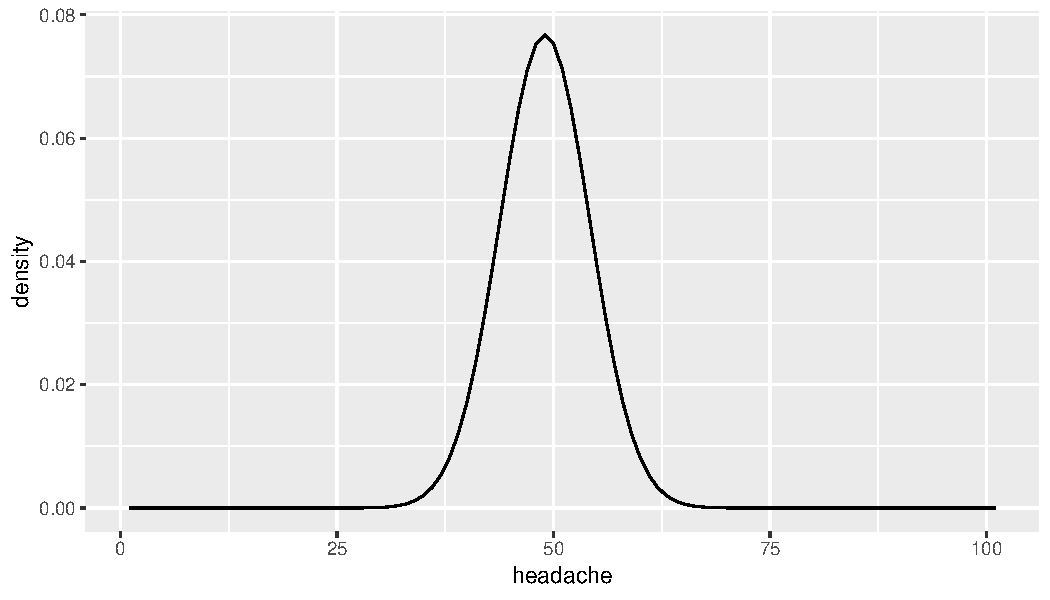
\includegraphics[width=\maxwidth]{figure/resultsprepost1-1} 

}



\end{knitrout}

So \textit{after} taking aspirin, most patients show headache levels between 30 and 60. More specificially, if we would take the middle 95\% by using plus or minus twice the standard deviation, we can estimate that 95\% of the patients shows levels between $49 - 2 \times 5.2 = 38.6$ and $49 + 2 \times 5.2 = 59.4$
\\
\\
Now let's look at the levels \textit{before} taking aspirin. The average headache leves is equal to $49 + 10 = 59$. So 95\% of the patients shows headache levels between $59 - 2 \times 5.2 = 48.6$ and $59 + 2 \times 5.2 = 49.4$ before taking aspirin. 
\\
\\
Together these results can be graphically explained in the plot below:
\begin{knitrout}
\definecolor{shadecolor}{rgb}{0.969, 0.969, 0.969}\color{fgcolor}

{\centering 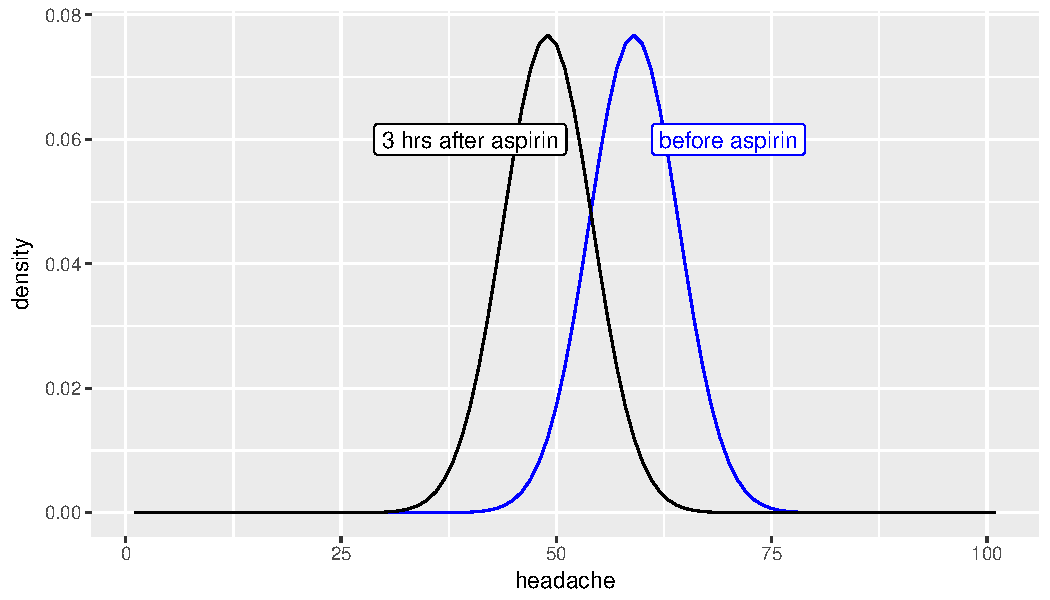
\includegraphics[width=\maxwidth]{figure/resultsanalysisprepost2-1} 

}



\end{knitrout}


In this plot you see there is variability in headache levels before taking aspirin, and there is variation in headache levels after taking aspirin. We also see that these distributions have the same spread (variance): in the model we assume that the variability in headache before aspirin is equal to the variability after aspirin. The distributions are equal, except for a horizontal shift: the distribution for heachache after aspirin is the same as the distribution before apsirin, except for a shift to the left of about 10 points. This is of course the effect of aspirin in the model, the $b_1$ parameter in our model above. 
\\
\\
The fact that the two distributions before and after aspirin show the same spread (variance) was an inherent assumption in our model: we only have one random effect for patient in our output. If the assumption of equal variance (homoscedasticity) is not tenable, then one should consider other linear mixed models. But this is beyond the scope of this chapter. The assumption can be checked by plotting the residuals, using differnt colours for residuals from before taking aspirin and for residuals from after taking aspirin. 



\subsection{Exercises}

Suppose an intervention study looked at the effect of therapy on depression levels. A random sample of patients were measured before and after the therapy. Given the following equation, based on output of the statistical software package R. The dummy variable \textit{measure} was coded 0 for before therapy and 1 for after therapy.




\begin{figure}[h]
    \begin{center}
       \includegraphics[scale=0.8, trim={0cm 20cm 0cm 0cm}]{/Users/stephanievandenberg/Dropbox/Statistiek_Onderwijs/Data" "Analysis/spss" "examples" "linear" "mixed" "model/prepost/prepostdepression.pdf}
    \end{center}
\end{figure}


Look at the output below. You see information about random effects and you see information about fixed effects. 

\begin{itemize}
\item 1. What is the intercept of the model?\\
\item 2. What is the slope coefficent for the measure variable?\\
\item 3. What is the variance of the residuals? What is the standard deviation?\\
\item 4. What is the variance of the individual differences among patients? What is the standard deviation?\\
\item 5. Fill in the values in the linear mixed model below:

\begin{eqnarray}
depression_{ij} = \dots + patient_i + \dots \times measure + e_{ij} \\
patient_i \sim N(0, \sigma_p^2 = \dots)\\
e_{ij} \sim N(0, \sigma_e^2 = \dots)
\end{eqnarray}


\item 6. what can you say about the average depression level before therapy? \\
\item 7. what can you say about the average depression level after therapy?\\
\item 8. How much variance in depression level before therapy does this model predict? What is the standard deviation? \\
\item 9. Between what values do depression levels before therapy in the middle 95\% of patients show?\\
\item 10. How much variance in depression level after therapy does this model predict? What is the standard deviation? \\
\item 11. Between what values do depression levels after therapy in the middle 95\% of patients show?\\
\item 12. Does therapy help to alleviate depression in patients? You may use an approximation to construct a confidence interval.

\item 13. A researcher has two groups of patients: one group receives medicine and one group receives therapy. The null-hypothesis is that depression levels after medicine are as high as depression levels after therapy. Do we analyse these data with an ordinary linear model, or with a linear mixed model? Explain your answer.

\item 14. A researcher studies one group of students: they first get lectures from teacher A and then they get lectures from teacher B. The null-hypothesis is that the average teacher evaluation for teacher A is the same as the average teacher evaluation for teacher B. Do we analyse these data with an ordinary linear model, or with a linear mixed model? Explain your answer. 


\item 15. For a study to the effect of light on mood, we have data on 100 teachers They were asked to rate their mood on a cloudy day and asked to rate their mood on a sunny day. We have the variable \textbf{mood}, the dummy variable \textbf{sunny} and we want to include a random effect for \textbf{teacher} From the three syntaxes below, choose the one that is most suitable for your analysis and fill in the blanks.


\begin{verbatim}
MIXED ...  WITH ...
  /FIXED=...
  /PRINT=DESCRIPTIVES  SOLUTION
  /RANDOM=intercept | SUBJECT(...) COVTYPE(VC).
\end{verbatim}


\begin{verbatim}
UNIANOVA ... WITH ... 
/ design = ...
/ print = parameter.
\end{verbatim}


\begin{verbatim}
UNIANOVA ... BY ... 
/ design = ...
/ print = parameter.
\end{verbatim}


\item 16. A researcher wants to know whether students in green classrooms (colour = 1) perform better than students in yellow classrooms (colour = 2). The following data were collected (showing only a part):

\begin{knitrout}
\definecolor{shadecolor}{rgb}{0.969, 0.969, 0.969}\color{fgcolor}
\begin{tabular}{r|r|r}
\hline
student & colour & performance\\
\hline
1 & 1 & 6.79\\
\hline
2 & 2 & 8.28\\
\hline
3 & 1 & 9.08\\
\hline
4 & 2 & 5.65\\
\hline
5 & 1 & 8.43\\
\hline
6 & 2 & 8.51\\
\hline
7 & 1 & 7.43\\
\hline
8 & 2 & 7.45\\
\hline
9 & 1 & 7.44\\
\hline
10 & 2 & 7.11\\
\hline
\end{tabular}


\end{knitrout}

Would you use an ordinary linear model or a linear mixed model to analyze these data? Explain your answer.

\item 17. A researcher wants to know whether students in dark classrooms (brightness = 0) perform better than students in bright classrooms (brightness = 1). The following data were collected (showing only a part):


\begin{knitrout}
\definecolor{shadecolor}{rgb}{0.969, 0.969, 0.969}\color{fgcolor}
\begin{tabular}{r|r|r}
\hline
student & brightness & performance\\
\hline
1 & 0 & 8.66\\
\hline
1 & 1 & 5.95\\
\hline
2 & 0 & 6.50\\
\hline
2 & 1 & 9.47\\
\hline
3 & 0 & 9.46\\
\hline
3 & 1 & 8.14\\
\hline
4 & 0 & 8.21\\
\hline
4 & 1 & 4.96\\
\hline
5 & 0 & 7.51\\
\hline
5 & 1 & 6.91\\
\hline
\end{tabular}


\end{knitrout}

Would you use an ordinary linear model or a linear mixed model to analyze these data? Explain your answer.



\item 18.
A landscaper believes that people get more creative once the environment becomes greener. She measures creativity before and after the introduction of new trees around the office building in a random sample of employees. Because creativity can also be influenced by the weather she also uses a dummy variable \textbf{sunny} to correct for these effects. Whether creativity is meassured before or after the introduction of the trees is indicated by the variable \textbf{green} that is coded green=1 for after the introduction and green=0 for before the introduction. The model that she therefore runs in SPSS is the following:

\begin{verbatim}
MIXED creativity  WITH green sunny
  /FIXED= green sunny
  /PRINT=DESCRIPTIVES  SOLUTION
  /RANDOM=intercept | SUBJECT(employee) COVTYPE(VC).
\end{verbatim}

We get the following output: 

\begin{figure}[h]
    \begin{center}
       \includegraphics[scale=0.8, trim={0cm 20cm 0cm 0cm}]{/Users/stephanievandenberg/Dropbox/Statistiek_Onderwijs/Data" "Analysis/spss" "examples" "linear" "mixed" "model/prepost/prepostcreativity.pdf}
    \end{center}
\end{figure}

Write a short paragraph describing these results and the conclusions in APA format.


\end{itemize}


\subsubsection{Answers:}

\begin{itemize}

\item Ad1: 10.57 \\
\item Ad2: -2.28 \\
\item Ad3: 8.31,2.88 \\
\item Ad4: 1.79,1.34 \\

\item Ad5:
\begin{eqnarray}
depression_{ij} = 10.57 + patient_i + (-2.28) \times measure + e_{ij} \\
patient_i \sim N(0, \sigma_p^2 = 1.79)\\
e_{ij} \sim N(0, \sigma_e^2 = 8.31)
\end{eqnarray}




\item Ad 6: 10.57\\
\item Ad 7: 10.57 + -2.28  = 8.29\\
% Ad 8: SD = 1.34, variance is 1.34^2= 1.80$. \\
\item Ad 8: 1.79, 1.34 \\

\item Ad 9: $10.57 \pm 2 \times 1.34 = {7.89, 13.25}$\\

\item Ad 10: 1.79, 1.34 \\

\item Ad 11: $(10.57 -2.28)  \pm  2 \times 1.34 = {5.61, 10.79 }   $\\

\item Ad 12: For the effect of therapy (the measure variable), we see a $b$-value of -2.28 with a standard error of 0.407773, so if we use the +/-2 rule to compute a 95\% confidence interval, we get $[ -2.28 - 2\times 0.41 , -2.28 + 2\times 0.41]  = [ -3.1 ,  -1.46]$. The 95\% interval does NOT contain the value 0 so we can reject the null-hypothesis that the effect of therapy is zero. Therefore, we conclude that therapy has an influence on depression. In this case we saw a decrease in depression levels after therapy.

\item Ad 13: Two groups of patients are studied, and for each patient we have only one measure. Because we only have one measure for each unit of observation we conduct an ordinary linear model.

\item Ad 14: One group of students is studied, and for each student we have two evaluations: one for teacher A and one for teacher B. Because we have more than one measure for each unit of observation, we have to use a linear mixed model. 

\item Ad15: 

\begin{verbatim}
MIXED mood  WITH sunny
  /FIXED=sunny
  /PRINT=DESCRIPTIVES  SOLUTION
  /RANDOM=intercept | SUBJECT(teacher) COVTYPE(VC).
\end{verbatim}

\item Ad16: it seems as if each student was only measured once, there is no clustering, so we can use an ordinary linear model.

\item Ad17: it seems as if each student was measured twice, in both dark and bright conditions, so we use a linear mixed model to account for clustering.

\item Ad18: 
\begin{quotation}

A linear mixed model was run to test the effect of green surroundings on creativity. The analysis was corrected for the effects of weather (sunny or not sunny) and random effects for employees. The results showed a significant but negative effect of the introduction of trees on creativity: creativity was on average 4.5 points lower after the introduction, $t(98)=-10.47, p < 0.001$. This effect was present over and above the effect of the weather which by itself had also an effect, where creativity was 1.28 points lower on sunny days than on not cloudy days, $t(98)=-2.32, p=0.02$. The variance not explained by weather and greenness was largely explained by individual differences in creativity among employees, with an intraclass correlation of $\frac{23.7}{23.7+9.2}= 0.72$. We conclude that the introduction of trees has a negative influence on creativity in the employees that worked in the building studied in this research. 

\end{quotation}

\end{itemize}



\section{Pre-mid-post intervention design}


In many intervention studies, one has more than two measurement moments. For instance, you'd like to know if there is not only a short term effect of aspirin, but also a long-term effect. Suppose that the study mentioned in the previous section on headache among NY Times readers was extended by asking patients not only to rate their headache before aspirin and 3 hours after intake, but also 24 hours after intake. In this case our data could look like this:

\begin{knitrout}
\definecolor{shadecolor}{rgb}{0.969, 0.969, 0.969}\color{fgcolor}
\begin{tabular}{r|r|r|r}
\hline
patient & measure1 & measure2 & measure3\\
\hline
1 & 52 & 45 & 47\\
\hline
2 & 59 & 50 & 55\\
\hline
3 & 65 & 56 & 58\\
\hline
4 & 51 & 37 & 42\\
\hline
5 & 62 & 50 & 55\\
\hline
6 & 61 & 53 & 57\\
\hline
7 & 56 & 44 & 55\\
\hline
8 & 62 & 48 & 53\\
\hline
9 & 56 & 48 & 49\\
\hline
10 & 58 & 45 & 44\\
\hline
\end{tabular}


\end{knitrout}

So for each patient we have three measures: pre, post1 and post2. To see if there is some significant clustering, it is no longer possible to study this by computing a single correlation. We could however compute 3 different correlations: pre-post1, pre-post2, and post1-post2, but this is rather tedious, and moreover does not give us a single measure of the extent of clustering of the data. But there is an alternative: one could compute not a Pearson correlation, but an \textit{intraclass correlation} (ICC). To do this, we need to bring the data again into a regression type format, like this (we call this \textit{long format}, as opposed to \textit{wide format}):

\begin{knitrout}
\definecolor{shadecolor}{rgb}{0.969, 0.969, 0.969}\color{fgcolor}
\begin{tabular}{r|r|r}
\hline
patient & measure & headache\\
\hline
1 & 1 & 52\\
\hline
1 & 2 & 45\\
\hline
1 & 3 & 47\\
\hline
2 & 1 & 59\\
\hline
2 & 2 & 50\\
\hline
2 & 3 & 55\\
\hline
3 & 1 & 65\\
\hline
3 & 2 & 56\\
\hline
3 & 3 & 58\\
\hline
4 & 1 & 51\\
\hline
\end{tabular}


\end{knitrout}

We can perform an analysis using a MIXED analysis in SPSS:

\begin{verbatim}

MIXED headache BY measure
  /FIXED=measure
  /PRINT=DESCRIPTIVES  SOLUTION
  /RANDOM=intercept | SUBJECT(patient) COVTYPE(VC).
\end{verbatim}

The output is given below:

\begin{figure}[h]
    \begin{center}
       \includegraphics[scale=0.8, trim={0cm 20cm 0cm 0cm} ]{/Users/stephanievandenberg/Dropbox/Statistiek_Onderwijs/Data" "Analysis/spss" "examples" "linear" "mixed" "model/premidpost/premidpostaspirin.pdf}
    \end{center}
\end{figure}


In the output we see the fixed effects of two automatically created dummy variables \textbf{measure=1} and \textbf{measure=2}, and the intercept. We also see the variances of the random effects: the variance of the residuals and the variance of the random effects for each patient.

From this output, we can plug in the values into the equation:


\begin{eqnarray}
headache_{ij} = 51 + patient_i +7.5 \times measure1 - 2.4 \times measure2 + e_{ij} \nonumber\\
patient_i \sim N(0, 28.3)\nonumber\\
e_{ij} \sim N(0, 8.5)\nonumber
\end{eqnarray}

Based on this equation, the expected headache severity score in the population 24 hours after aspirin intake is 51 (the third measure is the reference group). Dummy variable \textbf{measure=1} is coded 1 for the measurements before taking aspirin. Therefore, the expected headache score before aspirin intake is equal to $51+7.5 = 58.5$. Dummy variable \textbf{measure=2} was coded 1 for the measurements 3 hours after aspirin intake. Therefore, the expected headache score 3 hours after aspirin intake is equal to $51 - 2.4 = 48.6$. In sum, in this sample we see that the average headache level decreases directly after aspirin intake from 58.5 to 48.6, but then increases again to 51. 
\\
\\
There was quite some variation in individual headache levels: the variance is equal to 28.3, so the standard deviation (its square root) is equal to about 5.3. Therefore, if we look at roughly 95\% of the sample, we see that prior to taking aspirin, the scores vary between $58.5 -2\times 5.3 = 47.9$ and $58.5 + 2 \times 5.3 = 69.1$. For the short-term effect of aspirin after 3 hours, we see that roughly 95\% of the scores lie between $48.6 -2\times 5.3 = 38.0$ and $48.6 + 2 \times 5.3 = 59.2$. The normal distributions, predicted by this model, are depicted in the figure below:


\begin{knitrout}
\definecolor{shadecolor}{rgb}{0.969, 0.969, 0.969}\color{fgcolor}

{\centering 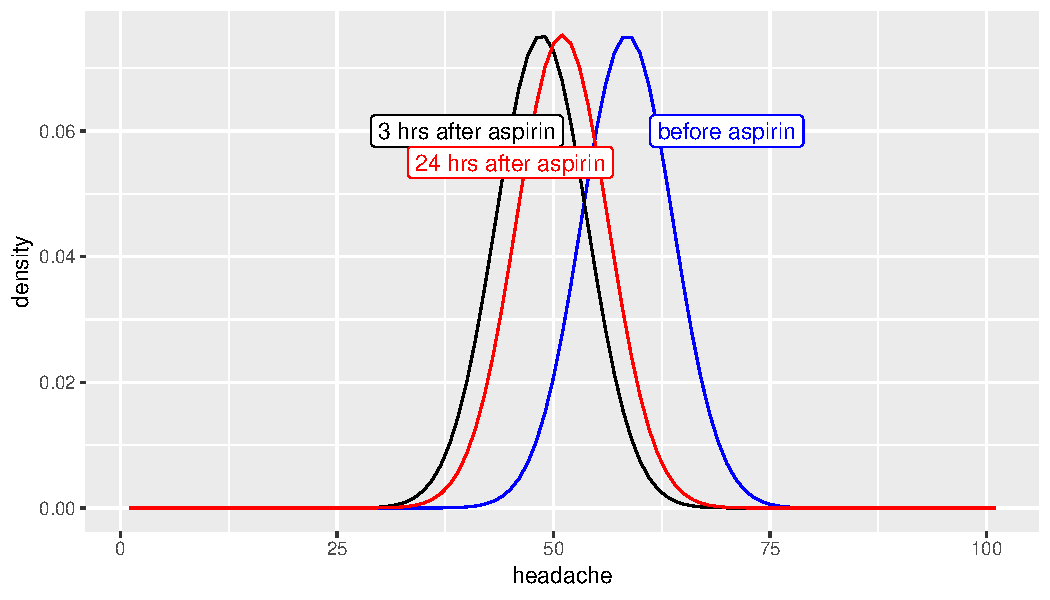
\includegraphics[width=\maxwidth]{figure/analysispremidpost3-1} 

}



\end{knitrout}



So, are these distributions significantly different, in other words, do the means differ significantly before aspirin, 3hrs after aspirin and 24 hrs after aspirin? The answer is yes, because the $F$-test on the group means in the SPSS output is significant. Note the degrees of freedom: 2, because we compare 3 groups of data, so we need two dummy variables. Thus we report that aspirin has an effect on headache levels in NY Times readers, $F(2, 198)=309.58, p<0.001$.

If one has specific hypotheses regarding short-term and long-term effects, one could perform a planned contrast analysis, comparing the first measure with the second measure, and the first measure with the third measure. If one is just interested in whether aspirin has an effect on headache, then the $F$-test should suffice. If apart from this general effect one wishes to explore whether there are significant differences between the three groups of data, without any prior research hypothesis about this, then one could perform a post hoc analysis of the three means. See the relevant chapter on how to perform planned comparisons and post hoc tests.
\\
\\
Now recall that we mentioned an intraclass correlation, or ICC. An intraclass correlation indicates how much clustering there is within the groups, in this case, clustering of headache scores within NY Times readers. How much are the three scores alike that come from the same patient? This correlation can be computed on the basis of the SPSS output, using the following formula:

\begin{eqnarray}
ICC = \frac{\sigma^2_{patient} } {\sigma^2_{patient} +\sigma^2_e }   
\end{eqnarray}

Here, the variance of the \textbf{patient} random effects is equal to 28.3, and the variance of the residuals $e$ is equal to 8.5, so the intraclass correlation for the headache severity scores is equal to 
\begin{eqnarray}
ICC = \frac{28.3} {28.3 + 8.5 } =  0.80
\end{eqnarray}

As this correlation is quite higher than 0, there seems to be quite a lot of clustering. Therefore it's a good thing that we used random effects for the individual differences in headache scores among NY Times readers. Had this correlation been 0 or very close to 0, however, then it would not have mattered to include these random effects. In that case, we might as well use an ordinary linear model, using the UNIANOVA syntax for example. Note from the formula that the correlation becomes 0 when the variance of the random effects for patients is 0.
\\
\\


\subsection{Exercises}

Suppose you let a sample of students do a math test in three different rooms: one with yellow walls, one with red walls and one with blue walls. All students do the math test three times, once in every room. The data are as follows:
\\
 \\
 \begin{tabular}{lrr}
 student & colour & score \\ \hline
 001 & yellow & 60 \\
 001 & red & 66 \\
 001 & blue & 60 \\
 002 & yellow & 24 \\
 002 & red & 15 \\
 002 & blue & 30 \\
 003 & yellow & 90 \\
 003 & red & 90 \\
 003 & blue & 89 \\
 004 & yellow & 10 \\
 004 & red & 20 \\
 004 & blue & 15 \\
 005 & yellow & 23 \\
 005 & red & 13 \\
 005 & blue & 18 \\
 \dots & \dots & \dots \\
 \end{tabular}
\\
\\

\begin{itemize}
\item 1. If you want to test the hypothesis that the colour of the walls do not affect math test scores, and at the same time you want to take into account that some students are generally better at math than others, what would the SPSS syntax be? \\
\item 2. In the output that would result from that syntax from question 1, would you look at a $t$-test or or an $F$-test? Explain your answer.
\item 3. How many degrees of freedom would you see for the denominator?\\
\item 4. Suppose you see this in the output for this colour experiment. How important are the individual difference in math performance in the population of students? Can you quantify the amount of clustering?



\begin{figure}[h]
    \begin{center}
       \includegraphics[scale=0.5]{/Users/stephanievandenberg/Dropbox/Statistiek_Onderwijs/Data" "Analysis/spss" "examples" "mixed" "linear" "model/pre-mid-post" "design/exercise2_correlation.png}
    \end{center}
\end{figure}

\end{itemize}


Answers:
\begin{itemize}
\item 1.
\\
\begin{verbatim}
MIXED score BY colour
  /FIXED=colour
  /PRINT=DESCRIPTIVES  SOLUTION
  /RANDOM=intercept | SUBJECT(student) COVTYPE(VC).
\end{verbatim}

\item 2. $F$-test. There will be two dummy variable and I want to know if the effects of both of these are significantly different from 0. The $t$-tests  give me only information about the dummy variables separately. \\
\item 3. 2, because there are 3 different colours, which can be represented by 2 dummy-variables. \\
\item 4. In the table with the data you generally see that students who score high in one room also score high in another room (for instance, students 001 and 003). Students who score low in one room also score low in another room (for instance students 002, 004 and 005). This clustering can be quantified using an intraclass correlation, in this case equal to $\frac{228}{228+270}=0.46$. 
\end{itemize}


\section{Pre-mid-post intervention design: linear effects}
In the previous section, we've looked at \textit{qualitative} variables: \textbf{measure} (pre intervention, 3 hours after, and 24 hours after), or \textbf{colour} (yellow, red, and blue rooms). We can use the same type of analysis for \textit{quantitative} variables. In fact, we could have used a linear effect for time in the headache example: using time of measurement as a variable. Let's look at the headache data again. But now we've created a new variable \textbf{time} that is based on the measure \textbf{variable}: all first measurements are coded as \textbf{time}=0, all second measurements after 3 hours are coded as \textbf{time}=3, and all third measurements after 24 hours are coded as \textbf{time}=24.

\begin{knitrout}
\definecolor{shadecolor}{rgb}{0.969, 0.969, 0.969}\color{fgcolor}
\begin{tabular}{r|r|r|r}
\hline
patient & measure & headache & time\\
\hline
1 & 1 & 52 & 0\\
\hline
1 & 2 & 45 & 3\\
\hline
1 & 3 & 47 & 24\\
\hline
2 & 1 & 59 & 0\\
\hline
2 & 2 & 50 & 3\\
\hline
2 & 3 & 55 & 24\\
\hline
3 & 1 & 65 & 0\\
\hline
3 & 2 & 56 & 3\\
\hline
3 & 3 & 58 & 24\\
\hline
4 & 1 & 51 & 0\\
\hline
\end{tabular}


\end{knitrout}
 
 
Instead of using a qualitative variable intervention, with three levels, we now use a quantitative variable, time, indicating the number of hours that have elapsed after aspirin intake. At point 0 hours, we measure headache severity, and patients take an aspirin. Next we measure headache after 3 hours and 24 hours. Above, we wanted to know if there were differences in average headache between before intake and 3hrs and 24 hrs after intake. Another question we might ask ourselves: is there a \textit{linear} reduction in headache severity after taking aspirin?

For this we can do a linear regression type of analysis. We want to take into account individual differences in headache severity levels among patients, so we perform a MIXED analysis in SPSS, using the following syntax, replacing the key word BY with WITH, and the variable \textbf{measure} by \textbf{time}:

\begin{verbatim}
MIXED headache WITH time
  /FIXED=time
  /PRINT=DESCRIPTIVES  SOLUTION
  /RANDOM=intercept | SUBJECT(patient) COVTYPE(VC).
\end{verbatim}


Below we see the corresponding output:

\begin{figure}[h]
    \begin{center}
       \includegraphics[scale=0.8, trim={0cm 20cm 0cm 0cm} ]{/Users/stephanievandenberg/Dropbox/Statistiek_Onderwijs/Data" "Analysis/spss" "examples" "linear" "mixed" "model/premidpost/premidpostaspirinlinear.pdf}
    \end{center}
\end{figure}


Based on the output, we see that the model for our data is equivalent to


\begin{eqnarray}
headache_{ij} = 54 + patient_i - 0.16 \times time + e_{ij} \\
patient_i \sim N(0, 21)\\
e_{ij} \sim N(0, 31)
\end{eqnarray}

This model predicts that at time 0, the average headache severity score equals 54, and that for every hour after intake, the headache level drops by 0.16 points. So it predicts for example that after 10 hours, the headache has dropped 1.6 points to 52.4. 
\\
\\
Is this a good model for the data? Probably not, look at the variance of the residuals: with its 31 it is now a lot bigger than in the previous analysis with the same data (see previous section). Larger variance of residuals means that the model explains the data worse: predictions are worse, so the residuals increase in size. 
\\
\\
That the model is not appropriate for this data set is also obvious when we plot the data, focusing on the relationship between time and headache levels:


\begin{knitrout}
\definecolor{shadecolor}{rgb}{0.969, 0.969, 0.969}\color{fgcolor}

{\centering 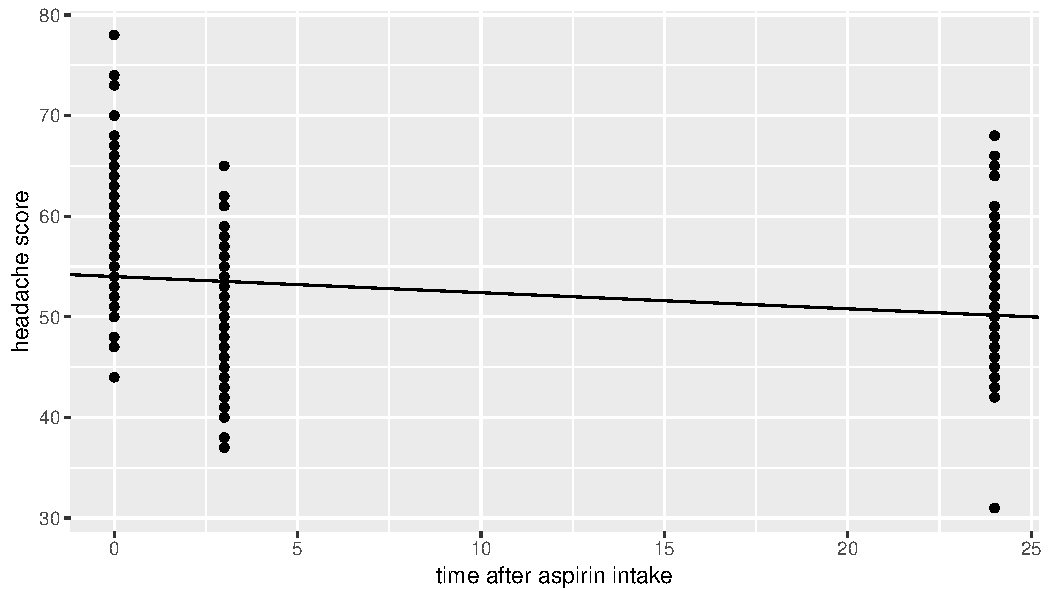
\includegraphics[width=\maxwidth]{figure/analysispremidpost5-1} 

}



\end{knitrout}

The line shown is the fitted line based on the SPSS output. It can be seen that the prediction for time=0 is too low, for time=2 too high, and for time=24 again too low. So for this particular data set on headache, it would be better to use a qualitative predictor for the effect of time on headache, like we did in the previous section.
\\
\\
As an example of a data set where a linear effect would have been appropriate, imagine that we measured headache 2 hours and 3 hours after aspirin intake (but not after 24 hours). Suppose these data would look like this:


\begin{knitrout}
\definecolor{shadecolor}{rgb}{0.969, 0.969, 0.969}\color{fgcolor}

{\centering 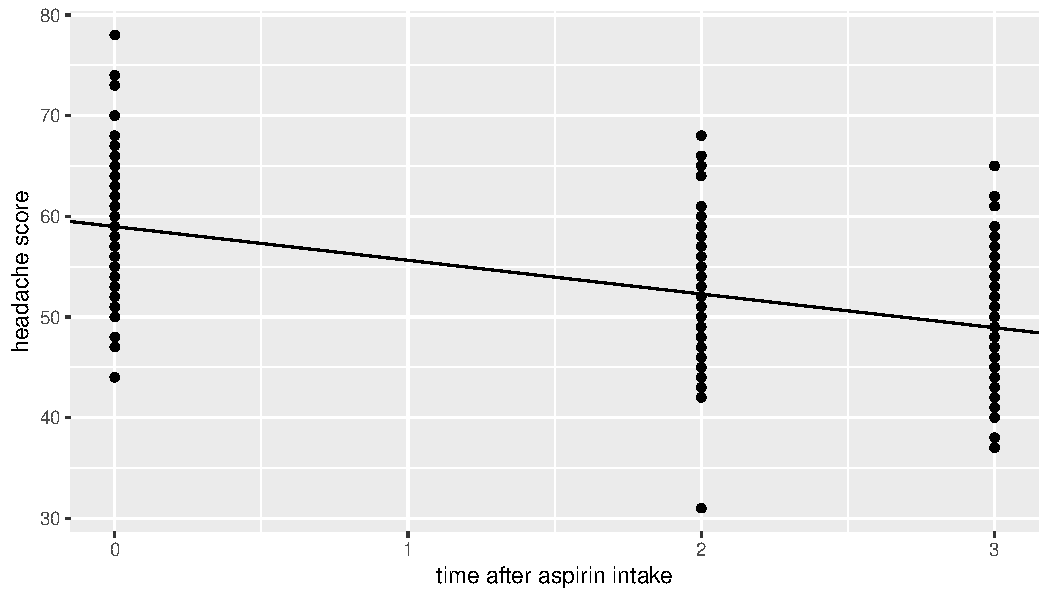
\includegraphics[width=\maxwidth]{figure/analysispremidpost6-1} 

}



\end{knitrout}

Here we see a gradual increase of headache levels right after aspirin intake. Here, a quantitative treatment of the time variable would be more appropriate. The SPSS output is given below.


\begin{figure}[h]
    \begin{center}
       \includegraphics[scale=0.8, trim={0cm 20cm 0cm 0cm} ]{/Users/stephanievandenberg/Dropbox/Statistiek_Onderwijs/Data" "Analysis/spss" "examples" "linear" "mixed" "model/premidpost/premidpostaspirinlinear2.pdf}
    \end{center}
\end{figure}


From the output we see that the intercept is 59 and that the slope is -3.3. So this model predicts an hourly decrease of 3.3 points in headache level. This regression line is also depicted in the above figure. 

Because we are confident that this model is appropriate for our data, we can interpret the statistical output from SPSS. 

\begin{quotation}
A linear mixed model was run, using a quantitive variable time and random effects for the variable patient. We saw a significant linear effect of time on headache level, $t(199)=-24.42, p < 0.001$. The estimated effect of time based on this analysis is negative, $-3.3$, so with every hour that elapses after aspirin intake, the predicted headache score decreases with 3.3 points. 
\end{quotation}


\subsection{Exercises}

Suppose you have a number of CEOs with smart watches and you have these smart watches log skin conductance. Skin conductance is a good measure for stress. These measurements are done at random intervals, for at most 4 times during one day. The experiment starts at 7am and stops at 7pm. The \textbf{time} variable measures how many hours have passed since 7am.
 \\
 \\
 \begin{tabular}{lrr}
 CEO & time & conductance \\ \hline
 001 & 2 & 80 \\
 001 & 3 & 65 \\
 001 & 10 & 60 \\
 001 & 11 & 60 \\
 002 & 4 & 34 \\
 002 & 6 & 25 \\
 002 & 9 & 30 \\
 002 & 12 & 30 \\
 003 & 3 & 23 \\
 003 & 4 & 15 \\
 003 & 5 & 20 \\
 003 & 8 & 20 \\
 004 & 0 & 90 \\
 004 & 3 & 70 \\
 004 & 4 & 65 \\
 004 & 11 & 65 \\
 \dots & \dots & \dots \\
 \end{tabular}
\\
\\
Now you'd like to know if skin conductance in CEOs shows a general decrease during the day. Your null-hypothesis is therefore that there is no linear effect of time on skin conductance. Now, you have multiple measures for each CEO (repeated measures), and there might be individual differences in the average skin conductance that you would like to take into account. Therefore you perform a MIXED analysis in SPSS. 

\begin{itemize}
\item 1. What would the SPSS syntax look like? \\
\item 2. If you got the following output, what would your predicted skin conductance be for a CEO at 15.00 hrs? \\
\begin{figure}[h]
    \begin{center}
       \includegraphics[scale=0.5]{/Users/stephanievandenberg/Dropbox/Statistiek_Onderwijs/Data" "Analysis/spss" "examples" "mixed" "linear" "model/pre-mid-post" "design/CEOexample.png}
    \end{center}
\end{figure}



\item 3. Look at the data plotted: do you think a linear effect is reasonable for this data set?

\begin{knitrout}
\definecolor{shadecolor}{rgb}{0.969, 0.969, 0.969}\color{fgcolor}

{\centering 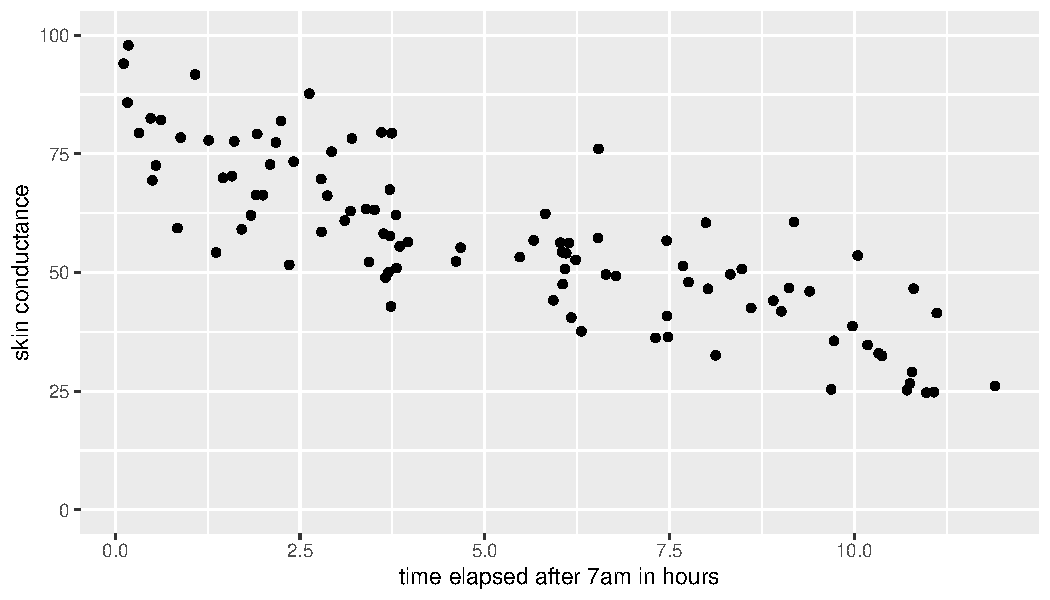
\includegraphics[width=\maxwidth]{figure/analysispremidpost7-1} 

}



\end{knitrout}




\item 4. How much clustering is there for skin conductance across CEOs? \\
\item 5. Would you say these individual differences are very important to take into account? \\
\item 6. Is there a significant effect of time of day on skin conductance in CEOs?\\
\item 7. What is the effect of time of day on skin conductance in CEOs? Also give the 95\% confidence interval of this effect.
\item 8. Write a short paragraph that describes the results in APA format.
\item 9. Given a new data set where every student's mood was tested at three points in time: During Christmas holidays (time points 1), during Easter holidays (time point 2) and at the start of the academic year, September 1 (time point 3). Look at the data plotted: do you think a linear effect is reasonable for this data set? Explain your answer.

\begin{knitrout}
\definecolor{shadecolor}{rgb}{0.969, 0.969, 0.969}\color{fgcolor}

{\centering 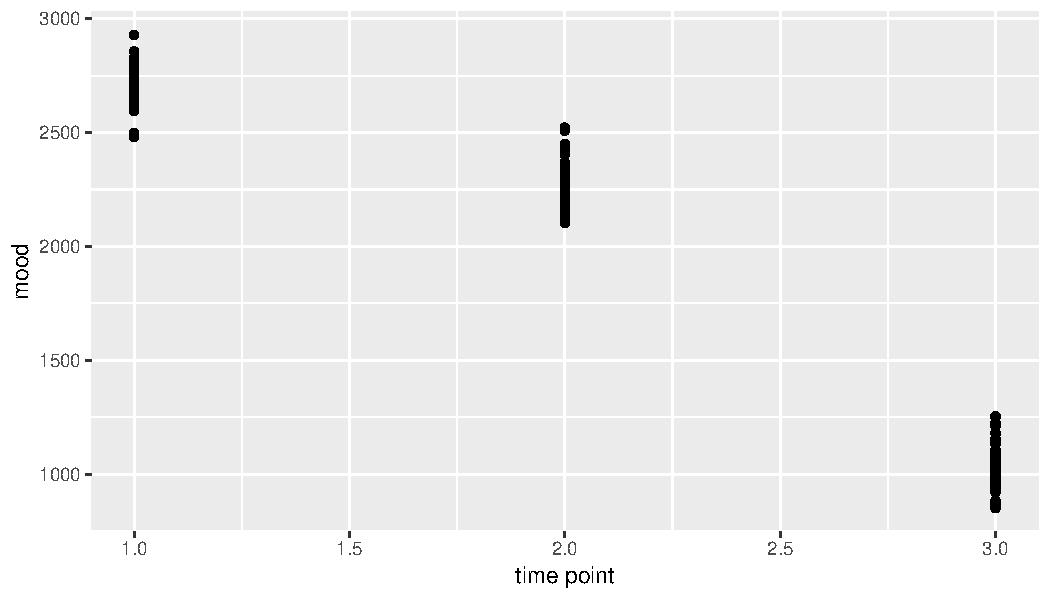
\includegraphics[width=\maxwidth]{figure/analysispremidpost8-1} 

}



\end{knitrout}

\item 10. Provide the syntax you would use to analyse the problem of question 9.


\end{itemize}

Answers:
\begin{itemize}
\item 1. \\
\begin{verbatim}
MIXED conductance WITH time
  /FIXED=time
  /PRINT=DESCRIPTIVES  SOLUTION
  /RANDOM=intercept | SUBJECT(CEO) COVTYPE(VC).
\end{verbatim}
\item 2. 15 hrs is equal to 8 hours after 7am, so the expected skin conductance is equal to $62 - 4 \times 8= 30$\\
\item 3. Yes, a general linear downward trend is observed for the skin conductance.
\item 4. The intraclass correlation coefficient is equal to $\frac{235}{235+247}=0.49$, 
\item 5. The correlation is quite different from 0, so there is certainly some clustering in the data and it is important to take these individual differences into account. \\
\item 6. Yes, there is a signficant linear effect of time on skin conductance in CEOs, $t(59)=-4.24, p < 0.01$.\\
\item 7. The linear effect of time of day on skin conductance in CEOs is around -4.13 points per hour after 7am (95 \% CI: -6.08 -- -2.18). \\
\item 8. \begin{quotation}
        A linear mixed model was run with time as a quantitative predictor for skin conductance, including random effects for CEO. We found an effect of time of -4.13 points per hour which was significantly different from 0, $t(59)=-4.24, p < 0.001$. Therefore we conclude that time of day has an effect on skin conductance in the entire population of CEOs.
        \end{quotation}
        
\item 9. The relationship is not linear: you cannot draw a straight line through the means of the three measurements. 
\item 10. Because we have multiple measurements from the same students we should use a MIXED analysis. Furthermore, a qualitave analysis would be more suitable, given the nonlinear relationship between time and mood. So we use the syntax:

\begin{verbatim}
MIXED mood BY time
  /FIXED=time
  /PRINT=DESCRIPTIVES  SOLUTION
  /RANDOM=intercept | SUBJECT(student) COVTYPE(VC).
\end{verbatim}

\end{itemize}



\section{Linear mixed models and interaction effects}


Suppose we carry out the aspirin and headache study not only with a random sample of NY Times readers that suffer from regular headaches, but also with a random sample of readers of the Wall Street Journal that suffer from regular headaches. We'd like to know whether aspirin works, but we are also interested to know whether the effect of aspirin is similar in the two groups of readers. Our null-hypothesis is that the effect of aspirin in affecting headache severity is the same in NY Times and Wall Street Journal readers that suffer from headache.\\
\\
H\_0: The effect of aspirin is the same for NY Times readers as for Wall Street Journal readers.
\\
\\
Suppose we have the following data set (we only show the first six patients), and we only look at the measurements before aspirin intake and 3 hours after aspirin intake (pre-post design):

\begin{knitrout}
\definecolor{shadecolor}{rgb}{0.969, 0.969, 0.969}\color{fgcolor}
\begin{tabular}{r|l|r|r}
\hline
patient & group & pre & post\\
\hline
1 & NYTimes & 55 & 45\\
\hline
2 & WallStreetJ & 63 & 50\\
\hline
3 & NYTimes & 66 & 56\\
\hline
4 & WallStreetJ & 50 & 37\\
\hline
5 & NYTimes & 63 & 50\\
\hline
6 & WallStreetJ & 65 & 53\\
\hline
\end{tabular}


\end{knitrout}



In this part of the data set, patients 2, 4, and 6 read the Wall Street Journal, and patients 1, 3 and 5 read the NY Times. We assume that people only read one of these newspapers. We measure their headache before and after the intake of aspirin (a pre-post design). The data are now in what we call \textit{wide format}: the dependent variable \textbf{headache} is spread over two columns, \textbf{pre} and \textbf{post}. In order to analyse the data with linear models, we need them in \textit{long format}, like this:

\begin{knitrout}
\definecolor{shadecolor}{rgb}{0.969, 0.969, 0.969}\color{fgcolor}
\begin{tabular}{r|l|r|r}
\hline
patient & group & measure & headache\\
\hline
1 & NYTimes & 1 & 55\\
\hline
1 & NYTimes & 2 & 45\\
\hline
2 & WallStreetJ & 1 & 63\\
\hline
2 & WallStreetJ & 2 & 50\\
\hline
3 & NYTimes & 1 & 66\\
\hline
3 & NYTimes & 2 & 56\\
\hline
\end{tabular}


\end{knitrout}


The new variable \textbf{measure} now indicates whether a given measurement of headache refers to a measurement before intake (first measurement) or after intake (second measurement). Again we could investigate whether there is an effect of aspirin with a linear mixed model, with \textbf{measure} as our qualitative predictor, but that is not really what we want to test: we only want to know whether the effect of aspirin (being small, large, negative or non-existent) \textit{is the same for both groups}. Remember that this hypothesis states that there is no interaction effect of aspirin (\textbf{measure}) and group. The null-hypothesis is that group is \textit{not} a moderator of the effect of aspirin on headache. There may be an effect of aspirin or there may not, and there may be an effect of newspaper (\textbf{group}) or there may not, but we're interested in the \textit{interaction} of aspirin and group membership. Is the effect of aspirin different for NY times readers than for Wall Street Journal readers?

In our analysis we therefore need to specify an interaction effect. Since the data are clustered (2 measures per patient), we use a linear \textit{mixed} model. First we show how to analyse these data using dummy variables, later we will show the results using a different approach. 
\\
\\
We recode the data into two dummy variables, one for the aspirin intervention (measure), and one for group membership. 

\begin{verbatim}
RECODE measure (1=0) (2=1) INTO post.
RECODE group ('WallStreetJ'=0) ('NYTimes'=1) INTO NYTimes.
EXECUTE.
\end{verbatim}

Next we need to compute the product of these two dummies to code for the interaction effect. Since with the above dummy coding, all post measures get a 1, and all NYTimes readers get a 1, only the observations that are post aspirin and that are from NYTimes readers get a 1 for the product, the interactiondummy . That's why it is best to name this interaction effect PostNYTimes. 

\begin{verbatim}
COMPUTE PostNYTimes=post*NYTimes.
EXECUTE.
\end{verbatim}

With these three new dummy variables we can specify the linear mixed model.

\begin{verbatim}
MIXED headache WITH post NYTimes PostNYTimes
  /FIXED= post NYTimes PostNYTimes
  /PRINT=DESCRIPTIVES  SOLUTION
  /RANDOM=intercept | SUBJECT(patient) COVTYPE(VC).
\end{verbatim}


In the output below, we recognize the three fixed effects for the three dummy variables. Since we're interested in the interaction effect, we look at the effect of PostNYTimes. The effect is in the order of +0.6. So what does this mean? 

\begin{figure}[h]
    \begin{center}
       \includegraphics[scale=0.8, trim={0cm 19cm 0cm 0cm}]{/Users/stephanievandenberg/Dropbox/Statistiek_Onderwijs/Data" "Analysis/spss" "examples" "linear" "mixed" "model/mixedprepost/mixedprepostdummy.pdf}
    \end{center}
\end{figure}



Remember that a reader from the Wall Street Journal gets a 0 for the group dummy \textbf{NYTimes}. All headache measures before aspirin intake are given a 0 for the intervention dummy \textbf{post}. 
Since the product of $ 0\times 0$ equals 0, all these measures before aspirin in Wallstreet Journal readers get a 0 for the interaction dummy \textbf{PostNYTimes}.
Therefore, the intercept of 59.5 refers to the expected headache severity of Wall Street Journal readers \textit{before} they take their aspirin. This is significantly different from zero, meaning that in the population of Wall Street Journal readers, headache before aspirin intake is different from zero.

Furthermore, we see that the effect of the intervention is -10.7. So, relative to Wall Street Journal readers prior to aspirin intake, the level of post intake headache is 10.7 points \textit{less}. So in the population of Wall Street Journal readers, the effect of aspirin is different from 0, since the effect of -10.7 is significant. 

If we look further down in the table, we see the effect of NYTimes equals 0.32. So, relative to Wall Street Journal readers, before aspirin intake (the reference group), NY Times readers score on average 0.32 points higher on the headache scale before aspirin intake. 

However, we're not interested in a general difference between those two groups of readers, we're interested in the effect of aspirin and whether it is different in the two groups of readers. In the last row we see the interaction effect: being a reader of the NY Times AND at the same time being a measure after aspirin intake, the expected increase in mean headache equals 0.60. So the effect of aspirin is -10.7 in Wall Street Journal readers, as we saw above, but the  effect is $-10.7 + 0.6 = -10.1$ in NY Times readers. So in this sample the effect of aspirin on headache is 0.6 \textit{smaller} than in Wall Street Journal readers (note that even while the interaction effect is positive, it is positive on a scale where a high score means more headache). 


Let's look at it in the different way, using a table with the dummy codes. For each group of data, pre or post aspirin and New York Times readers and Wall Street Journal readers, we note the dummy codes for the new dummy variables. In the last column we use the output estimates and multiply them with the respective dummy codes (1 and 0) to obtain the expected headache level (using rounded numbers):
\\
 \\
 \begin{tabular}{llrrrr}
  measure & group & post & NYTimes & PostNYT & exp mean \\ \hline
  pre   & WallStreet      &  0 & 0 & 0 & $60$ \\
 post   &  WallStreet     &  1 & 0 & 0 & $60 + (-11)=49$ \\
 pre    & NYtimes         &  0 & 1 & 0 & $60 + 0.3=60.3$  \\
 post   &  NYtimes        &  1 & 1 & 1 & $60 +(-11) + 0.3 + 0.6=49.9$ \\
 \end{tabular}
\\
\\
The exact numbers are displayed in the graph below:

\begin{knitrout}
\definecolor{shadecolor}{rgb}{0.969, 0.969, 0.969}\color{fgcolor}

{\centering 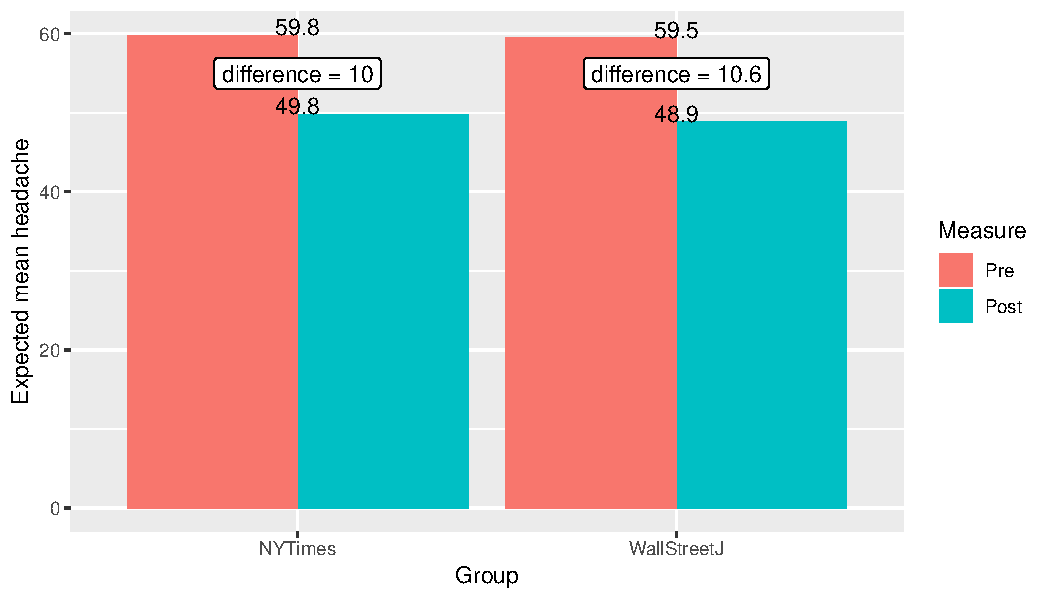
\includegraphics[width=\maxwidth]{figure/analysisprepostmixed3-1} 

}



\end{knitrout}


We see that the specific effect of aspirin in NYTimes readers is 0.6 smaller than the effect of aspirin in Wall Street Journal readers. This difference in the effect of aspirin between the groups was not significantly different from 0. The null-hypothesis that the effect is the same in the two populations of readers cannot be rejected. We therefore conclude that the effect that aspirin has on patients is the same for NY Times and Wall Street Journal readers. 

Note that we could have done the analysis in another way, not treating the variables in a quantitative way and using dummy variables, but by treating them qualitatively using the key word BY. The SPSS syntax would then be:

\begin{verbatim}
MIXED headache BY measure group 
  /FIXED=measure group measure*group
  /PRINT=DESCRIPTIVES  SOLUTION
  /RANDOM=intercept | SUBJECT(patient) COVTYPE(VC).
\end{verbatim}


The output would then look like below:


\begin{figure}[h]
    \begin{center}
       \includegraphics[scale=0.8, trim={0cm 15cm 0cm 0cm}]{/Users/stephanievandenberg/Dropbox/Statistiek_Onderwijs/Data" "Analysis/spss" "examples" "linear" "mixed" "model/mixedprepost/mixedprepostquali.pdf}
    \end{center}
\end{figure}



Here SPSS has automatically created dummy variables, one for \textbf{measure=1}, one for \textbf{group=1}, and one for the interaction effect, \textbf{group=1 AND measure=1}. Because the dummy coding is different, the intercept and the main effects of group and measure have changed, but you see that the interaction effect is still 0.6, albeit now negative. We also see that the significance level of the interaction effect is still the same. You are always free to choose to either construct your own dummy variables and analyze them in a quantitative way (using WITH), or to let SPSS construct the dummy variables for you (using BY): the $p$-value for the interaction effect will always be the same (this is not true for the intercept and the main effects).

Because the two analyses are equivalent (they end up with exactly the same predictions, feel free to check!), we can safely report that we've found a nonsignificant group by measure interaction effect, $t(98)=0.74, p=0.46$. We therefore conclude that in the populations of NY Times readers and Wall Street Journal readers, the short-term effect of aspirin on headache is the same. 



\subsection{Exercises}

Below we see data from a study on the effects of the financial crisis on the number of employees in specific Dutch companies. The companies are distinguised into food and non-food related companies. The number of employees are recorded in January 2008 and January 2011.

\begin{knitrout}
\definecolor{shadecolor}{rgb}{0.969, 0.969, 0.969}\color{fgcolor}
\begin{tabular}{r|l|r|r}
\hline
company & food & 2008 & 2011\\
\hline
1 & nonfood & 42 & 63\\
\hline
2 & food & 104 & 126\\
\hline
3 & nonfood & 76 & 58\\
\hline
4 & food & 65 & 131\\
\hline
\end{tabular}


\end{knitrout}

\begin{enumerate}
\item These data are in wide format. Rewrite the datamatrix in such a way that we have the same data in long format. Provide column (variable) names. 
\\
 \\
 \begin{tabular}{llrrrr}
   & \dots & \dots  & \dots & \dots  & \dots  \\ \hline
  & \dots & \dots  & \dots & \dots  & \dots  \\
  & \dots & \dots  & \dots & \dots  & \dots  \\
  & \dots & \dots  & \dots & \dots  & \dots  \\
  & \dots & \dots  & \dots & \dots  & \dots  \\
  & \dots & \dots  & \dots & \dots  & \dots  \\
  & \dots & \dots  & \dots & \dots  & \dots  \\
  & \dots & \dots  & \dots & \dots  & \dots  \\
  & \dots & \dots  & \dots & \dots  & \dots  \\
  & \dots & \dots  & \dots & \dots  & \dots  \\
  & \dots & \dots  & \dots & \dots  & \dots  \\
  & \dots & \dots  & \dots & \dots  & \dots  \\
  & \dots & \dots  & \dots & \dots  & \dots  \\
 \end{tabular}
\\
\\
\item Do we need to use a linear mixed model, or can we analyse these data with an ordinary linear model?
\item We want to test the null-hypothesis that the effects of the financial crisis in 2008 has the same effect on the number of employees in the food sector as in the non-food sector. Provide the syntax that helps you test this hypothesis. 
\item Suppose the following output results from an analysis done by a colleague:

\begin{figure}[h]
    \begin{center}
       \includegraphics[scale=0.8, trim={0cm 15cm 0cm 0cm}]{/Users/stephanievandenberg/Dropbox/Statistiek_Onderwijs/Data" "Analysis/spss" "examples" "linear" "mixed" "model/mixedprepost/mixedprepostemployee.pdf}
    \end{center}
\end{figure}

She provides you with the information that food=1 means the food sector and food=2 is the nonfood sector.

What does the model predict regarding the number of employees in 2008 in the non-food sector?
\item What does the model predict regarding the number of employees in 2011 in the non-food sector?
\item What does the model predict regarding the number of employees in 2008 in the food sector?
\item What does the model predict regarding the number of employees in 2011 in the food sector?
\item How large is the effect of the crisis in the food sector?
\item How large is the effect of the crisis in the non-food sector
\item How large is the intraclass correlation (ICC)? Give the computation.
\item Could we have done the analysis with an ordinary linear model? Explain your answer.
\item Can we reject the null-hypothesis that the effects of the crisis were the same in the food and non-food sectors? Explain your answer.
\end{enumerate}


Answers:
\\
\begin{enumerate}
\item It could look like this:
\\
\\
\begin{tabular}{llrrrr}
   & company & sector  & year & NEmployees  & \dots  \\ \hline
  & 1 & nonfood  & 2008 & 42  & \dots  \\
  & 1 & nonfood  & 2011 & 63  & \dots  \\
  & 2 & food  & 2008 & 104  & \dots  \\
  & 2 & food  & 2011 & 126  & \dots  \\
  & 3 & nonfood  & 2008 & 76  & \dots  \\
  & 3 & nonfood  & 2011 & 58  & \dots  \\
  & 4 & food  & 2008 & 65  & \dots  \\
  & 4 & food  & 2011 & 131  & \dots  \\
\end{tabular}
\\
\\
\item The data are clustered into companies: for each company we have two data points, so we should at least try a linear mixed model. Only if the variance of the company random effects is extremely small, we could use a linear model without random effects.
\item One option is to let SPSS construct the dummy variables:

\begin{verbatim}
MIXED employees BY year sector 
  /FIXED=year sector year*sector
  /PRINT=DESCRIPTIVES  SOLUTION
  /RANDOM=intercept | SUBJECT(company) COVTYPE(VC).
\end{verbatim}

Or you do the dummy coding yourself, for example like this:

\begin{verbatim}

RECODE year (2008=0) (2011=1) INTO year2011.
RECODE sector ('Nonfood'=0) ('food'=1) INTO food.
EXECUTE.

COMPUTE food2011=year2011*food.
EXECUTE.

MIXED employees WITH year2011 food food2011
  /FIXED= year2011 food food2011
  /PRINT=DESCRIPTIVES  SOLUTION
  /RANDOM=intercept | SUBJECT(company) COVTYPE(VC).
\end{verbatim}

\item the nonfood sector is food=2, so the predicted number of employees in 2008 in the nonfood sector is equal to $81.57 + 0 -22.056 + 0= 59.514$
\item the nonfood sector is food=2, so the predicted number of employees in 2011 in the nonfood sector is equal to $81.57 + 0 + 0 + 0= 81.57$
\item the food sector is food=1, so the predicted number of employees in 2008 in the food sector is equal to $81.57 + 39.31 -22.056 + 0.85=99.674 $
\item the food sector is food=1, so the predicted number of employees in 2011 in the food sector is equal to $81.57 + 39.31 + 0 + 0 = 120.88   $ 
\item in the food sector the effect is a $120.88 - 99.674 =   21.206$ increase in number of employees
\item in the non-food sector the effect is a $81.57 - 59.514 =   22.056$ increase in number of employees
\item the ICC is $\frac{12}{12+208}=0.05$
\item we have clustering, with multiple data point per company, so in general a linear mixed model is better than an ordinary linear model. However, since the intraclass correlation is rather low, the results would be very similar if we would use an ordinary linear model.
\item The null-hypothesis cannot be reject as the year by sector interaction effect is not signifcantly different from 0, $t(998)=0.66, p=0.51$. (alternatively, $F(1,998)=0.44, p=0.51$). Note however that the statistical results are in terms of absolute number of employees. These data show that the average number of employees in 2008 is larger in the food sector than in the non-food sector. Perhaps it would be wiser to look at percentage increase in number of employees: A change from 100 to 102 reflects a larger impact than a change from 1000 to 1002.

\end{enumerate}





\section{Mixed designs}
The design in the previous section where we had both a grouping variable and a pre-post or repeated measures design, is often called a \textit{mixed design}. It is a mixed design in the sense that there are two kinds of variables: one is a \textit{between-individuals} variable, and one variable is a \textit{within-individual} variable. Here the between-individuals variable is \textbf{group}: two different populations of readers. It is called \textit{between} because one individual can only be part of one group. When we study the effect of the group effect we are essentially comparing the scores of one group of individuals with the scores of another group of individuals, so the comparison is \textit{between different individuals}. 
The two groups of data are said to be \textit{independent}, as we knew that none of the readers in this data set reads both journals. 

The within-variable in this design is the aspirin intervention, indicated by the variable \textbf{measure}. For each individual we have two observations: all individuals are present in both the pre condition data as well as in the post condition data. With this intervention variable, we are comparing the scores of a group of indiviudals with the scores \textit{of that same group of individuals} at another time point. The comparison of scores is within a particular individual, at timepoint 1 and at timepoint 2. So the pre and post sets of data are not independent: the headache scores in both conditions are coming from the same individuals. 

Mixed designs are often seen in psychological experiments. For instance, you want to know how large the effect of alcohol intake is on driving performance. You want to know whether the effect of alcohol on driving performance is the same in a Fiat 600 as in a Porsche. Suppose you have 100 participants for your study. There are many choices you can make regarding the design of your study. Here we discuss 4 alternative research designs:

\begin{enumerate}


\item One option is to have all participants participate in all four conditions: they all drive a Fiat with and without alcohol, and they all drive a Porsche, with and without alcohol. In this case, both the car and the alcohol are within-participant variables.

\item The second option is to have 50 participants drive a Porsche, with and without alcohol, and to have the other 50 participants drive the Fiat, with and without alcohol. In this case, the car is the between-participants variable, and alcohol is the within-participant variable. 

\item The third option is to have 50 participants without alcohol drive both the Porsche and the Fiat, and to have the other 50 participants drive the Porsche and the Fiat with alcohol. Now the car is the within-participant variable, and the alcohol is the between-participants variable.

\item The fourth option is to have 25 participants drive the Porsche with alcohol, 25 other participants drive the Porsche without alcohol, 25 participants drive the Fiat with alcohol, and the remaining 25 participants drive the Fiat without alcohol. Now both the car variable and the alcohol variable are between-participant variables: none of the participants is present in more than 1 condition.

\end{enumerate}

Only the second and the third design described here are mixed designs, having at least one between-participants variable and at least one within-participant variable. 

Remember that when there is at least one within variable in your design, you have to use a linear mixed model. If all variables are between variables, one can use an ordinary linear model. Note that the term \textit{mixed} in linear mixed model refers to the effects in the model that can be both random and fixed. The term \textit{mixed} in mixed designs refers to the mix of two kinds of variables: within variables and between variables. 

Also note that the within and between distinction refers to the units of analysis. If the unit of analysis is school, then the location of the school building is a between-school variable. An example of a within-school variable could be time: before a major curriculum reform and after a major curriculum reform. 

\subsection{Exercises}

\begin{enumerate}
\item A psychologist studies whether age affects math performance. In 2017, she measures math performance (one score) in a group of 80-year-olds and she measures math performance (one score) in a group of 90-year-olds. \\
1. In this design, is the age variable a between-participants variable or a within-participant variable?  \\
2. Would you analyze these data with a linear model, or with a linear mixed model? Explain. 
\\
\\
\item A psychologist studies whether age affects math performance. She measures math performance (one score) in a group of 7-year-olds and she measures math performance again when the same children are 8 years old. \\
1. In this design, is the age variable a between-participants variable or a within-participant variable?  \\
2. Would you analyze these data with a linear model, or with a linear mixed model? Explain. 
\\
\\
\item Look at the data table below.
\\
 \\
 \begin{tabular}{rllr}
  ID & Nationality & Sex & Mathscore  \\ \hline
  1   & Dutch      &  Male & 67   \\
 2   &  Dutch     &  Female & 88   \\
 3    & German         &  Male & 50   \\
 4   &  German        &  Female & 98  \\
  \dots   & \dots        &  \dots& \dots  \\
 \end{tabular}
\\
\\
In this data set on Math performance, we see two variables, nationality and sex. What kind of variables are these: within-participant variables or between-participants variables? Explain.
\\
1. Would you call this a mixed design? Explain.\\
2. Would you analyze this data set with a linear model or with a linear mixed model? Explain.
\\
\\
\item Look at the data table below.
\\
 \\
 \begin{tabular}{rllr}
  ID & Nationality & Age & Mathscore  \\ \hline
  1   & Dutch      &  3 & 67   \\
 1   &  Dutch     &  5 & 88   \\
 2    & German         &  4 & 50   \\
 2   &  German        &  6 & 98  \\
  \dots   & \dots        &  \dots& \dots  \\
 \end{tabular}
\\
\\
In this data set on Math performance, we see two variables, nationality and age. What kind of variables are these: within-participant variables or between-participants variables? Explain.\\
1. Would you call this a mixed design? Explain.\\
2. Would you analyze this data set with a linear model or with a linear mixed model? Explain.
\\
\\
\item Look at the data table below.
\\
 \\
 \begin{tabular}{rllr}
  ID & Subject & Sex & Mood  \\ \hline
  1   & Psychology      &  Male & 67   \\
 1   &  Psychology     &  Female & 88   \\
 2    & Sociology         &  Female & 50   \\
 2   &  Sociology        &  Male & 98  \\
  \dots   & \dots        &  \dots& \dots  \\
 \end{tabular}
\\
\\
In this data set on mood in transsexuals, we see two variables, the subject they have a Master's degree in, and sex. What kind of variables are these: within-participant variables or between-participants variables? Explain.\\
1. Would you call this a mixed design? Explain.\\
2. Would you analyze this data set with a linear model or with a linear mixed model? Explain.\\
\\
\item Look at the data table below.
\\
 \\
 \begin{tabular}{lrrr}
  SchoolID & Country & Year & Avarage Mathscore  \\ \hline
 1   & The Netherlands      &  2010 & 67   \\
 1   &  The Netherlands     &  2011 & 88   \\
 1    & The Netherlands         &  2012 & 50   \\
 1   &  The Netherlands        &  2013 & 98  \\
 2   & Germany      &  2010 & 67   \\
 2   &  Germany     &  2011 & 88   \\
 2    & Germany         &  2012 & 50   \\
 2   &  Germany        &  2013 & 98  \\
  \dots   & \dots        &  \dots & \dots  \\
 \end{tabular}
\\
\\
In this data set on average Math performance in schools, we see two variables, country of the school and year of data collection. What kind of variables are these: within-school variables or between-schools variables? Explain.\\
1. Would you call this a mixed design? Explain.\\
2. Would you analyze this data set with a linear model or with a linear mixed model? Explain.\\

\end{enumerate}


Answers:

\begin{enumerate}

\item 

1. The age variable is a between-participants variable: some of the participants are 80 years old and some are 90 years old: none are both at the same time. Age discriminates between two sets of participants, so it is a between-participants variable.
2. Two groups of participants were studied. Because we only have one measure for each participant, there is no clustering, and we use an ordinary linear model.


\item
1. The age variable is a within-participants variable: children are studied twice and scores can therefore be compared within an individual.
2. One group of participants was studied and for each participant we have two math scores. Because we have more than one measure for each participant, we have to use a linear mixed model to account for clustering.

\item 
Each participant is either Dutch or German. This is a between-participants variable. Each participant is either male or female, sex discriminates between separate groups of participants, so sex is a between-participants variable.
1. This is \textit{not} a mixed design as it does not have both within-participant and between-participants independent variables. 
2. Because we only have one measure for each participant, there is no clustering, and we use an ordinary linear model.


\item 
Each participant is either Dutch or German. This is a between-participants variable.
On measurement 1 participants have a different age than on measurement 2. This is a within-participant variable.
1. This is a mixed design as it has both a within-participant and a between-participants independent variable. 
2. For each participant we have two math scores, so we would have to use a linear mixed model to account for clustering.

\item
Each participant has only one Master’s degree. This is a between-participants variable. Between the two measurements, participants change their sex. This is a within-participant variable: we can compare people's mood when they are male and when they are female.
1. This is a mixed design as it has both a within-participant and a between-participants independent variable. 
2. For each participant we have two mood scores, so we would have to use a linear mixed model to account for clustering.


\item

Each school is based in only one country and has measurements across four years. Country is a between-schools variable and year is a within-school variable.
1. This is a mixed design as it has both a within-school and a between-schools independent variable. 
1. For each school we have four average math scores, so we would have to use a linear mixed model to account for clustering.



\end{enumerate}





\section{Mixed design with a linear effect}

In an earlier section we looked at a mixed design where the between variable was \textbf{newspaper} and the within variabe was \textbf{measure}: pre or post. It was a 2 by 2 design ($2 \times 2$) design: 2 measures and 2 newspapers, where we were interested in the interaction effect. We wanted to know whether newspaper moderated the effect of aspirin on headache. We used the within variable \textbf{measure} in a qualitative way by dummy coding it. 

In an earlier section in this chapter we saw that we can also model linear effects in linear mixed models, where we treated the time variable quantitatively: 0hrs, 3hrs after aspirin intake and 24 hrs after intake. Here we will give an example of a $3 \times 20$ mixed design: we have a qualitative group (between) variable with 3 levels and a quantitative time (within) variable with 20 levels. The example is about stress in athletes that are going to partake in the 2018 Winter Olympics. Stress can be revealed in morning cortisol levels. In the 20 days preceding the start of the Olympics, each athlete was measured every morning after waking and before breakfast by letting them chew on cotton. The cortisol level in the saliva was then measured in the lab. Our research question is whether cortisol levels rise in athletes that prepare for the Olympics.

Three groups were studied. One group consisted of 50 athletes who were selected to partake in the Olympics, one group consisted of 50 athletes that were very good but were not selected to partake (Control group I) and one group consisted of 50 non-athlete spectators that were going to watch the games (Control group II). The null-hypothesis was that the linear change in cortisol levels during those 20 days was the same for the three groups: the Olympeans, Control group I and Control group II. 

Below you see part of the data, the first 6 measurements on person 1 that belongs to the group of Olympeans.

\begin{knitrout}
\definecolor{shadecolor}{rgb}{0.969, 0.969, 0.969}\color{fgcolor}
\begin{tabular}{r|l|r|r}
\hline
person & group & measure & cortisol\\
\hline
1 & Olympean & 1 & 19.41570\\
\hline
1 & Olympean & 2 & 20.21298\\
\hline
1 & Olympean & 3 & 22.15560\\
\hline
1 & Olympean & 4 & 23.10641\\
\hline
1 & Olympean & 5 & 23.69396\\
\hline
1 & Olympean & 6 & 21.91889\\
\hline
\end{tabular}


\end{knitrout}

When we plot the data, and use different colours for the three different groups, we already notice that the Olympeans show generally higher cortisol levels, but particulary at the end of the 20-day period.



\begin{knitrout}
\definecolor{shadecolor}{rgb}{0.969, 0.969, 0.969}\color{fgcolor}

{\centering 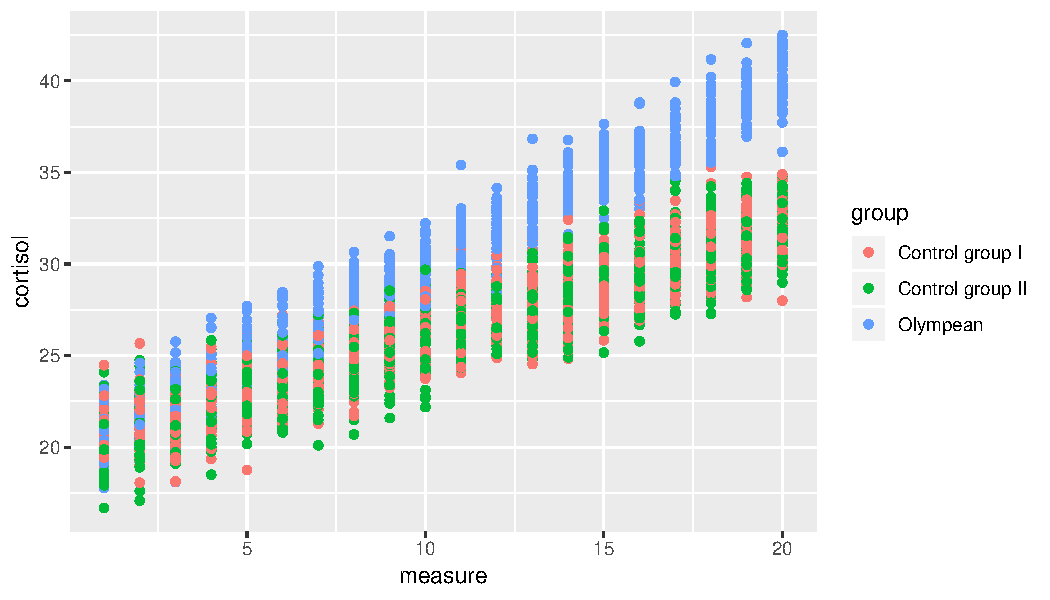
\includegraphics[width=\maxwidth]{figure/analysismixed20_2-1} 

}



\end{knitrout}

So we want to know whether the linear effect of time is moderated by group. Since for every person we have 20 measurements, the data are clustered so we use a linear mixed model. We're looking for a linear effect of time, so we use the WITH keyword to indicate that we want to use the \textbf{measure} variable in a quantitative way. We also use \textbf{group} as a predictor, but in a qualitative way, by using the keyword BY, so that SPSS will automatically make dummy variables. Because we're interested in an interaction effect, we include both main effects of \textbf{group} and \textbf{measure} and their interaction under the DESIGN subcommand. Lastly, we control for individual differences in cortisol levels by introducing a random effect for \textbf{person}.


\begin{verbatim}
MIXED cortisol WITH measure BY group 
  /FIXED=measure group measure*group
  /PRINT=DESCRIPTIVES  SOLUTION
  /RANDOM=intercept | SUBJECT(person) COVTYPE(VC).
\end{verbatim}


The SPSS output is presented below. 


\begin{figure}[h]
    \begin{center}
       \includegraphics[scale=0.8, trim={0cm 15cm 0cm 0cm}]{/Users/stephanievandenberg/Dropbox/Statistiek_Onderwijs/Data" "Analysis/spss" "examples" "linear" "mixed" "model/mixedprepost/mixed20.pdf}
    \end{center}
\end{figure}

In the output we see an intercept of 19.7, a slope of 1.0 for the effect of measure, two main effects for the group variable (group3 is the reference group, in this case the Olympeans, see the plot above), and two effects for the interaction effect (one for control group I and one for control group II). Let's fill in the linear equation based on this output:


\begin{eqnarray}
cortisol_{ij} = 19.7 + person_i + 1 \times measure + .4  ContrG1 + \nonumber\\
      0.18 ContrG2 -.4  ContrG1 \times measure -.4  ContrG2 \times measure+   e_{ij} \nonumber\\
person_i \sim N(0, \sigma_p^2 = 0.99)\nonumber\\
e_{ij} \sim N(0, \sigma_e^2 = 1.00) \nonumber
\end{eqnarray}

We see a clear intraclass correlation of around $\frac{0.986}{0.986+0.997}= 0.5 $ so it's a good thing we've included a random effect for persons. The expected means at various time points and for various groups can be made with the use of the above equation. 

It's easier to see what linear effects we have for the three different groups. Filling in the above equation for Control group 1, we get:

\begin{eqnarray}
cortisol_{ij} &=& 19.7 + person_i + 1 \times measure + .4    -.4  \times measure +   e_{ij} \nonumber \\
               &=&  20.1 + person_i +0.6 \times measure +   e_{ij} \nonumber
\end{eqnarray}

For Control group 2 we get:

\begin{eqnarray}
cortisol_{ij} &=& 19.7 + person_i + 1 \times measure  + 0.18  - .4  \times measure+   e_{ij} \nonumber \\
        &=&   19.88 + person_i   + 0.6 \times measure    +   e_{ij}    \nonumber
\end{eqnarray}

And for the Olympeans we get:

\begin{eqnarray}
cortisol_{ij} = 19.7 + person_i + 1 \times measure  +   e_{ij} \nonumber \\
\end{eqnarray}


In these equations all intercepts are around 20. The slopes are 0.6 in both Control groups I and II, whereas the slope is 1.0 in the group of Olympean athletes. For illustration, these implied linear regression lines are depicted below:


\begin{knitrout}
\definecolor{shadecolor}{rgb}{0.969, 0.969, 0.969}\color{fgcolor}

{\centering 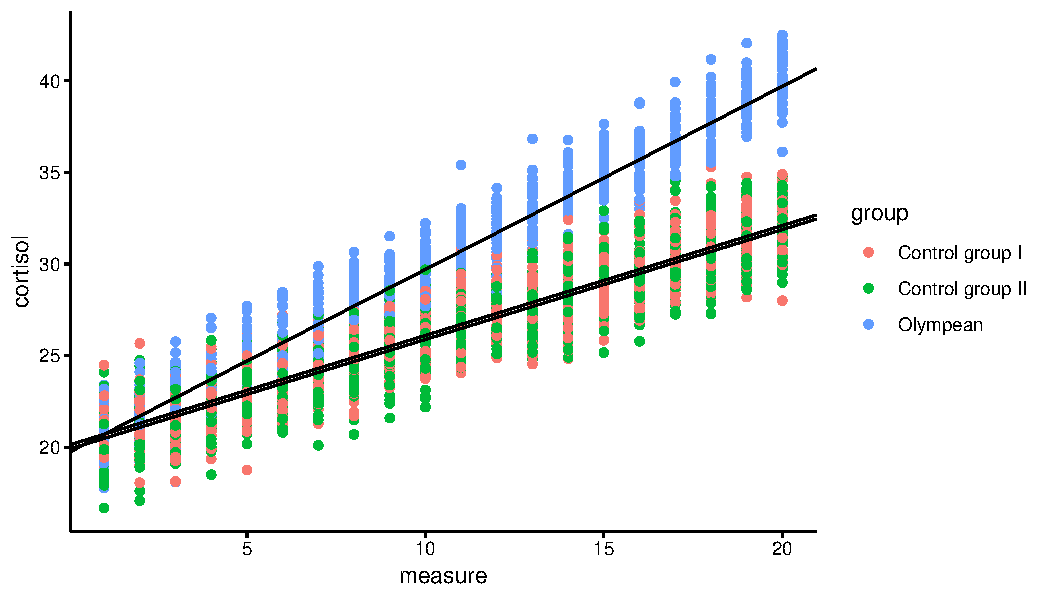
\includegraphics[width=\maxwidth]{figure/analysismixed20_3-1} 

}



\end{knitrout}

So based on the linear equation, we see that in this sample the rise in cortisol levels is much steeper in Olympeans than in the two control groups. But is this true for all Olympeans and the rest of the populations of high performing athletes and spectators? Note that in the regression table we see two interaction effects: one for \textbf{group1*measure} and one for \textbf{group2*measure}. Here we're interested in the overall signficance of the interaction effects. That answer we find in the top table with the $F$-statistics: we see a significant group by measure interaction effect, $F(2, 28)= 18.57, p<0.001$. The null-hypothesis of the same cortisol change in three different populations can be rejected, and we conclude that Olympean athletes, non-Olympean athletes and spectators show a different change in cortisol levels in the weeks preceding the games.  



 % introduction linear mixed models



\chapter{Non-parametric alternatives for linear mixed models}


\section{Checking assumptions}

In previous chapters we have discussed the assumptions of linear models and linear mixed models: linearity (in parameters), homoscedasticity (equal variance), normal distribution of residuals, normal distribution of random effects (relevant for linear mixed models only), and independence (no clustering unaccounted for). 




The problem of nonlinearity can be solved by introducing quadratic terms, for instance by replacing a linear model $Y = b_0 + b_1 X + e$ by another linear model $Y = b_0 + b_1 X + b_2 X^2 + e$.

If we have nonindependence, then you can introduce either an extra fixed effect or a random effect for this clustering. For example, if you see that cars owned by low income families have much more mileage than cars owned by high income families, you can account for this by adding a fixed effect of an income variable as predictor. If you see that average milage is rather similar within municipality but that average mileage can vary quite a lot across municipalities, you can introduce a random effect for municipality (if you have data say from 30 different municipalities). 

Unequal variance of residuals and nonnormal distribution of residuals are harder to tackle. Unequal variance can be tackled sometimes by using linear models, but with more advanced options, or by making corrections to $p$-values that make inference more robust against model violations. Violations of normality are even a bigger problem. Nonnormality can sometimes be solved by using generalized linear models (see next chapter). A combination of nonnormality and unequal variance can sometimes be solved by using a transformation of the data, for instance not analyzing $Y = b_0 + b_1 X + e$ but analyzing $log(Y)=  b_0 + b_1 X + e$ or $\sqrt{Y}=  b_0 + b_1 X + e$.

If these data transformations or advanced options don't work (or if you're not acquainted with them), and your data show nonequal variance and/or nonnormally distributed residuals, there are nonparametric alternatives.  Here we discuss two: Friedman's test and Wilcoxon's signed rank test. We explain them using an imaginary data set on speedskating.
\\
\\
Suppose we have data on 12 speedskaters that participate on the 10 kilometers distance in three separate championships in 2017-2018: the European Championships, the Winter Olympics and the World Championships. Your friend expects that speedskaters will perform best at the Olympic games, so there she expects the fastest times. So you decide to test the null-hypothesis that average times are the same at the three occasions. In Figure \ref{fig:nonparmixed_1} we see a boxplot of the data.

% H_0: $\mu_{EC}=\mu_{WC}_\mu{WO}$


\begin{knitrout}
\definecolor{shadecolor}{rgb}{0.969, 0.969, 0.969}\color{fgcolor}\begin{figure}

{\centering 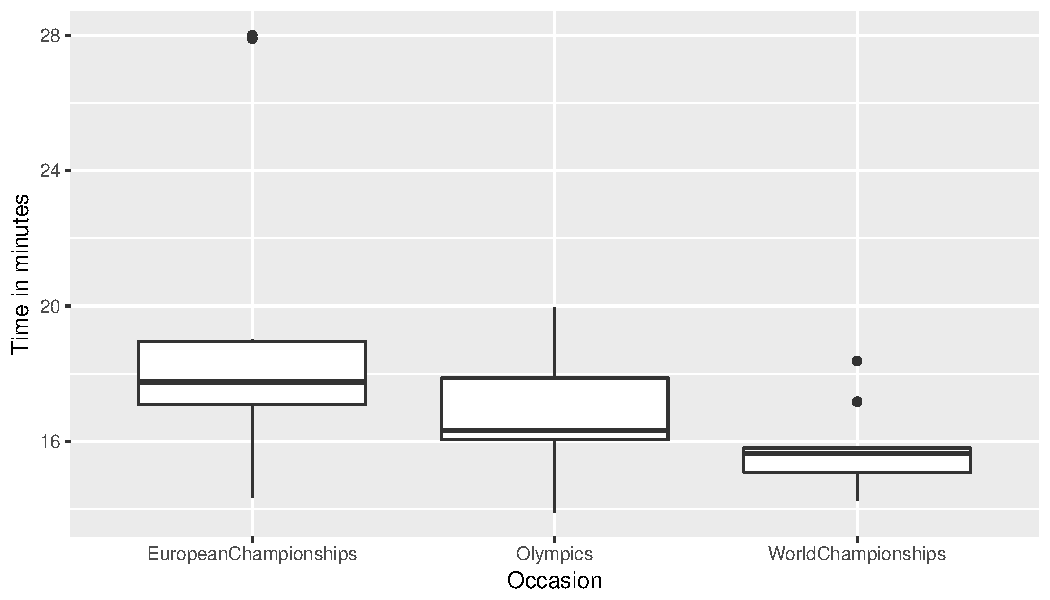
\includegraphics[width=\maxwidth]{figure/nonparmixed_1-1} 

}

\caption[Boxplot of the imaginary speed skating data]{Boxplot of the imaginary speed skating data.}\label{fig:nonparmixed_1}
\end{figure}


\end{knitrout}

In order to test this null-hypothesis, we run a linear mixed model with dependent variable time, and independent variable occasion. We use random effects for the differences in speed across skaters. In Figure \ref{fig:nonparmixed_2} we see the residuals:

\begin{knitrout}
\definecolor{shadecolor}{rgb}{0.969, 0.969, 0.969}\color{fgcolor}\begin{figure}

{\centering 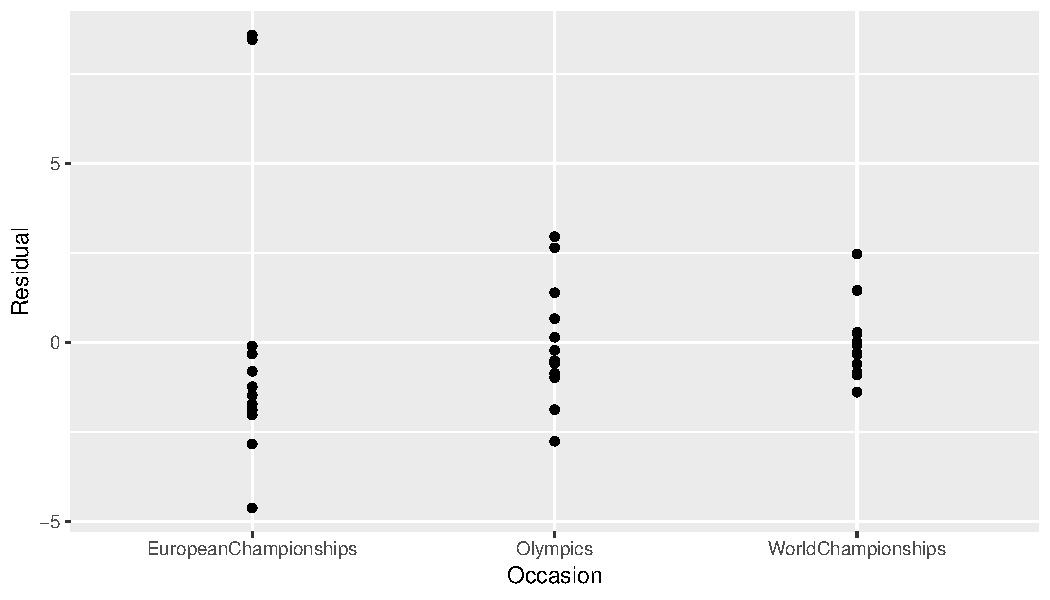
\includegraphics[width=\maxwidth]{figure/nonparmixed_2-1} 

}

\caption[Residuals of the speedskating data with a linear mixed model]{Residuals of the speedskating data with a linear mixed model.}\label{fig:nonparmixed_2}
\end{figure}


\end{knitrout}

From this plot we clearly see that the assumption of equal variance (homogeneity of variance) is violated: the variance of the residuals in the Worldchampionships condition is clearly smaller than the variance of the European championships condition. From the histogram of the residuals in Figure \ref{fig:nonparmixed_3} we also see that the distribution of the residuals is not bell-shaped: it is positively skewed (skewed to the right).




\begin{knitrout}
\definecolor{shadecolor}{rgb}{0.969, 0.969, 0.969}\color{fgcolor}\begin{figure}

{\centering 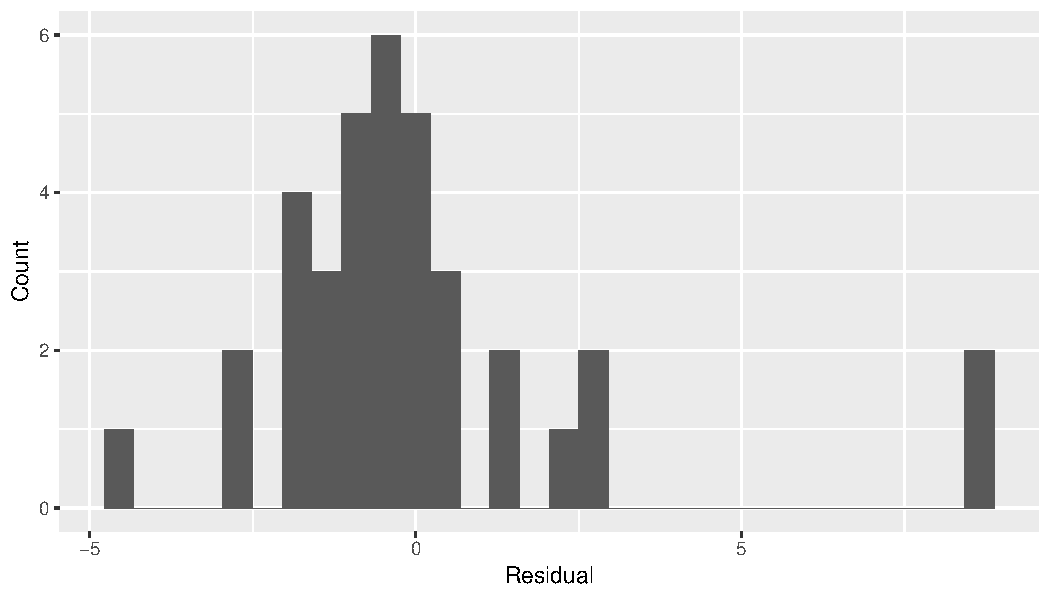
\includegraphics[width=\maxwidth]{figure/nonparmixed_3-1} 

}

\caption[Histogram of the residuals of the speedskating data with a linear mixed model]{Histogram of the residuals of the speedskating data with a linear mixed model.}\label{fig:nonparmixed_3}
\end{figure}


\end{knitrout}
% \\
% \\
Since the assumptions of homogeneity of variance and of normally distributed residuals are violated\footnote{Remember that assumptions relate to the population not samples: oftentimes your data set is too small to say anything about assumptions at the populationlevel. Residuals for a data set of 8 persons might show very nonnormal residuals, or very different variances for two subgroups of 4 persons each, but that might just be a coincidence, a random result because of the small sample size. If in doubt, it is best to use nonparametric methods.}, the results from the linear mixed model cannot be trusted. In order to answer our research question, we therefore have to resort to another kind of test. Here we discuss Friedman's test, a non-parametric test, for testing the null-hypothesis that the \textit{medians} of the three groups of data are the same. This Friedman test can be used in all situations where you have at least 2 levels of the within variable. In other words, you can use this test when you have data from three occasions, but also when you have data from 10 occassions or only 2. In the following section the Wilcoxon signed ranks test is discussed. This test is often used in social and behavioural sciences. The downside of this test is that it can only handle data sets with 2 levels of the within variable. In other words, it can only be used when we have data from two occassions. Friedman's test is therefore more generally applicable than Wilcoxon's. We therefore advise to always go with the Friedman test, but for the sake of completeness, we will also explain the Wilcoxon test.





\section{Friedman's test for $k$ measures}


Similar to many other nonparametric tests for testing the equality of medians, Friedman's test is based on ranks. Figure \ref{fig:nonparmixed_4} shows the speedskating data in wide format.


% latex table generated in R 3.4.2 by xtable 1.8-2 package
% Thu Mar  1 17:46:02 2018
\begin{table}[ht]
\centering
\caption{The speedskating data in wide format.} 
\label{tab:nonparmixed_4}
\begin{tabular}{lrrr}
  \hline
athlete & EuropeanChampionships & Olympics & WorldChampionships \\ 
  \hline
1 & 14.35 & 16.42 & 15.79 \\ 
  2 & 17.36 & 18.13 & 14.26 \\ 
  3 & 19.01 & 19.95 & 18.37 \\ 
  4 & 27.90 & 17.78 & 15.12 \\ 
  5 & 17.67 & 16.96 & 17.17 \\ 
  6 & 17.83 & 16.15 & 15.30 \\ 
  7 & 16.30 & 19.44 & 15.63 \\ 
  8 & 28.00 & 16.23 & 15.69 \\ 
  9 & 18.27 & 15.76 & 15.65 \\ 
  10 & 17.00 & 16.18 & 14.99 \\ 
  11 & 17.10 & 13.89 & 15.83 \\ 
  12 & 18.94 & 14.83 & 14.77 \\ 
   \hline
\end{tabular}
\end{table}


We rank all of these time measures by determining the fastest time, then the next to fastest time, etcetera, until the slowest time. But because the data in each row belong together (we compare individuals with themselves), we do the ranking \textit{row-wise}. For each athlete separately, we determine the fastest time (1), the next fastest time (2), and the slowest time (3) and put the ranks in a table.


% latex table generated in R 3.4.2 by xtable 1.8-2 package
% Thu Mar  1 17:46:03 2018
\begin{table}[ht]
\centering
\caption{Row-wise ranks of the speedskating data.} 
\label{tab:nonparmixed_5}
\begin{tabular}{lrrr}
  \hline
athlete & EuropeanChampionships & Olympics & WorldChampionships \\ 
  \hline
1 & 1.00 & 3.00 & 2.00 \\ 
  2 & 2.00 & 3.00 & 1.00 \\ 
  3 & 2.00 & 3.00 & 1.00 \\ 
  4 & 3.00 & 2.00 & 1.00 \\ 
  5 & 3.00 & 1.00 & 2.00 \\ 
  6 & 3.00 & 2.00 & 1.00 \\ 
  7 & 2.00 & 3.00 & 1.00 \\ 
  8 & 3.00 & 2.00 & 1.00 \\ 
  9 & 3.00 & 2.00 & 1.00 \\ 
  10 & 3.00 & 2.00 & 1.00 \\ 
  11 & 3.00 & 1.00 & 2.00 \\ 
  12 & 3.00 & 2.00 & 1.00 \\ 
   \hline
\end{tabular}
\end{table}


From this table we see for example that athlete 1 had the fastest time on the European Championships (14.35, rank 1) and the slowest at the Olympics (16.42, rank 3).


Next we compute the sum of the ranks column-wise: the sum of the ranks for the European Championships data is 31, for the Olympic data it's 26 and for the World Championships data it is 15.

From these sums we can gather that in general, these athletes showed their best times (many rank 1s) at the World Championships, as the sum of the ranks is lowest. We also see that in general these athletes showed their worst times (many rank 2s and 3s) at the European Championships, as the relevant column showed the highest sum of ranks.

In order to know whether these sums of ranks are significantly different from eachother, we may compute an $F_r$-value based on the following formula:


\begin{equation}
F_r = \left[  \frac{12}{Nk(k+1)} \Sigma^k_{j=1} S_j^2      \right] - 3N (k+1)
\end{equation}


In this formula, $N$ stands for the number of rows (12 athletes), $k$ stands for the number of columns (3 occasions), and $S_j^2$ stands for the squared sum of column $j$ ($31^2$, $26^2$ and $15^2$). If we fill in these numbers, we get:

\begin{eqnarray}
F_r &=& \left[  \frac{12}{12 \times  3(3+1)} \times (31^2 + 26^2 + 15^2)      \right] - 3 \times 12 (3+1) \nonumber \\
  &=&   \left[  \frac{12}{144} \times  1862      \right] - 144 = 11.17  \nonumber
\end{eqnarray}



What can we tell from this $F_r$-statistic? In order to say something about significance, we have to know what values are to be expected under the null-hypothesis that there are no differences across the three groups of data. Suppose we randomly mixed up the data by taking all the speedskating times and randomly assigning them to the three contests and the twelve athletes, until we have a newly filled datamatrix in Table \ref{tab:nonparmixed_26}:

% latex table generated in R 3.4.2 by xtable 1.8-2 package
% Thu Mar  1 17:46:03 2018
\begin{table}[ht]
\centering
\caption{The raw skating data in random order.} 
\label{tab:nonparmixed_26}
\begin{tabular}{lrrr}
  \hline
athlete & EuropeanChampionships & Olympics & WorldChampionships \\ 
  \hline
1 & 18.37 & 15.79 & 17.83 \\ 
  2 & 15.12 & 14.83 & 17.67 \\ 
  3 & 14.35 & 14.99 & 15.63 \\ 
  4 & 14.26 & 17.00 & 17.36 \\ 
  5 & 19.01 & 16.30 & 17.17 \\ 
  6 & 16.23 & 15.30 & 14.77 \\ 
  7 & 15.83 & 15.69 & 27.90 \\ 
  8 & 15.76 & 19.44 & 13.89 \\ 
  9 & 15.65 & 18.27 & 16.18 \\ 
  10 & 28.00 & 17.78 & 16.15 \\ 
  11 & 19.95 & 16.42 & 17.10 \\ 
  12 & 18.13 & 16.96 & 18.94 \\ 
   \hline
\end{tabular}
\end{table}


If we then compute $F_r$ for these mixed up data, we get another value. If we do this say 1000 times, we get the following values for $F_r$, summarized in the  histogram in Figure \ref{fig:nonparmixed_36}.

%fig.cap='Histogram of 1000 possible values for F_r given that the null-hypothesis is true, for 12 speedskaters.'

\begin{knitrout}
\definecolor{shadecolor}{rgb}{0.969, 0.969, 0.969}\color{fgcolor}\begin{figure}

{\centering 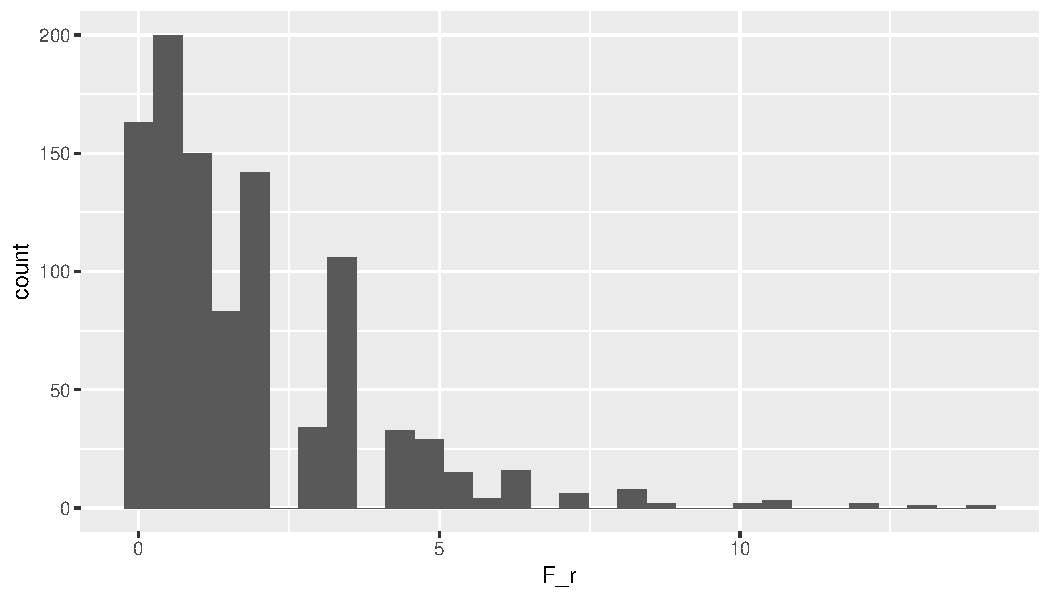
\includegraphics[width=\maxwidth]{figure/nonparmixed_36-1} 

}

\caption[Histogram of 1000 possible values for Fr given that the null-hypothesis is true, for 12 speedskaters]{Histogram of 1000 possible values for Fr given that the null-hypothesis is true, for 12 speedskaters.}\label{fig:nonparmixed_36}
\end{figure}


\end{knitrout}

So if the data is just randomly distributed over the three columns in the data matrix, we expect no systematic differences and so the null-hypothesis is true. So now we know what the distribution of $F_r$ looks like when the null-hypothesis is true. Remember that for the true data that we actually gathered, we found an $F_r$-value of 11.17. From the histogram, we see that only very few values of 11.17 or larger are observed when the null-hypothesis is true. If we look more closely, we find that only 0.4\% of the values are larger than 11.17, so we have a $p$-value of 0.004. The 95th percentile of these 1000 $F_r$-values is 5.1666667, meaning that of the 1000 values for $F_r$, 5\% are larger than 5.1666667. So if we use a signficance level of 5\%, our observed value of 11.17 is larger than the critical value for $F_r$, and we conclude that the null-hypothesis can be rejected.

Now this $p$-value of 0.004 and the critical value of 5.1666667 are based on our own computations. Actually there are better ways. One is to look up critical values of $F_r$ in tables, for instance in Kendall M.G. (1970) \textit{Rank correlation methods}. (fourth edition). The $p$-value corresponding to this $F_r$-value depends on $k$, the number of groups of data (here 3 columns) and $N$, the number of rows (12 individuals). If we look up that table, we find that for $k=3$ and $N=12$ the critical value of $F_r$ for a type I error rate of 0.05 equals 6.17. Our observed $F_r$-value of 11.17 is larger than that, therefore we can reject the null-hypothesis that the median skating times are the same at the three different championships. So we have to tell your friend that there are general differences in skating times at different contests, $F_r=11.17, p < 0.05$, but it is not the case that the fastest times were observed at the Olympics.

Another way is to make an approximation of the distribution of $F_r$. Note that the distribution in the histogram is very strangely shaped. The reason is that the data set is quite limited. Suppose we have not data on 12 speedskaters, but on 120. If we then randomly mix up data again and compute 1000 different values for $F_r$, we get the histogram in Figure \ref{fig:nonparmixed_46}.


\begin{knitrout}
\definecolor{shadecolor}{rgb}{0.969, 0.969, 0.969}\color{fgcolor}\begin{figure}

{\centering 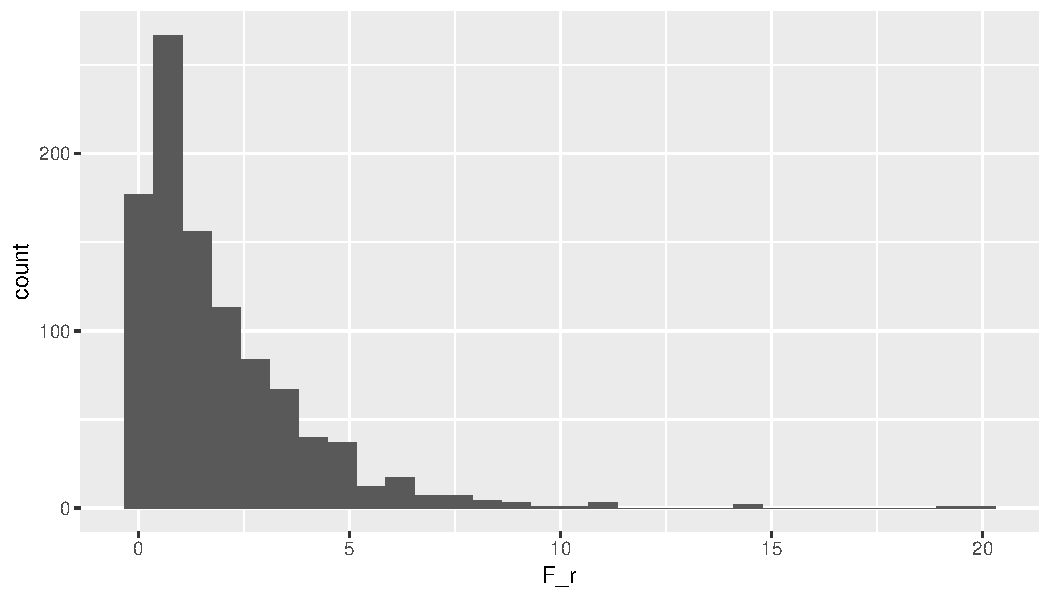
\includegraphics[width=\maxwidth]{figure/nonparmixed_46-1} 

}

\caption[Histogram of 1000 possible values for Fr given that the null-hypothesis is true, for 120 speedskaters]{Histogram of 1000 possible values for Fr given that the null-hypothesis is true, for 120 speedskaters.}\label{fig:nonparmixed_46}
\end{figure}


\end{knitrout}

The shape becomes more regular. It also starts to resemble another distribution, that of the $\chi^2$ (chi-square). It can be shown that the distribution of the $F_r$ for a large number of rows in the data matrix, and at least 6 columns, approaches the shape of the $\chi^2$-distribution with $k-1$ degrees of freedom. This is shown in Figure \ref{fig:nonparmixed_56}.

\begin{knitrout}
\definecolor{shadecolor}{rgb}{0.969, 0.969, 0.969}\color{fgcolor}\begin{figure}

{\centering \includegraphics[width=\maxwidth]{figure/nonparmixed_56-1} 

}

\caption[The distrbution of Fr under the null-hypothesis, overlain with a chi-square distribution with 2 degrees of freedom]{The distrbution of Fr under the null-hypothesis, overlain with a chi-square distribution with 2 degrees of freedom.}\label{fig:nonparmixed_56}
\end{figure}


\end{knitrout}

The line of the $\chi^2$-distribution with 2 degrees of freedom approaches the histogram quite well, but not perfectly. In general, for large $N$ and $k>5$, the approximation is good enough. In that way it gets easier to look up $p$-values for certain $F_r$-values, because the $\chi^2$-distribution is well-known\footnote{The $\chi^2$-distribution is based on the normal distribution: the $\chi^2$-distribution with $k$ degrees of freedom is the distribution of a sum of the squares of $k$ independent standard normal random variables.}, so we don't have to look up critical values for $F_r$ in old tables. For a significance level of 5\%, the critical value of a $\chi^2$ with 2 degrees of freedom is 5.991. This is close to the value in the table for $F_r$ in old books: 6.17. The part of the $\chi^2$-distribution with 2 degrees of freedom that is larger than the observed 11.17 is 0.0037537, so our approximate $p$-value for our null-hypothesis is 0.004.


\section{How to perform Friedman's test in SPSS}

First of all, you need data in wide format. If your data happens to be in long format, use the CASETOVARS procedure to get the data in wide format. CASETOVARS requires your data to be ordered, so use the SORT CASE BY procedure before CASETOVARS. Suppose your data is in long format, as in Table \ref{tab:nonparmixed_6}.

% latex table generated in R 3.4.2 by xtable 1.8-2 package
% Thu Mar  1 17:46:07 2018
\begin{table}[ht]
\centering
\caption{The raw skating data in long data format.} 
\label{tab:nonparmixed_6}
\begin{tabular}{lrr}
  \hline
athlete & occasion & time \\ 
  \hline
1 & 1.00 & 14.35 \\ 
  1 & 2.00 & 16.42 \\ 
  1 & 3.00 & 15.79 \\ 
  2 & 1.00 & 17.36 \\ 
  2 & 2.00 & 18.13 \\ 
  2 & 3.00 & 14.26 \\ 
   \hline
\end{tabular}
\end{table}



Then the following syntax turns the data into wide format:


\begin{verbatim}
SORT CASES BY athlete occasion.
CASESTOVARS
  /ID=athlete
  /INDEX=occasion
  /GROUPBY=VARIABLE
 /SEPARATOR = "_".
\end{verbatim}


This creates the wide format data matrix in Table \ref{tab:nonparmixed_7}:


% latex table generated in R 3.4.2 by xtable 1.8-2 package
% Thu Mar  1 17:46:07 2018
\begin{table}[ht]
\centering
\caption{The raw skating data in wide data format after CASETOVARS} 
\label{tab:nonparmixed_7}
\begin{tabular}{lrrr}
  \hline
athlete & time\_1.00 & time\_2.00 & time\_3.00 \\ 
  \hline
1 & 14.35 & 16.42 & 15.79 \\ 
  2 & 17.36 & 18.13 & 14.26 \\ 
  3 & 19.01 & 19.95 & 18.37 \\ 
  4 & 27.90 & 17.78 & 15.12 \\ 
  5 & 17.67 & 16.96 & 17.17 \\ 
  6 & 17.83 & 16.15 & 15.30 \\ 
  7 & 16.30 & 19.44 & 15.63 \\ 
  8 & 28.00 & 16.23 & 15.69 \\ 
  9 & 18.27 & 15.76 & 15.65 \\ 
  10 & 17.00 & 16.18 & 14.99 \\ 
  11 & 17.10 & 13.89 & 15.83 \\ 
  12 & 18.94 & 14.83 & 14.77 \\ 
   \hline
\end{tabular}
\end{table}


Note the variable names: they start with the dependent variable time and are then indexed by the number of the occasion, 1.00, 2.00 and 3.00, that relate to European Championships, Olympic Games and World Championships, respectively.

We can then specify that we want Friedman's test by using the NPAR TESTS procedure with the FRIEDMAN subcommand and indicating which variables we want to use:

\begin{verbatim}
NPAR TESTS
/FRIEDMAN=time_1.00 time_2.00 time_3.00.
\end{verbatim}

\begin{figure}[h]
    \begin{center}
       \includegraphics[scale=0.8, trim={0cm 22cm 0cm 0cm}]{/Users/stephanievandenberg/Dropbox/Statistiek_Onderwijs/Data" "Analysis/spss" "examples" "nonparmixed/friedman1.pdf}
    \end{center}
     \caption{SPSS output of the Friedman test.}
    \label{fig:friedman1}
\end{figure}


In the output in Figure \ref{fig:friedman1} you first see the mean ranks. Note that if you multiply these by 12 (the number of rows), you get the sum of the ranks per column that we also computed above. Next you see a chi-square statistic, degrees of freedom, and an asymptotic $p$-value (Asymp. Sig.). Why don't we see an $F_r$-statistic?

The reason is, as discussed in the previous section, that for large number of measurements (columns) and a large number of individuals (rows), the $F_r$ statistic tends to behave like a chi-square, $\chi^2$, with $k-1$ degrees of freedom. So what we are looking at in this output is really an $F_r$-value of 11.17 (exactly the same value as we computed by hand in the previous section). In order to approximate the $p$-value, this value of 11.17 is interpreted as a chi-square ($\chi^2$), which with 2 degrees of freedom has a $p$-value of 0.004.


This asymptotic (approximated) $p$-value is the correct $p$-value if you have a lot of rows (large $N$) and at least 6 variables ($k>5$). If you do not have that, as we have here, this asymptotic $p$-value is only what it is: an approximation. If you want to have the exact $p$-value, then do

\begin{verbatim}
NPAR TESTS
/FRIEDMAN=time_1.00 time_2.00 time_3.00
/METHOD=EXACT.
\end{verbatim}

and then use the $p$-value under $exact sign.$, in this case 0.002, see Figure \ref{fig:friedman2}.

\begin{figure}[h]
    \begin{center}
       \includegraphics[scale=0.8, trim={0cm 22cm 0cm 0cm}]{/Users/stephanievandenberg/Dropbox/Statistiek_Onderwijs/Data" "Analysis/spss" "examples" "nonparmixed/friedman2.pdf}
    \end{center}
    \caption{SPSS output of the Friedman test with the exact p-value.}
    \label{fig:friedman2}
\end{figure}


Thus, a Friedman's test of equal medians showed that speedskaters show significantly different median times on the 10 kilometer distance at the three types of contests, $F_r=11.17, p=0.002$.



\section{Wilcoxon's signed ranks test for 2 measures}

Friedman's test can be used for 2 measures, 3 measures or even 10 measures. As stated earlier, the well-known Wilcoxon's test can only be used for 2 measures. For completeness, we also discuss that test here.
\\
\\
For each athlete, we take the difference in skating times and call it $d$, see Table \ref{tab:nonparmixed_77}. Next we rank these $d$-values, irrespective of sign, and call these ranks $rank_d$. From the table \ref{nonparmixed_77} we see that athlete 12 shows the smallest difference in skating times ($d$= 0.06, rank = 1) and athlete 2 the largest difference.

% latex table generated in R 3.4.2 by xtable 1.8-2 package
% Thu Mar  1 17:46:07 2018
\begin{table}[ht]
\centering
\caption{The raw skating data and the computations for Wilcoxon signed ranks test} 
\label{tab:nonparmixed_77}
\begin{tabular}{lrrrrr}
  \hline
athlete & Olympics & WorldChampionships & d & rank\_d & ranksign \\ 
  \hline
1 & 16.42 & 15.79 & 0.63 & 5.00 & 5.00 \\ 
  2 & 18.13 & 14.26 & 3.87 & 12.00 & 12.00 \\ 
  3 & 19.95 & 18.37 & 1.58 & 8.00 & 8.00 \\ 
  4 & 17.78 & 15.12 & 2.66 & 10.00 & 10.00 \\ 
  5 & 16.96 & 17.17 & -0.21 & 3.00 & -3.00 \\ 
  6 & 16.15 & 15.30 & 0.85 & 6.00 & 6.00 \\ 
  7 & 19.44 & 15.63 & 3.81 & 11.00 & 11.00 \\ 
  8 & 16.23 & 15.69 & 0.54 & 4.00 & 4.00 \\ 
  9 & 15.76 & 15.65 & 0.11 & 2.00 & 2.00 \\ 
  10 & 16.18 & 14.99 & 1.19 & 7.00 & 7.00 \\ 
  11 & 13.89 & 15.83 & -1.94 & 9.00 & -9.00 \\ 
  12 & 14.83 & 14.77 & 0.06 & 1.00 & 1.00 \\ 
   \hline
\end{tabular}
\end{table}


Next we indicate for each rank whether it belongs to a positive or a negative difference $d$ and call that variable \textbf{ranksign}.

Under the null-hypothesis, we expect that some of the larger $d$-values are positive and some of them negative, in a fairly equal amount. If we sum the ranks having plus-signs and sum the ranks having minus-signs, we would expect that these two sums are about equal, but only if the null-hypothesis is true. If the sums are very different, then we should reject this null-hypothesis. In order to see if the difference in sums is too large, we compute them as follows:


\begin{eqnarray}
T^+ &=& 5+ 12 + 8 +10+6+11+4 +2 +7 +1 = 66 \nonumber \\
T^- &=& 3 + 9= 12 \nonumber
\end{eqnarray}



To know whether $T^+$ is significantly larger than $T^-$, the value of $T^+$ can be looked up in a table, for instance in Siegel \& Castellan (1988). There we see that for $T^+$, with 12 rows, the probability of obtaining a $T^+$ of at least 66 is 0.0171. For a two-sided test (if we would have switched the columns of the two championships, we would have gotten a $T^-$ of 66 and a $T^+$ of 12!), we have to double this probability. So we end up with a $p$-value of $2 \times 0.0171=0.0342$.


In the table we find no critical values for large sample size $N$, but fortunately, similar to the Friedman test, we use an approximation using the normal distribution. It can be shown that for large sample sizes, the statistic $T^+$ is approximately normally distributed with mean


\begin{equation}
\mu = \frac{N(N+1)}{4}
\end{equation}

and variance:

\begin{equation}
\sigma^2= \frac {N(N+1)(2N+1)  }  {24}
\end{equation}


If we therefore standardize the $T^+$ by subtracting the $\mu$ and then dividing by the square root of the variance $\sqrt(\sigma^2)=\sigma$, we get a $Z$-value with mean 0 and standard deviation 1. To do that, we use the following formula:

\begin{equation}
Z = \frac{T^+ - \mu}{\sigma} =  \frac  { T^+ - N(N+1)/4} {\sqrt{N(N+1)(2N+1)/24}}
\end{equation}


Here $T^+$ is 66 and $N$ equals 12, so if we fill in the formula we get $Z= 2.1180543$. From the standard normal distribution we know that 5\% of the observations lie above 1.96 and below -1.96. So a value for $Z$ larger than 1.96 or smaller than -1.96 is enough evidence to reject the null-hypothesis. Here our $Z$-statistic is larger than 1.96, therefore we reject the null-hypothesis that the median skating times are the same at the World Championships and the Olympics. The $p$-value associated with a $Z$-score of 2.1180543 is 0.034.





\section{How to perform Wilcoxon's signed ranks test in SPSS}

If you want to use the Wilcoxon test, then use the following syntax:

\begin{verbatim}
NPAR TESTS
/WILCOXON=time_2.00 time_3.00
/METHOD=EXACT.
\end{verbatim}


\begin{figure}[h]
    \begin{center}
       \includegraphics[scale=0.8, trim={0cm 18cm 0cm 0cm}]{/Users/stephanievandenberg/Dropbox/Statistiek_Onderwijs/Data" "Analysis/spss" "examples" "nonparmixed/wilcoxon1.pdf}
    \end{center}
    \caption{SPSS output of the Wilcoxon test.}
    \label{fig:wilcoxon1}
\end{figure}

In the output in Figure \ref{fig:wilcoxon1} we see a $Z$-statistic, an asymptotic $p$-value, and two exact $p$-values. The reason that we see a $Z$-statistic is that the Wilcoxon $T^+$ statistic approaches a normal distribution in case we have a large number of observations (many rows). If $N>15$, the approximation is good enough so that the statistic can be interpreted as a $z$-score (standardized score with a normal distribution). That means that a $z$-score of 1.96 or larger or -1.96 or smaller can be regarded as significant at the 5\% significance level. Since the standard normal distribution is only an approximation, and we have $N=12$, we have to look at the exact significance level, which is in this case 0.034. We see that the exact $p$-value is in this case equal to the approximate $p$-value. Note that we use a two-sided test, to allow for the fact that random sampling could lead to a higher median for the Olympic Games or a higher median for the World Championships. We just want to know whether the null-hypothesis that the two medians differ can be rejected (in whatever direction) or not.
\\
\\


Let's compare the output with the Friedman test, but then only use the relevant variables in your syntax:

\begin{verbatim}
NPAR TESTS
/FRIEDMAN=  time_2.00 time_3.00
/METHOD=EXACT.
\end{verbatim}


In the output in Figure \ref{fig:friedman3} we see that the null-hypothesis of equal medians at the World Championships and the Olympic Games can be rejected, with a $p$-value of 0.039.

\begin{figure}[h]
    \begin{center}
       \includegraphics[scale=0.8, trim={0cm 22cm 0cm 0cm}]{/Users/stephanievandenberg/Dropbox/Statistiek_Onderwijs/Data" "Analysis/spss" "examples" "nonparmixed/friedman3.pdf}
    \end{center}
    \caption{SPSS output of the Friedman test for two measures.}
    \label{fig:friedman3}
\end{figure}



Note that both the Friedman and Wilcoxon tests come up with very similar $p$-values. Their rationales are very similar: Friedman's test is based on ranks and Wilcoxon's test is based on positive and negative differences between measures 1 and 2, so in fact ranks 1 and 2 for each row in the data matrix. Both can therefore be used in the case you have two measures. We recommend to use the Friedman test, since that test can be used in all situations where you have 2 or more measures per row. Wilcoxon's test can only be used if you have 2 measures per row.
\\
\\
In sum, we can report in two ways on our hypothesis regarding similar skating times at the World Championships and at the Olympics:

\begin{enumerate}

\item

\begin{quotation}
A Friedman test showed a significant difference between the 10km skating times at the World Championships and at the Olympics, $F_r = 5.33, p=0.04$. Athletes more often show their fastest times at the World Championships than can be expected due to chance.
\end{quotation}

\item

\begin{quotation}
A Wilcoxon signed ranks test showed a significant difference between the 10km skating times at the World Championships and at the Olympics, $Z = -2.12, p=0.03$. Athletes more often show their fastest times at the World Championships than can be expected due to chance.
\end{quotation}

\end{enumerate}

How do we know that the fastest times were at the World Championships? If we look at raw data above, that does not seem that obvious. But this conlusion is based on the sum of ranks: we saw a sum of ranks of 26 for the Olympics and 15 for the World Championships. So the average rank is lower at the World Championships.


\section{Ties}

Many nonparametric tests are based on ranks. For example, if we have the data sequence {0.1, 0.4, 0.5, 0.2}, we give these values the ranks {1, 3, 4, 2}, respectively. But in may data cases, data sequences cannot be ranked unequivocally. Let's look at the sequence {0.1, 0.4, 0.4, 0.2}. Here we have 2 values that are exactly the same. We say then that we have \textit{ties}. If we have ties in our data like the 0.4 in this case, one very often used option is to arbitrarily choose one of the 0.4 values as smaller than the other, and then average the ranks. Thus, we rank the data into {1, 3, 4, 2} and then average the tied observations: {1, 3.5, 3.5, 2}. As another example, suppose we have the sequence {23, 54, 54, 54, 19}, we turn this into ranks {2, 3, 4, 5, 1} and take the average of the ranks of the tied observations of 54: {2, 4, 4, 4, 1}. These ranks corrected for ties can then be used to compute the test statistic, for instance Friedman's $F_r$ or Wilcoxon's $Z$. However, in many cases, because of these corrections, a slightly different formula is to be used. So the formulas become a little bit different. This is all done in SPSS automatically. If you want to know more, see Siegel and Castellan (1988).




\section{Exercises}


A researcher is interested in the relationship between mood and day of the week: are people generally moodier on Monday than on Wednesday or Friday?

Below we see the data on 4 people that rated their mood from 1 (very moody) to 10 (not moody at all) on three separate days in a week in February: Day 1 is Monday, day 2 is Wednesday and day 3 is Friday:

\begin{knitrout}
\definecolor{shadecolor}{rgb}{0.969, 0.969, 0.969}\color{fgcolor}
\begin{tabular}{r|r|r}
\hline
ID & Day & Mood\\
\hline
1 & 1 & 3\\
\hline
1 & 2 & 5\\
\hline
1 & 3 & 8\\
\hline
2 & 1 & 4\\
\hline
2 & 2 & 7\\
\hline
2 & 3 & 6\\
\hline
3 & 1 & 2\\
\hline
3 & 2 & 4\\
\hline
3 & 3 & 1\\
\hline
4 & 1 & 9\\
\hline
4 & 2 & 5\\
\hline
4 & 3 & 3\\
\hline
\end{tabular}


\end{knitrout}

\begin{enumerate}

\item Put the data into wide format, and think of appropriate variable names
\\
 \\
 \begin{tabular}{llrrrr}
   & \dots & \dots  & \dots & \dots  & \dots  \\ \hline
  & \dots & \dots  & \dots & \dots  & \dots  \\
  & \dots & \dots  & \dots & \dots  & \dots  \\
  & \dots & \dots  & \dots & \dots  & \dots  \\
  & \dots & \dots  & \dots & \dots  & \dots  \\
  & \dots & \dots  & \dots & \dots  & \dots  \\
  & \dots & \dots  & \dots & \dots  & \dots  \\
  & \dots & \dots  & \dots & \dots  & \dots  \\
  & \dots & \dots  & \dots & \dots  & \dots  \\
  & \dots & \dots  & \dots & \dots  & \dots  \\
  & \dots & \dots  & \dots & \dots  & \dots  \\
  & \dots & \dots  & \dots & \dots  & \dots  \\
  & \dots & \dots  & \dots & \dots  & \dots  \\
 \end{tabular}
\\
\\
\item Rank these data row-wise: for each row determine the lowest mood (1), the second lowest mood (2) and the highest mood score (3)
\\
 \\
 \begin{tabular}{llrrrr}
   & \dots & \dots  & \dots & \dots  & \dots  \\ \hline
  & \dots & \dots  & \dots & \dots  & \dots  \\
  & \dots & \dots  & \dots & \dots  & \dots  \\
  & \dots & \dots  & \dots & \dots  & \dots  \\
  & \dots & \dots  & \dots & \dots  & \dots  \\
  & \dots & \dots  & \dots & \dots  & \dots  \\
  & \dots & \dots  & \dots & \dots  & \dots  \\
  & \dots & \dots  & \dots & \dots  & \dots  \\
  & \dots & \dots  & \dots & \dots  & \dots  \\
  & \dots & \dots  & \dots & \dots  & \dots  \\
  & \dots & \dots  & \dots & \dots  & \dots  \\
  & \dots & \dots  & \dots & \dots  & \dots  \\
  & \dots & \dots  & \dots & \dots  & \dots  \\
 \end{tabular}
\\
\\
\item Determine the column sums: the sum of the ranks for Monday, Wednesday and Friday.
\item How many rows do you have ($N$) and how many columns of data do you have ($k$)?
\item Compute $F_r$.
\item Copy the data into SPSS and run a Friedman's test. Should you ask for an exact $p$-value? Provide the syntax.
\item Suppose you get the SPSS output in Figure \label{ref:friedmanmood1}. What would your conclusion be regarding the research question about the relationship between moodiness and the day of the week?

\begin{figure}[h]
    \begin{center}
       \includegraphics[scale=0.8, trim={0cm 20cm 0cm 0cm}]{/Users/stephanievandenberg/Dropbox/Statistiek_Onderwijs/Data" "Analysis/spss" "examples" "nonparmixed/friedmanmood1.pdf}
    \end{center}
    \caption{SPSS output of a Friedman test.}
    \label{fig:friedmanmood1}
\end{figure}

\item
In this data set, for which day did we observe the personal best mood? How many of the individuals showed their best mood on that day?


\item
A linear mixed model was run on this data set. When checking model assumptions, we saw the following graphs in Figures \ref{fig:nonparmixed_11a} and \ref{fig:nonparmixed_11b}.

\begin{knitrout}
\definecolor{shadecolor}{rgb}{0.969, 0.969, 0.969}\color{fgcolor}\begin{figure}

{\centering \includegraphics[width=\maxwidth]{figure/nonparmixed_11a-1} 

}

\caption[Residual plot after a linear mixed model analysis]{Residual plot after a linear mixed model analysis.}\label{fig:nonparmixed_11a1}
\end{figure}

\begin{figure}

{\centering \includegraphics[width=\maxwidth]{figure/nonparmixed_11a-2} 

}

\caption[Residual plot after a linear mixed model analysis]{Residual plot after a linear mixed model analysis.}\label{fig:nonparmixed_11a2}
\end{figure}


\end{knitrout}

\begin{knitrout}
\definecolor{shadecolor}{rgb}{0.969, 0.969, 0.969}\color{fgcolor}\begin{figure}

{\centering \includegraphics[width=\maxwidth]{figure/nonparmixed_11b-1} 

}

\caption[Histogram of residuals after a linear mixed model analysis]{Histogram of residuals after a linear mixed model analysis.}\label{fig:nonparmixed_11b}
\end{figure}


\end{knitrout}


Would you prefer to stick to the Friedman's test for this data set, or would you prefer to report a linear mixed model? Explain your answer.

\item Could you have performed a Wilcoxon test on these data? Why, or why not?

\end{enumerate}


Answers:
\begin{enumerate}

\item
The raw data in wide format:
\begin{knitrout}
\definecolor{shadecolor}{rgb}{0.969, 0.969, 0.969}\color{fgcolor}
\begin{tabular}{r|r|r|r}
\hline
ID & Mood\_1 & Mood\_2 & Mood\_3\\
\hline
1 & 3 & 5 & 8\\
\hline
2 & 4 & 7 & 6\\
\hline
3 & 2 & 4 & 1\\
\hline
4 & 9 & 5 & 3\\
\hline
\end{tabular}


\end{knitrout}

\item
The row-wise ranked data:
\begin{knitrout}
\definecolor{shadecolor}{rgb}{0.969, 0.969, 0.969}\color{fgcolor}
\begin{tabular}{r|r|r|r}
\hline
ID & Mood\_1 & Mood\_2 & Mood\_3\\
\hline
1 & 1 & 2 & 3\\
\hline
2 & 1 & 3 & 2\\
\hline
3 & 2 & 3 & 1\\
\hline
4 & 3 & 2 & 1\\
\hline
\end{tabular}


\end{knitrout}
\item Day 1: 7, Day 2: 10 and Day3: 7.
\item $N=4$ and $k=3$
\item

\begin{eqnarray}
F_r &=& \left[  \frac{12}{4 \times  3(3+1)} \times (7^2 + 10^2 + 7^2)      \right] - 3 \times 4 (3+1) \nonumber \\
  &=&   \left[  \frac{12}{48} \times  198      \right] - 48 = 1.50  \nonumber
\end{eqnarray}

\item

\begin{verbatim}
NPAR TESTS
/FRIEDMAN=  Mood_1   Mood_2    Mood_3
/METHOD=Exact.
\end{verbatim}

\item
\begin{quotation}
We found no significant effect of day of the week on mood, $F_r=1.50, p=0.65$, so the null-hypothesis of equal mood during the week is not rejected. Note however that the sample size was extremely small (12 data points), so even if there is a real relationship between mood and day of the week, there was little chance to find evidence of that in this data set.
\end{quotation}

\item The highest column sum of the ranks was found for day 2, which was Wednesday. So in this data set we saw that the four individuals generally showed their personal highest mood score on Wednesday. Actually, 2 persons out of 4 showed their highest score (rank 3) on Wednesday (ID=2 and ID=3).

\item The plots suggests that the variance of the residuals is very small for the second day, compared to the other two days. The distribution is also hardly normal. But it is hard to tell whether the assumptions are reasonable, since there are so few data points. It would therefore be safest to report a Friedman test.

\item A Wilcoxon test can only be performed on two measures, say Monday and Wednesday data, or Monday and Friday data. You could not test the null-hypothesis of the same moods on three days with a Wilcoxon test.

\end{enumerate}









\chapter{Generalized linear models}

\section{Introduction}
In previous chapters we were introduced to the linear model, with its basic form


\begin{eqnarray}
y = b_0 + b_1 X_1 + \dots + b_n X_n + e \\
e \sim N(0, \sigma_e^2)
\end{eqnarray}

The basic assumptions of this model is the linearity in the parameters, and the normally distributed residual $e$. Linearity in the parameters means that the effects of intercept and the independent variables $X_1 \dots X_n$ are additive: the assumption is that you can sum these effects to come to a predicted value for $y$. So that is also true when we include interaction effects to account for moderation effects, 

\begin{eqnarray}
y = b_0 + b_1 X_1 +  b_2 X_2 + b_3 X_1 X_2 + e \\
e \sim N(0, \sigma_e^2)
\end{eqnarray}


or when we use a quadratic term to account for other types of nonlinearity in the data:


\begin{eqnarray}
y = b_0 + b_1 X_1 +  b_2 X_1 X_1 + e \\
e \sim N(0, \sigma_e^2)
\end{eqnarray}

In all these models, the assumption is that the effects of the parameters can be added to one another. 

The other major assumption of linear (mixed) models is the normal distribution of the residuals. As we have seen in for instance the previous chapter, sometimes the residuals are not normally distributed. Remember that with a normal distribution $N(0,\sigma^2)$, in principle all values between $-\infty$ and $+\infty$ are possible, but they tend to concentrate around the value of 0, in the shape of the bell-curve. Figure \ref{fig:gen_1} shows the normal distribution $N(0,\sigma^2=4)$: it is centered around 0 and has variance 4. Note that the inflection point, that is the point where the decrease in density tends to decelerate, is exactly at the values -2 and +2. These are equal to the square root of the variance, which is the standard deviation, $+\sigma$ and $-\sigma$.


\begin{knitrout}
\definecolor{shadecolor}{rgb}{0.969, 0.969, 0.969}\color{fgcolor}\begin{figure}

{\centering \includegraphics[width=\maxwidth]{figure/gen_1-1} 

}

\caption[Density function of the normal distribution, with mean 0 and variance 4 (standard deviation 2)]{Density function of the normal distribution, with mean 0 and variance 4 (standard deviation 2). Inflection points are positioned at residual values of minus 1 standard deviation and plus 1 standard deviation.}\label{fig:gen_1}
\end{figure}


\end{knitrout}

A normal distribution is suitable for continuous data: for example a variable that can take all possible values between -1 and 0. For many data sets this is not true. Think for example of temperature measures: if the thermometer gives degrees centigrade with a precision of only 1 decimal, we can never have values of say 10.07 or -56.789. Our data will in fact be \textit{discrete}, showing rounded values like 10.1, 10.2, 10.3, but no values in between. 

Nevertheless, the normal distribution can still be used in many such cases. Take for instance a data set where the temperature in Amsterdam in summer was predicted on the basis of a linear model. Fig \ref{fig:gen_2} shows the distribution of the residuals of that model:

\begin{knitrout}
\definecolor{shadecolor}{rgb}{0.969, 0.969, 0.969}\color{fgcolor}\begin{figure}

{\centering \includegraphics[width=\maxwidth]{figure/gen_2-1} 

}

\caption[Even if residuals are really discrete, the normal distribution can be a good approximation of their distribution]{Even if residuals are really discrete, the normal distribution can be a good approximation of their distribution.}\label{fig:gen_2}
\end{figure}


\end{knitrout}


The temperature measures were discrete with a precicsion of one tenth of a degree centigrade, but the distribution seems well approximated by a normal curve. 


But let's look at an example where the discreteness is more prominent. In Figure \ref{fig:gen_3} we see the residuals of an analysis of exam results. Students had to do an asssignment that had to meet 4 criteria: 1) originality, 2) language, 3) structure, and 4) literature review. Each criterion was scored as either fulfilled (1) or not fulfilled (0). The score for the assignment was given on the basis of \textit{the number of criteria} that were met, so the scores could be 0, 1, 2, 3 or 4. The score was predicted on the basis of the average exam score on previous assignments using a linear model. 


\begin{knitrout}
\definecolor{shadecolor}{rgb}{0.969, 0.969, 0.969}\color{fgcolor}\begin{figure}

{\centering \includegraphics[width=\maxwidth]{figure/gen_3-1} 

}

\caption[Count data example where the normal distribution is not a good approximation of the distribution of the residuals]{Count data example where the normal distribution is not a good approximation of the distribution of the residuals.}\label{fig:gen_3}
\end{figure}


\end{knitrout}


Figure \ref{fig:gen_3} shows that the residuals are very discrete, and that the continous normal distribution is a very bad approximation of the histogram. We often seen this phenomenon when our data consists of \textit{counts} with a limited maximum number. 

An even more extreme case we observe when our dependent variable consists of whether or not students passed the assignment: only those assignments that fulfilled all 4 criteria are regarded as sufficient. If we score all students with a sufficient assignment as passed (1) and all students with an insufficient assignment as failed (0) and we predict this again by the average exam score on previous assignments using a linear model, we get the residuals displayed in Figure \ref{fig:gen_4}.


\begin{knitrout}
\definecolor{shadecolor}{rgb}{0.969, 0.969, 0.969}\color{fgcolor}\begin{figure}

{\centering \includegraphics[width=\maxwidth]{figure/gen_4-1} 

}

\caption[Dichotomous data example where the normal distribution is not a good approximation of the distribution of the residuals]{Dichotomous data example where the normal distribution is not a good approximation of the distribution of the residuals.}\label{fig:gen_4}
\end{figure}


\end{knitrout}


Here it is definitely evident that a normal approximation of the residuals will not do. When the dependent variable has only 2 possible values, a linear model will never work because the residuals can never have a distribution that is even remotely looking normal. 

In this chapter we will discuss how generalized linear models can be used to analyze data sets where the assumption of normally distributed residuals is not tenable. First we discuss the case where the dependent variable has only 2 possible values (dichotomous dependent variables like yes/no or pass/fail, heads/tails, 1/0). Next, we will discuss the case where the dependent variable consists of counts ($1, 2, 3, 4, \dots$).


\section{Logistic regression}

Imagine that we analyze results on an exam for third grade children. These children are usually either 6 or 7 years old, dependending on what month they were born in. The exam is on February 1st. A researcher wants to know whether the age of the child can explain why some children pass the test and others fail. She computes the age of the child in months. Each child that passes the exam gets a score 1 and all the others get a score 0. Figure \ref{fig:gen_5} plots the data.

\begin{knitrout}
\definecolor{shadecolor}{rgb}{0.969, 0.969, 0.969}\color{fgcolor}\begin{figure}

{\centering \includegraphics[width=\maxwidth]{figure/gen_5-1} 

}

\caption[Data example]{Data example: Exam outcome (score) as a function of age, where 1 means pass and 0 means fail.}\label{fig:gen_5}
\end{figure}


\end{knitrout}


She wants to use the following linear model:

\begin{eqnarray}
score = b_0 + b_1 age  + e \\
e \sim N(0, \sigma_e^2)
\end{eqnarray}

Figure \ref{fig:gen_6} shows the estimated regression line and Figure \ref{fig:gen_7} shows the distribution of the residuals as a function of age.

\begin{knitrout}
\definecolor{shadecolor}{rgb}{0.969, 0.969, 0.969}\color{fgcolor}\begin{figure}

{\centering \includegraphics[width=\maxwidth]{figure/gen_6-1} 

}

\caption[Example exam data with a linear regression line]{Example exam data with a linear regression line.}\label{fig:gen_6}
\end{figure}


\end{knitrout}


\begin{knitrout}
\definecolor{shadecolor}{rgb}{0.969, 0.969, 0.969}\color{fgcolor}\begin{figure}

{\centering \includegraphics[width=\maxwidth]{figure/gen_7-1} 

}

\caption[Residuals as a function of age, after a linear regression analysis of the exam data]{Residuals as a function of age, after a linear regression analysis of the exam data.}\label{fig:gen_7}
\end{figure}


\end{knitrout}

Clearly a linear model is not appropriate. Here, the assumption that the dependent variable, score in this case, is scattered randomly around the predicted value with a normal distribution is not reasonable. The main problem is that the dependent variable score can only have 2 values, 0 and 1.


\subsection{Bernoulli distribution}

Rather than using a normal distribution, we could try a Bernoulli distributiuon. The Bernoulli distribution is the distribution of a coin flip. For example, if the probability of heads is 0.1, we can expect that if we flip the coin, on average we expect to see $0.1$ times heads and 0.9 times tails. Our best bet then is that the outcome is tails. However, if we actually flip the coin, we might see heads anyway. There is some randomness to be expected. Let $y$ be the outcome of a coin flip: heads or tails. If we have a Bernoulli distribution for variable $y$ with probability $p$ for heads, we \textit{expect} to see heads $p$ times, but we actually \textit{observe} heads or tails.

\begin{equation}
y \sim Bern(n, p)
\end{equation}

The same is true for the normal distribution in the linear model case: we \textit{expect} that the observed value of $y$ is exactly equal to its predicted value ($b_0 + b_1 X$), but we always \textit{observe} that it is different.

\begin{equation}
y \sim N(\mu= b_0 + b_1 X, \sigma^2_e)
\end{equation}

In our example, the pass rate could also be conceived as the outcome of a coin flip: pass instead of heads and fail instead of tails. So would it be an idea to predict the \textit{probability} of success on the basis of age? And then for every predicted probability, we allow for the fact that actually the observed success can differ. Our linear model could then look like this:


\begin{eqnarray}
p_i = b_0 + b_1 age_i \\
score_i \sim Bern(p_i)
\end{eqnarray}

So for each child $i$, we predict the probability of success, $p_i$, on the basis of her/his age. Next, the randomness in the data comes from the fact that a probability is only a probability, so that the observed success of a child $score_i$, is like a coin toss with probability of $p_i$ for success. 

For example, suppose that we have a child with an age of 80 months, and we have $b_0=-3.8$ and $b_1=0.05$. Then the predicted probability $p_i$ is equal to $-3.8 + 0.05 \times 80 = 0.20$. The best bet for such a child would be that it fails the exam. But 0.20 is only a probability, so by chance the child could pass the exam. This model also means that if we would have 100 children of age 80 months, we would \textit{expect} that 20 of these children would pass the test and 80 would fail.  But we can't make predictions for one individual alone: we don't know which child exactly will pass and which child won't. Note that this is similar to the normally distributed residual in the linear model: in the linear model we expect a child to have a certain value for $y$, but we know that there will be a deviation from this predicted value: the residual. For a whole group of children with the same predicted value for $y$, we know that the whole group will show residuals that have a normal distribution. But we're not sure what the residual will be for each individual child.

Unfortunately, this model for probabilities is not very helpful. If we use a linear model for the probability, this means that we can predict probability values of less than 0 and more than 1, and this is not possible for probabilities. If we use the above values of $b_0=-3.8$ and $b_1=0.05$, we predict a probability of -.3 for a child of 70 months and a probability of 1.2 for a child of 100 months. Those values are meaningless!

\subsection{Odds and odds ratios}
Instead of predicting probabilities, we could predict \textit{odds}, or rather \textit{odds ratios}. The nice property of odds ratios is that they can have very large values, much larger than 1. 

What are odds again? Odds are a different way of talking about probability. Suppose the probability of winning the lottery is 1\%. Then the probability of loosing is $99\%$. This is equal to saying that the odds of winning against loosing are 1 to 99, or $1:99$, because the probability of success is 99 times smaller than the probability of loosing.

As another example, suppose the probability of being alive tomorrow is equal to 0.9999. Then the probability of not being alive tomorrow is $1-0.9999=0.0001$. Then the probability of being alive tomorrow is $0.9999/0.0001=9999$ times larger than the the probability of not being alive. Therefore the odds of being alive tomorrow against being dead is 9999 to 1 (9999:1).

If we have a slightly biased coin, the probability of heads might be 0.6. The probability of tails is then 0.4. So the probability of heads is then 1.5 times bigger than the probability of heads (0.6/0.4=1.5). So the odds of heads against tails is then 1.5 to 1. Odds are often multiplied by a constant to get nice integers, so we can also say the odds of heads aganst tails are 3 to 2. Similarly, if the probablity of heads were 0.61, the odds of heads against tails would be 0.61 to 0.39, which can be modified into 61 to 39.

Now that we know how to go from probability statements to statements about odds, how do we go from odds to probability? If someone says the odds of heads against tails is 10 to 1, this means that for every 10 heads, there will be 1 tails. In other words, if there were 11 coin tosses, 10 would be heads and 1 would be tails. We can therefore transform odds back to probabilities by noting that 10 out of 11 toin tosses is heads, so $10/11 = 0.91$, and 1 out of 11 is tails, so $1/11=0.09$. 


If someones says the odds of winning a gold medal at the Olympics is a thousand to one (1000:1), this means that if there were $1000+1=1001$ opportunities, there would be a gold medal in 1000 cases and failure in only one. This corresponds to a probability of 1000/1001 for winning and 1/1001 for failure. 

As a last example, if at the horse races, the odds of Bruno winning against Sacha are four to five (4:5), this means that for every 4 winnings by Bruno, there would be 5 winnings by Sacha. So out of a total of 9 winnings, 4 will be by Bruno and 5 will be by Sacha. The probability of Bruno outrunning Sacha is then $4/9=0.44$.
\\
\\
If we would summarize the odds by doing the division, we have an \textit{odds ratio}. Odds ratios have values that can be larger than 1. For instance, the odds 1:1 can be summarized as an odds ratio of 1, the odds 3:2 can be summarized as an odds ratio of 1.5, the odds 61:39 can be summarized as 1.564, and the odds 1000/1 can be summarized as an odds ratio of 1000.

However, note that odds ratios can never be negative: a very small odds is 1 to a 100000. This can be summarized into an odds ratio of 0.00001, but that is still larger than 0.

Mathematicians have therefore proposed to use the \textit{natural logarithm}\footnote{The natural logarithm of a number is its logarithm to the base of the constant $e$, where $e$ is approximately equal to 2.7. The natural logarithm of $x$ is generally written as 
$ln x$ or $log^e x$. The natural logarithm of $x$ is the power to which $e$ needs to be raised to equal $x$. For example, $ln(2)$ is 0.69, because $e^{0.69} = 2$, and $ln(0.2)=-1.6$ because $e^{-1.6}=0.2$. The natural logarithm of $e$ itself, $ln(e)$, is 1, because $e^1 = e$, while the natural logarithm of 1, $ln(1)$, is 0, since $e^0 = 1$.} of the odds ratio as the preferred transformation of probabilities. For example, suppose we have the probability of heads of 0.42. This can be transformed into an odds by noting that in 100 coin tosses, we would expect 42 times heads and 58 times tails. So the odds are 42:58. The odds ratio is then $\frac{42}{58}=0.7241379$. The \textit{natural} logarithm of 0.7241379 equals -0.3227734 (use the $ln$ button on your calculator!). If we have a value between 0 and 1 and we take the logarithm of that value, we always get a value smaller than 0.

Figure \ref{fig:gen_8} shows the relationship between a probability (with values between 0 and 1) and the natural logarithm of the corresponding odds ratio.


\begin{knitrout}
\definecolor{shadecolor}{rgb}{0.969, 0.969, 0.969}\color{fgcolor}\begin{figure}

{\centering \includegraphics[width=\maxwidth]{figure/gen_8-1} 

}

\caption[The relationship between a probability and the natural logarithm of the corresponding odds ratio]{The relationship between a probability and the natural logarithm of the corresponding odds ratio.}\label{fig:gen_8}
\end{figure}


\end{knitrout}

The result is a mirrored S-shaped curve on its side. For large probabilities close to one, the equivalent odds ratio becomes infinitely positive, and for very small probabilities close to zero, the equivalent odds ratio becomes infinitely negative. An odds ratio of 0 is equal to a probability of 0.5.
\\
\\
In summary, if we use a linear model to predict probabilities, we have the problem of predicted probabilities smaller than 0 and larger than 1 that are meaningless. If we use a linear model to predict odds ratios we have the problem of predicted odds ratios smaller than 0 that are meaningless. If on the other hand we use a linear model to predict \textit{the natural logarithm of odds ratios}, we have no problem whatsoever. We therefore propose to use a linear model to predict \textit{logoddsratios}.
\\
\\
Returning back to our example of the children passing the exam, suppose we have the following linear equation for the relationship between age and the logarithm of the odds of passing the exam


\begin{eqnarray}
logoddsratio=-3.82 + 0.05 age, \nonumber
\end{eqnarray}


This equation predicts that a child aged 70 months has a logoddsratio of $-3.82 + 0.05 \times 70 =-0.34$. In order to transform that logoddsratio back to a probability, we first have to take the exponential of the logoddsratio\footnote{If we know $ln(x)=60$, we have to infer that $x$ equals $e^{60}$, because $ln(e^{60})=60$ by definition of the natural logarithm, see previous footnote. Therefore, if we know that $ln(x)=c$, we know that $x$ equals $e^c$. The exponent of $c$, $e^c$, is often written as $exp(c)$. So if we know that the logarithm of the odds ratio equals $c$, $logoddsratio=ln(oddsratio)=c$, then the odds ratio is equal to $exp(c)$.} to get the odds ratio:


\begin{eqnarray}
oddsratio = exp(logoddsratio)= e^{logoddsratio}=e^{-0.34}=0.71 \nonumber
\end{eqnarray}

An oddsratio of 0.71 means that the odds of passing the exam is 0.71 to 1 (0.71:1). So out of $1 + 0.71= 1.71$ times, we expect 0.71 successes and 1 failure. The probability of success is therefore $\frac{0.71}{1+0.71} = 0.42$. Thus, based on this equation, the expected probability of passing the exam for a child of 70 months equals 0.42.


\subsection{Exercises}

From probability to logoddsratios:

Given:
In the Netherlands, 51\% of the inhabitants is female.
\begin{enumerate}

\item
If we randomly pick someone from this Dutch population, what is the probability that that that person is female?


\item
If we randomly pick someone from this Dutch population, what are the odds that that that person is female?

\item
If we randomly pick someone from this Dutch population, what are the odds that that that person is male?

\item
What is the oddsratio of randomly picking an inhabitant that is female?

\item
What is the oddsratio of randomly picking an inhabitant that is male?


\item
What is the logoddsratio of randomly picking an inhabitant that is female?

\item
What is the logoddsratio of randomly picking an inhabitant that is male?


\end{enumerate}

Answers:

\begin{enumerate}

\item
0.51


\item
51 to 49 (51:49).

\item
49:51.

\item
51/49=1.04

\item
49/51=0.96


\item
ln(51/49)= ln(1.04)=0.04

\item
ln(49/51)= ln(0.96)=-0.04


\end{enumerate}

From logoddsratios to probabilities:

Given:
In the Netherlands, 51\% of the inhabitants are female. Females tend to get older than males, so if we predict sex by age, we should expect a higher probability of a female for older ages. Suppose we have the following linear model for the relationship between age (in years) and the logoddsratio of being female:


\begin{eqnarray}
logoddsratio_{female}=-0.01 + 0.01 \times age, \nonumber
\end{eqnarray}

\begin{enumerate}

\item
What is the predicted logoddsratio of being female for a person of age 20?

\item
What is the predicted logoddsratio of being female for a person of age 90?

\item
What is the predicted oddsratio of being female for a person of age 20?

\item
What is the predicted oddsratio of being female for a person of age 90?

\item
What are the predicted odds of being female for a person of age 20?

\item
What are the predicted odds of being female for a person of age 90?

\item
What is the predicted probability of being female for a person of age 20?

\item
What is the predicted probability of being female for a person of age 90?

\item
What is the predicted probability of being MALE for a person of age 90?


\end{enumerate}

Answers:

\begin{enumerate}

\item
$-0.01 + 0.01 \times 20 = 0.19$

\item
$-0.01 + 0.01 \times 90 = 0.89$

\item
$exp(0.19)=1.21$

\item
$exp(0.89)=2.44$

\item
1.21 to 1, or 1.21:1

\item
2.44 to 1, or 2.44:1

\item
1.21/ (1.21 + 1)= 0.55

\item
2.44 / (2.44 + 1)= 0.71

\item
1 - 0.71 = 0.29


\end{enumerate}


A big data analyst constructs a model that predicts whether an account on Twitter belongs to either a real person or organisation, or to a bot.

\begin{enumerate}

\item
For one account, a user of this model finds an logoddsratio of 4.5 that the account belongs to a bot. What is the corresponding probability that the twitter account belongs to a bot? Give the calculation.

\item
For a short tweet with only a hyperlink, the probability that it comes from a bot is only 10\%. What is the logoddsratio that corresponds to this probability? Give the calculation.


\end{enumerate}



Answers:
\begin{enumerate}

\item The logoddsratio is 4.5, so the oddsratio is exp(4.5)=90.0.
The odds ratio of being a bot is then 90:1.
The probability of being a bot is 90/ (90+1)= 0.99

\item
Out of 100 tweets with only a hyperlink, 10 are by bots and 90 are by real persons or organisations. So the odds of coming from a bot are 10:90. The odds ratio is therefore 10/90 = 0.11. When we take the natural logarithm of this odds ratio, we get the logoddsratio: ln(0.11) = -2.21.

\end{enumerate}



\subsection{Link functions}

In previous pages we have seen that logoddsratios have the nice property of having meaningful values between $-\infty$ and $+\infty$. This makes them suitable for linear models. In essence, our linear model for our exam data in children might then look like this:


\begin{eqnarray}
logoddsratio_{pass}= b_0 + b_1 age\\
y \sim Bern(p_{pass})
\end{eqnarray}

Note that we can write the odds ratio as $p/(1-p)$. So the logoddsratio that corresponds to the probability of passing the exam, $p_{pass}$, can be written as $ln\frac{p_{pass}}{1- p_{pass}}$, so that we have


\begin{eqnarray}
ln\frac{p_{pass}}{1- p_{pass}}= b_0 + b_1 age \\
y \sim Bern(p_{pass})
\end{eqnarray}

Note that we do not have a residual anymore: the randomness around the predicted values is no longer modelled using a residual $e$ that is normally distributed, but is now modelled by a $y$-variable with a Bernoulli distribution.
Also note the strange relationship between the probability parameter $p_{pass}$ for the Bernoulli distribition, and the dependent variable for the linear equation $b_0+b_1 age$. The linear model predicts the logoddsratio, but for the Bernoulli distribution, we use the probability. But it turns out that this model is very flexible and useful in many real-life problems. This model is often called a \textit{logit} model: one often writes that the \textit{logit of the probability} is predicted by a linear model.

\begin{eqnarray}
logit(p_{pass}) = b_0 + b_1 age \\
y \sim Bern(p_{pass})
\end{eqnarray}

In essence, the logit function transforms a $p$-value into a logoddsratio:

\begin{equation}
logit(p)= ln( \frac{p}{1-p} ) \nonumber
\end{equation}

So what does it look like, a linear model for logoddsratios (or logits of probabilities)?

In Figure \ref{fig:gen_9} we show a hypothetical example of a linear model for the logit of probabilities of passing an exam. These logits or logoddsratios are predicted by age using a straight, linear regression line:


\begin{knitrout}
\definecolor{shadecolor}{rgb}{0.969, 0.969, 0.969}\color{fgcolor}\begin{figure}

{\centering \includegraphics[width=\maxwidth]{figure/gen_9-1} 

}

\caption[Example of a linear model for the logit of probabilities of passing an exam]{Example of a linear model for the logit of probabilities of passing an exam.}\label{fig:gen_9}
\end{figure}


\end{knitrout}

When we take all these predicted logoddsratios and convert them back to probabilities, we obtain the plot in Figure \ref{fig:gen_10}. Note the change in the scale of the vertical axis, the rest of the plot is the same.

\begin{knitrout}
\definecolor{shadecolor}{rgb}{0.969, 0.969, 0.969}\color{fgcolor}\begin{figure}

{\centering \includegraphics[width=\maxwidth]{figure/gen_10-1} 

}

\caption[Example with logoddsratios transformed into probabilties (vertical axis)]{Example with logoddsratios transformed into probabilties (vertical axis).}\label{fig:gen_10}
\end{figure}


\end{knitrout}

Here again we see the S-shape relationship between probabilities and the logoddsratios. Here we see that our model predicts probabilities close to 0 for very young ages, and probabilities close to 1 for very old ages. There is a clear positive effect of age on the probability of passing the exam. But note that the relationship is not linear on the scale of the probabilities: it is linear on the scale of the logit of the probabilities see Figure \ref{gen_9}!

The curvilinear shape we see in Figure \ref{fig:gen_10} is called a \textit{logistic} curve. It is based on the logistic function: here $p$ is a logistic function of age:


\begin{equation}
p = logistic(b_0 + b_1 age) = \frac{exp(b_0 + b_1 age)}{1+exp(b_0+ b_1 age)} \nonumber
\end{equation}

If we go back to our data on the third-grade children that either passed or failed the exam, we see that this curve gives a description of our data, see Figure \ref{fig:gen_11}. The model predicts that around the age of 75 months, the probability of passing the exam is around 0.50. We indeed see that some children pass the exam (score=1) and some don't (score=0). On the basis of this analysis there seems to be a positive relationship between age in third-degree children and the probability of passing the exam, at least in this sample. 

\begin{knitrout}
\definecolor{shadecolor}{rgb}{0.969, 0.969, 0.969}\color{fgcolor}\begin{figure}

{\centering \includegraphics[width=\maxwidth]{figure/gen_11-1} 

}

\caption[Transformed regression line and raw data points]{Transformed regression line and raw data points.}\label{fig:gen_11}
\end{figure}


\end{knitrout}

What we have done here is a \textit{logistic regression} of passing the exam on age. It is called logistic because the curve in Figure \ref{fig:gen_11} has a logistic shape. Logistic regression is one specific form of a \textit{generalized linear model}. Here we have applied a generalized linear model with a so-called \textit{logit link function}: instead of modelling dependent variable $y$ directly, we have modelled \textit{the logit of the probabilities of obtaining a $y$-value of 1}. There are many other link functions possible. One of them we will see in the section on generalized linear models for count data. But first, let's see how logistic regression can be performed in SPSS, and how we should interpret the output.

\section{Logistic regression in SPSS}

Imagine a data set on travellers from Amsterdam to Paris. From 1000 travellers, randomly sampled in 2017, we know whether they took the train to Paris, or whether they used other means of transportation. Of these travellers, we know their age, sex, yearly income, and whether they are travelling for business or not.

Part of the data are displayed in Table \ref{tab:gen_12}. A score of 1 on the variable \textbf{train} means they took the train, a score of 0 means they did not.



% latex table generated in R 3.4.2 by xtable 1.8-2 package
% Thu Mar  1 17:46:11 2018
\begin{table}[ht]
\centering
\caption{Taking the train to Paris data.} 
\label{tab:gen_12}
\begin{tabular}{rrrrr}
  \hline
train & age & sex\_male & income & business \\ 
  \hline
  1 & 35.12 &   1 & 7544.00 &   1 \\ 
    1 & 66.66 &   1 & 7096.00 &   0 \\ 
    0 & 42.77 &   1 & 29261.00 &   1 \\ 
    0 & 72.63 &   0 & 24977.00 &   0 \\ 
    1 & 76.25 &   0 & 876.00 &   1 \\ 
    0 & 19.87 &   1 & 126943.00 &   1 \\ 
   \hline
\end{tabular}
\end{table}



Suppose we want to know what kind of people are more likely to take the train to Paris. We can use a logistic regression analysis to predict whether people take the train or not, on the basis of their age, sex, income, and main purpose of the trip. 

Let's first see whether income predicts the probability of taking the train. The syntax for such a model is



\begin{verbatim}
GENLIN train (REFERENCE=FIRST) WITH income
  /MODEL income 
 DISTRIBUTION=BINOMIAL LINK=LOGIT
  /PRINT CPS DESCRIPTIVES   SOLUTION.
\end{verbatim}


Note the similary with the GLM and MIXED procedures: start with the dependent variable (\textbf{train} in this case) and then after the WITH word the variables that you'd like to treat quantitatively, here \textbf{income}. Under the MODEL subcommand we specify the model, here only a main effect of \textbf{income}. But further we have to specify that we want to use the Bernoulli distribution and a logit link function. So LINK=LOGIT, but why a binomial distribution? Well, a Bernoulli distribution (one coin flip) is only a special case of the Binomial distribution (the distribution of several coin flips). So here we use a binomial distribution for one coin flip, which is equivalent to a Bernoulli distribution. The last line indicates what type of output we want to see: case processing statistics, descriptives and the solution in terms of parameter estimates.

One very important part of the syntax is the (REFERENCE = FIRST) statement for the dependent variable. The default SPSS syntax uses (REFERENCE = LAST), so that's what you get when you do not specify this part. (REFERENCE = LAST) means that the reference category of the train variable is the last value. Since there are only two values, 0 an 1, the last value is equal to 1. In that case, SPSS will derive a model that predicts the logoddsratios for NOT taking the train, since it estimates the effect of income on the dependent variable \textit{relative to taking the train}. In our case, it makes more sense to derive a model for the logoddsratios of taking the train. We want to predict logodddsratios for taking the train, so we need to specify that our first value, 0, is our reference category: (REFERENCE = FIRST).


In Figure \ref{fig:train1} we see the parameter estimates from this generalized linear model run on the train data. 


\begin{figure}[h]
    \begin{center}
       \includegraphics[scale=0.7, trim={0cm 22cm 0cm 0cm}]{/Users/stephanievandenberg/Dropbox/Statistiek_Onderwijs/Data" "Analysis/spss" "examples" "logistic/train1.pdf}
    \end{center}
     \caption{SPSS output of a generalized linear model for predicting taking the train from income.}
    \label{fig:train1}
\end{figure}


The parameter estimates table looks very much like that of the ordinary linear model and the linear mixed model. The only difference is that we no longer see $t$-statistics, but Wald Chi-Square statistics. This is because with logistic models, the ratio $B/SE$ does not have a $t$-distribution. In ordinary linear models, the ratio $B/SE$ has a $t$-distribution because in linear models, the variance of the residuals, $\sigma^2_e$, has to be estimated. If the residual variance was known, $B/SE$ would have a standard normal distribution. In logistic models, there is no $\sigma^2_e$ that needs to be estimated, so the ratio $B/SE$ has a standard normal distribution\footnote{This is the reason why you see (scale) equal to constant 1 in the SPSS output, right under the parameter for \textbf{income}. In the logistic model, the variance (scale) is fixed (assumed known).}. One could therefore calculate a $Z$-statistic $Z=B/SE$ and see whether that value is smaller than 1.96 or larger than 1.96, if you want to test with a Type I error rate of 0.05. SPSS has chosen to not compute such a $Z$-statisic, but to compute a chi-square statistic $X^2= B^2/SE^2$. This chi-square or $X^2$-statistic has a $\chi^2$ distribution with 1 degree of freedom. Both approaches, computing $Z$ or $X^2$, are equivalent.
\\
\\
The interpretation of the $B$-parameters is very similar to other linear models. Note that we have the following equation for the logistic model:



\begin{eqnarray}
logit(p_{train}) = b_0 + b_1 income \nonumber \\
train \sim Bern(p_{train})
\end{eqnarray}

If we fill in the values from the SPSS output, we get


\begin{eqnarray}
logit(p_{train}) = 90.017 - 0.008 \times income \nonumber \\
train \sim Bern(p_{train})
\end{eqnarray}


We can interpret these results by making some predictions. Imagine a traveller with a yearly income of 11,000 Euros. Then the predicted logoddsratio equals $90.017 - 0.008 \times 11000= 2.017$. When we transform this back to a probability, we get $\frac{exp(2.017) } {1+ exp(2.017) }= 0.542  $. So this model predicts that for people with a yearly income of 11,000, about 52\% of them take the train (if they travel at all, that is!).

Now imagine a traveller with a yearly income of 100,000. Then the predicted logoddsratio equals $6.752 - 0.001 \times 100000= -709.983$. When we transform this back to a probability, we get $\frac{exp(-709.983) } {1+ exp(-709.983) }= 0$. So this model predicts that for people with a yearly income of 100,000, close to none of them take the train.
Going from 11,000 to 100,000 is a big difference. But the change in probabilities is also huge: it goes down from 0.52 to 0.

We found a difference in this sample of travellers, but is there also a difference in the entire population of travellers between Amsterdam and Paris? The SPSS table shows us that the effect of income, $- 0.008$, is statistically significant, $X^2(1)=7.541, p<0.01$. We can therefore reject the null-hypothesis that income is not related to whether people take the train or not.

Note that similar to other linear models, the intercept can be interpreted as the predicted logoddsratio for people that have values 0 for all other variables in the model. Therefore, 90.017 means in this case that the predicted logoddsratio for people with zero income equals 90.017. This is equivalent to a probability of very close to 1.



\subsection{Exercises}

Using the train data, we try to predict whether people take the train or not by their purpose of their trip: business or not.


\begin{enumerate}

\item

What does the SPSS syntax look like? Note the data in Table \ref{tab:gen_12}.


\item
Suppose the results look like those in Figure \ref{fig:train2}. What is the predicted probability of taking the train for people that travel for business? Provide the calculations.


\begin{figure}[h]
    \begin{center}
       \includegraphics[scale=0.7, trim={0cm 22cm 0cm 0cm}]{/Users/stephanievandenberg/Dropbox/Statistiek_Onderwijs/Data" "Analysis/spss" "examples" "logistic/train2.pdf}
    \end{center}
     \caption{SPSS output of a generalized linear model for predicting taking the train from purpose of the trip.}
    \label{fig:train2}
\end{figure}


\item Suppose the results look like those in Figure \ref{fig:train2}. What is the predicted probability of taking the train for people that travel NOT for business? Provide the calculations.



\item
Suppose the results look like those in Figure \ref{fig:train3}. What is the predicted probability of taking the train for people that travel for business? Provide the calculations.


\begin{figure}[h]
    \begin{center}
       \includegraphics[scale=0.7, trim={0cm 22cm 0cm 0cm}]{/Users/stephanievandenberg/Dropbox/Statistiek_Onderwijs/Data" "Analysis/spss" "examples" "logistic/train3.pdf}
    \end{center}
     \caption{SPSS output of a generalized linear model for predicting taking the train from purpose of the trip.}
    \label{fig:train3}
\end{figure}


\item Suppose the results look like those in Figure \ref{fig:train3}. What is the predicted probability of taking the train for people that travel NOT for business? Provide the calculations.


\item On the basis of this SPSS output, do business travellers tend to take the train more or less often than non-business travellers? Motivate your answer.


\item
Suppose in SPSS output for logistic regression, you find an intercept value of 0.5 with a standard error of 0.1. There is a corresponding Wald chi-square value of $25$. Explain where this Wald chi-square value comes from.

\item

Suppose we have the data on coin flips in following table:

\begin{knitrout}
\definecolor{shadecolor}{rgb}{0.969, 0.969, 0.969}\color{fgcolor}
\begin{tabular}{r|r|r|l}
\hline
ID & Heads & weight & type\\
\hline
1 & 0 & 2.7831226 & 5cents\\
\hline
2 & 1 & 0.8058492 & 10cents\\
\hline
3 & 1 & 3.1401581 & 1Euro\\
\hline
4 & 1 & 1.0156831 & 10cents\\
\hline
5 & 1 & 4.4503490 & 1Euro\\
\hline
\end{tabular}


\end{knitrout}

If we want to predict the outcome of the coin flip, on the basis of the type of coin, should we use a linear model, a linear mixed model, or a generalized linear model? Motivate your answer.
\\
\\
If we want to predict the weight of the coin, on the basis of the type of the coin, should we use a linear model, a linear mixed model, or a generalized linear model? Motivate your answer.


\end{enumerate}


Answers:
\begin{enumerate}


\item
It could look like this (using WITH, treating the independent variable as quantitative):

\begin{verbatim}
GENLIN train (REFERENCE=FIRST) WITH business
  /MODEL business
 DISTRIBUTION=BINOMIAL LINK=LOGIT
  /PRINT CPS DESCRIPTIVES   SOLUTION.
\end{verbatim}


or like this (using BY, treating the independent variable as qualitative)

\begin{verbatim}
GENLIN train (REFERENCE=FIRST) BY business
  /MODEL business
 DISTRIBUTION=BINOMIAL LINK=LOGIT
  /PRINT CPS DESCRIPTIVES   SOLUTION.
\end{verbatim}


\item
People that travel for business score 1 on the business variable. So the predicted logoddsratio for those people is $-1.155 - 0.050 \times 1 = -1.205$. The odds ratio is the $exp(-1.205)=0.299692 $. So the odds of going by train are 0.30 to 1. This is equivalent to 3 to 10. So suppose we have 13 trips, 3 are by train and 10 are not by train. So the probability of a trip being by train equals $3/13=0.23$.   

\item
People that travel NOT for business score 0 on the business variable. So the predicted logoddsratio for those people is $-1.155 - 0.050 \times 0 = -1.155$. The odds ratio is the $exp(-1.155)=0.3150575 $. So the odds of going by train are 0.32 to 1. This is equivalent to 32 to 100. So suppose we have 132 trips, 32 are by train and 100 are not by train. So the probability of a trip being by train equals $32/132=0.24$.   

\item


\item

\item


If we want to predict the outcome of the coin flip, on the basis of the type of coin, we should use a generalized linear model, because the dependent variable is dichotomous (has only 2 values), so the residuals can never have a normal distribution. 
\\
\\
If we want to predict the weight of the coin, on the basis of the type of the coin, we should use a linear model, because the dependent variable is continuous.


\end{enumerate}





\section{Linear models for count data}


\section{Linear model as a special case of a generalized linear model}



\end{document}
